\subsubsection{Signal region smoothing}
\label{sec:boosted-SR-smoothing}

%%\paragraph{}
Due to the improved $1/2b$ statistics at high di-\largeR jet invariant mass above 1500 GeV and the limited \ttbar\ statistics above 1100 GeV, different fits are performed to smooth the di-\largeR\ jet mass distribution in the signal region. The $1/2b$ QCD background is fit with the MJ8 functional form:

\begin{equation}
\label{eq:boosted_dijet}
y = \frac{a}{\frac{x}{\sqrt{s}}^2} (1-\frac{x}{\sqrt{s}})^{b - c\ \log(\frac{x}{\sqrt{s}})}
\end{equation}

where $\sqrt{s} = 13000$ GeV, in the range $1200 < M_{JJ} < 3000$ GeV, and the three free parameters are a, b and c. This form is used in fitting, as it was seen to be easier for the fits to converge.  The signal region \ttbar\ distribution is fitted also with the dijet functional form, also in the range $1200 < M_{JJ} < 3000$ GeV, without parameter constraints. The values of the estimated fit parameters in the $4b$ and $3b$ and $2bs$ signal regions can be found in Table~\ref{tab:smoothparams_l}.

%%\paragraph{}
Given that the similar $1/2b$ sample is used for deriving the QCD shape for the $4/3/2bs$  signal regions, it is not surprising that the slope parameter ($a$) is similar in  the  $4/3/2bs$  signal regions for each the QCD backgrounds.

%%\paragraph{}
Due to the very limited statistics of the 4$b$ $t\bar{t}$ sample, the 4 $b$ $t\bar{t}$ dijet mass shape is used from the 3$b$ $t\bar{t}$ dijet mass shape normalized to the number of 4$b$ $t\bar{t}$ events. A comparison of the shape is shown in Figure ~\ref{fig:signal-region-ttbar-compare}. Good agreement between the 4$b$ and 3$b$ signal region plot is shown.

\begin{figure}[htbp!]
\begin{center}
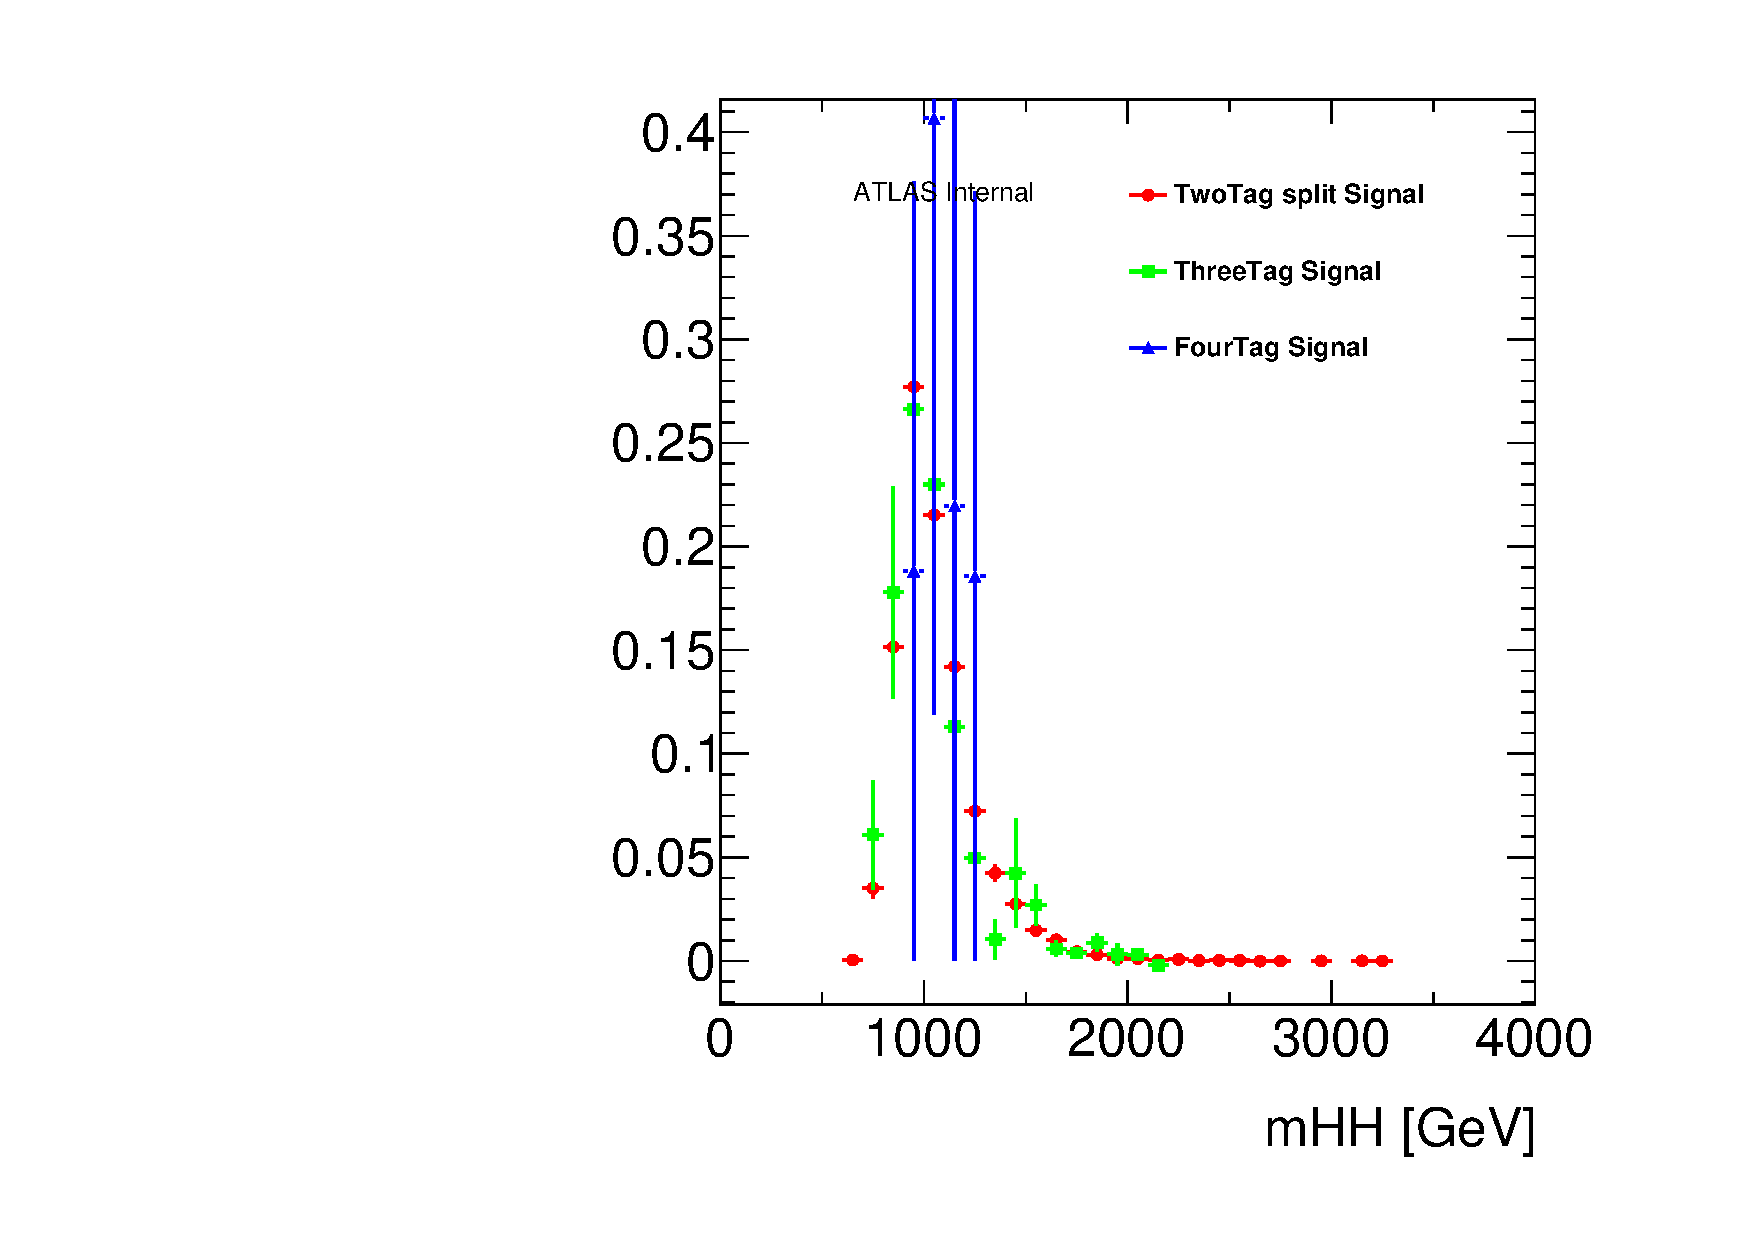
\includegraphics[width=0.45\textwidth,angle=-90]{figures/boosted/Other/ttbar_compare_mHH_l.pdf}
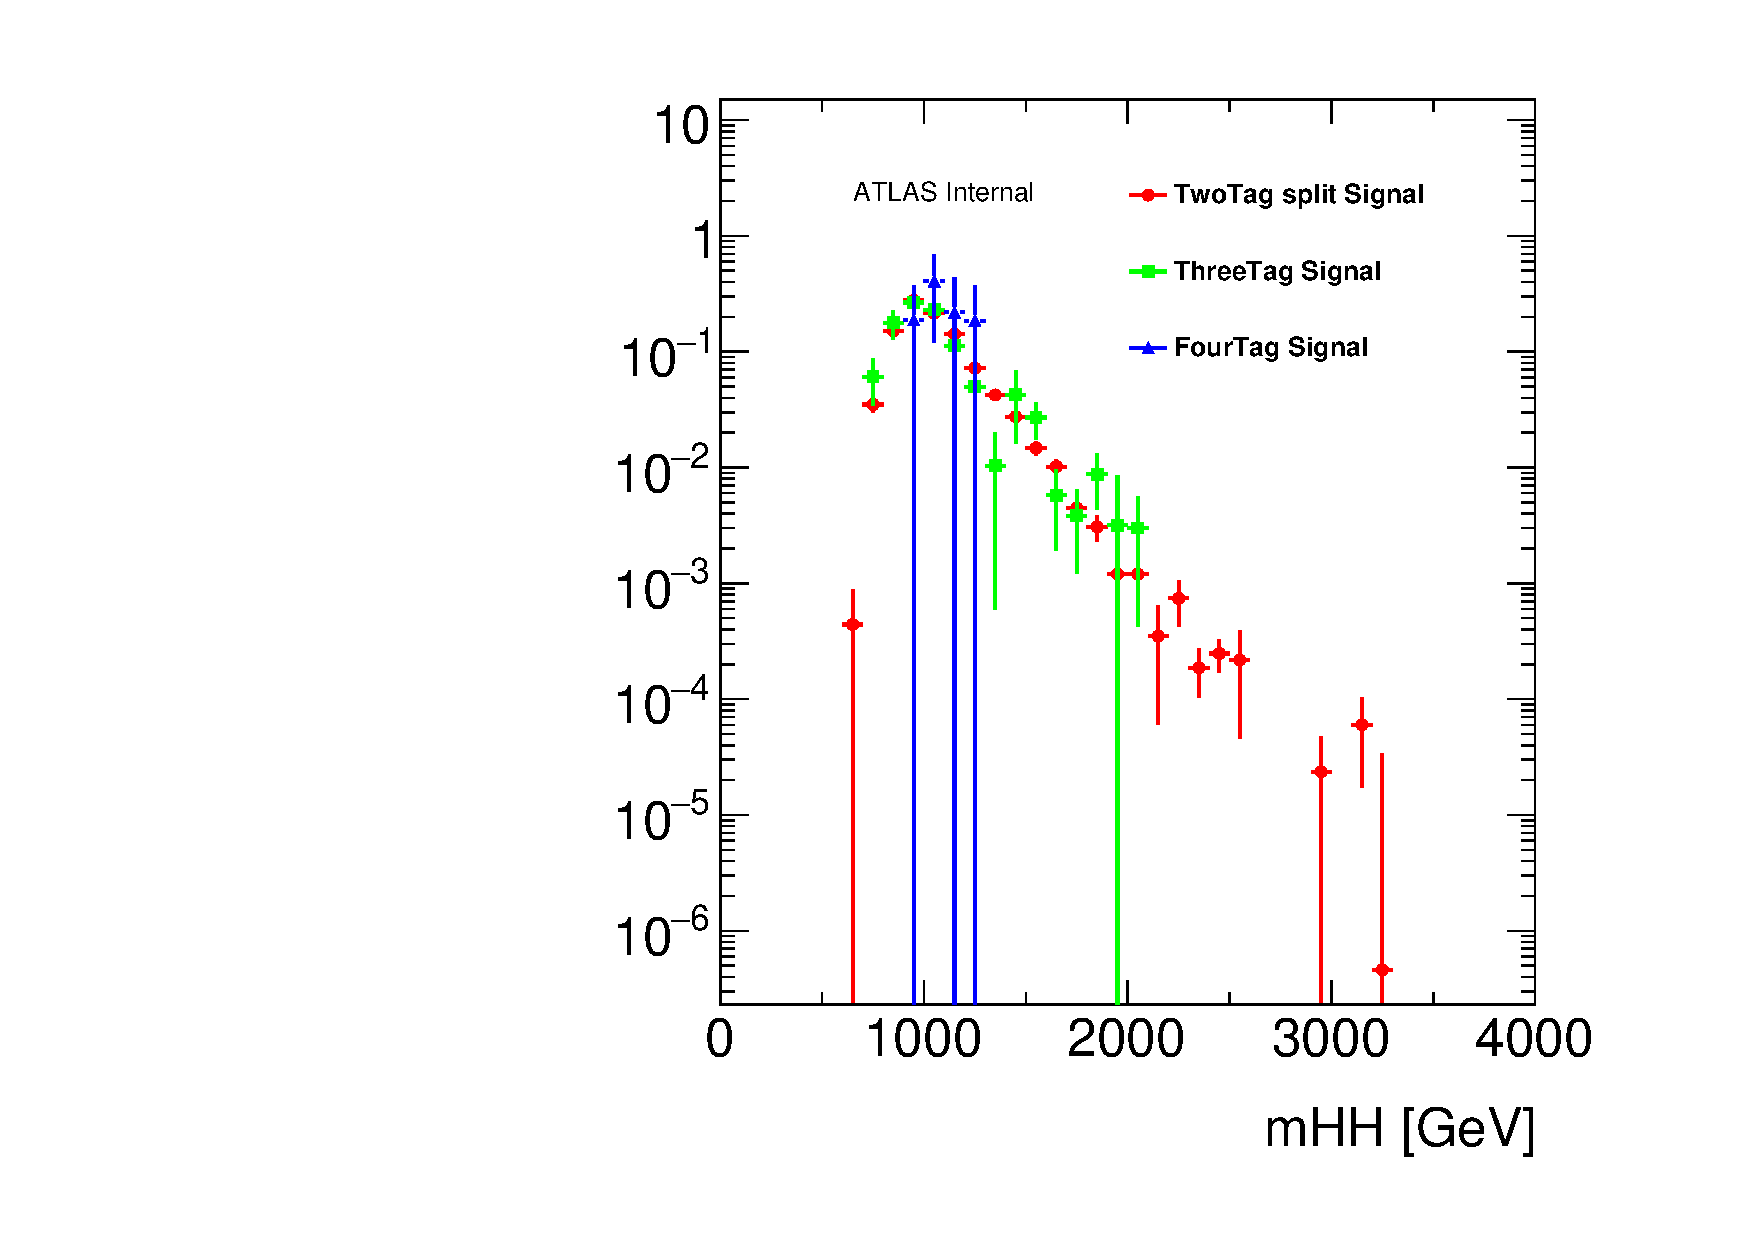
\includegraphics[width=0.45\textwidth,angle=-90]{figures/boosted/Other/ttbar_compare_mHH_l_1.pdf}
\caption{Comparison of the 4$b$, 3$b$ and 2$b$s signal region $t\bar{t}$ dijet mass shape. On the left is the linear scale, and on the right is the log scale. Both distributions are normalized to 1 for comparison.}
\label{fig:signal-region-ttbar-compare}
\end{center}
\end{figure}

%The choice of smoothing upper bound of \textbf{XXX} TeV was chosen so as not to be sensitive to possible signals in the very high mass $0b$ SR where the background estimation is performed, but where the background is likely very low.  We also want to ensure that signals as large as those at the boundary of our expected signal strength limits would not have a significant impact on our background predictions from the $2b$ SR.  Therefore, using the rough expected signal strength limits found in  Appendix~\ref{sec:boosted-optimization},  we scale the signal predictions by this signal strength limit.  We determine the maximum mass which is used in the smoothing function fit by first fitting up to a defined  point, and extrapolating the background prediction to higher mass.  We compare the extrapolation with the signal-strength-limit scaled signal prediction in a $\pm200$ GeV window around a signal mass peak.  If the signal contamination is small compared the the background prediction (at the few percent level), we consider this region safe and extend the fit maximum to higher mass. We determine the maximum fitting point by starting with a fit maximum of 1500 GeV, and comparing to an 1800 GeV signal.  The resulting S/B is <2\%, and thus is considered safe.  We then extend the fit to 1800 GeV maximum, and compare to a 2000 GeV signal.  In this case, the observed S/B is <5\%, and thus considered safe.  When extending the fit to 2000 GeV, and comparing with the 2250 GeV signal prediction, the resulting S/B was roughly 17\%.  Thus we stopped the iterative search, and fix the fit maximum to 2000 GeV.

%%\paragraph{}
Figure~\ref{fig:signal-region-4b-smoothing} shows the smoothing fits for the  QCD background and the \ttbar\ background in the $4b$ signal region.  Figure~\ref{fig:signal-region-3b-smoothing} shows the same for the $3b$ signal region. Figure~\ref{fig:signal-region-2bs-smoothing} shows the same for the $2bs$ signal region. The smoothing statistical uncertainties are also shown on these two plots. More additional uncertainties, such as uncertainty from choice of smoothing function, will be discussed in the Section~\ref{unc-smooth-qcd-in-sr}.

%%\paragraph{}
The final smoothed background predictions for the $4b$ and $3b$ and $2bs$ signal regions can be found in Figure~\ref{fig:signal-region-smooth-bkg}. This includes smoothing statistical uncertainties only. More details on other systematics, including smoothing systematics, shape uncertainties and other sources of uncertainties would be discussed in Section~\ref{unc-smooth-qcd-in-sr}.

%%\paragraph{}
Uncertainties on the fit parameters are propagated as systematic uncertainties, though they are essentially replacing the bin-by-bin statistical uncertainties of the background estimates (which are not used once smoothing is applied). Correlations in the fit parameters of the backgrounds are taken into account when propagating the uncertainties, as described in Appendix~\ref{app:correrr}.

% %%\paragraph{}
% Note that while the functional form is only fit within a restricted range for both the \ttbar\ and QCD prediction, the function was used to smooth over the entire range of $M_{JJ}>1100$ GeV for the QCD (\ttbar) prediction.

%The final smoothed signal region predictions, including all statistical and systematic uncertainties, are shown in Figure~\ref{fig:signal-region-smooth-bkg-allSYS}.


\begin{table}[htbp!]
\begin{center}
\begin{footnotesize} 
\begin{tabular}{c|c|c|c|c|c|c} 
Region & $ a_{t\bar{t}}$ & $ b_{t\bar{t}}$ & $ c_{t\bar{t}}$ & $ a_{qcd}$ & $ b_{qcd}$ & $c_{qcd}$ \\ 
\hline\hline 
& & & & & &\\ 
FourTag & -1.02 $\pm$ 1.22 & 35.62 $\pm$ 10.83 & 9.05 $\pm$ 9.59 & 7.75 $\pm$ 1.8 & -18.0 $\pm$ 16.75 & 54.36 $\pm$ 14.28\\ 
ThreeTag & 2.83 $\pm$ 1.22 & 35.62 $\pm$ 10.83 & 9.05 $\pm$ 9.59 & 10.42 $\pm$ 1.73 & -27.1 $\pm$ 15.78 & 56.91 $\pm$ 13.89\\ 
TwoTag split & 5.21 $\pm$ 1.22 & 35.62 $\pm$ 10.83 & 9.05 $\pm$ 9.59 & 7.74 $\pm$ 0.36 & 7.22 $\pm$ 3.11 & 24.54 $\pm$ 2.78\\ 
& & & & & &\\ 
\hline\hline 
\end{tabular} 
\end{footnotesize} 
\newline 

\caption{Smoothing parameters in $4b$ and $3b$ and $2bs$ signal regions, the correlation between parameters is almost always 0.99.}
\label{tab:smoothparams_l}
\end{center}
\end{table}


\begin{figure}[htbp!]
\begin{center}
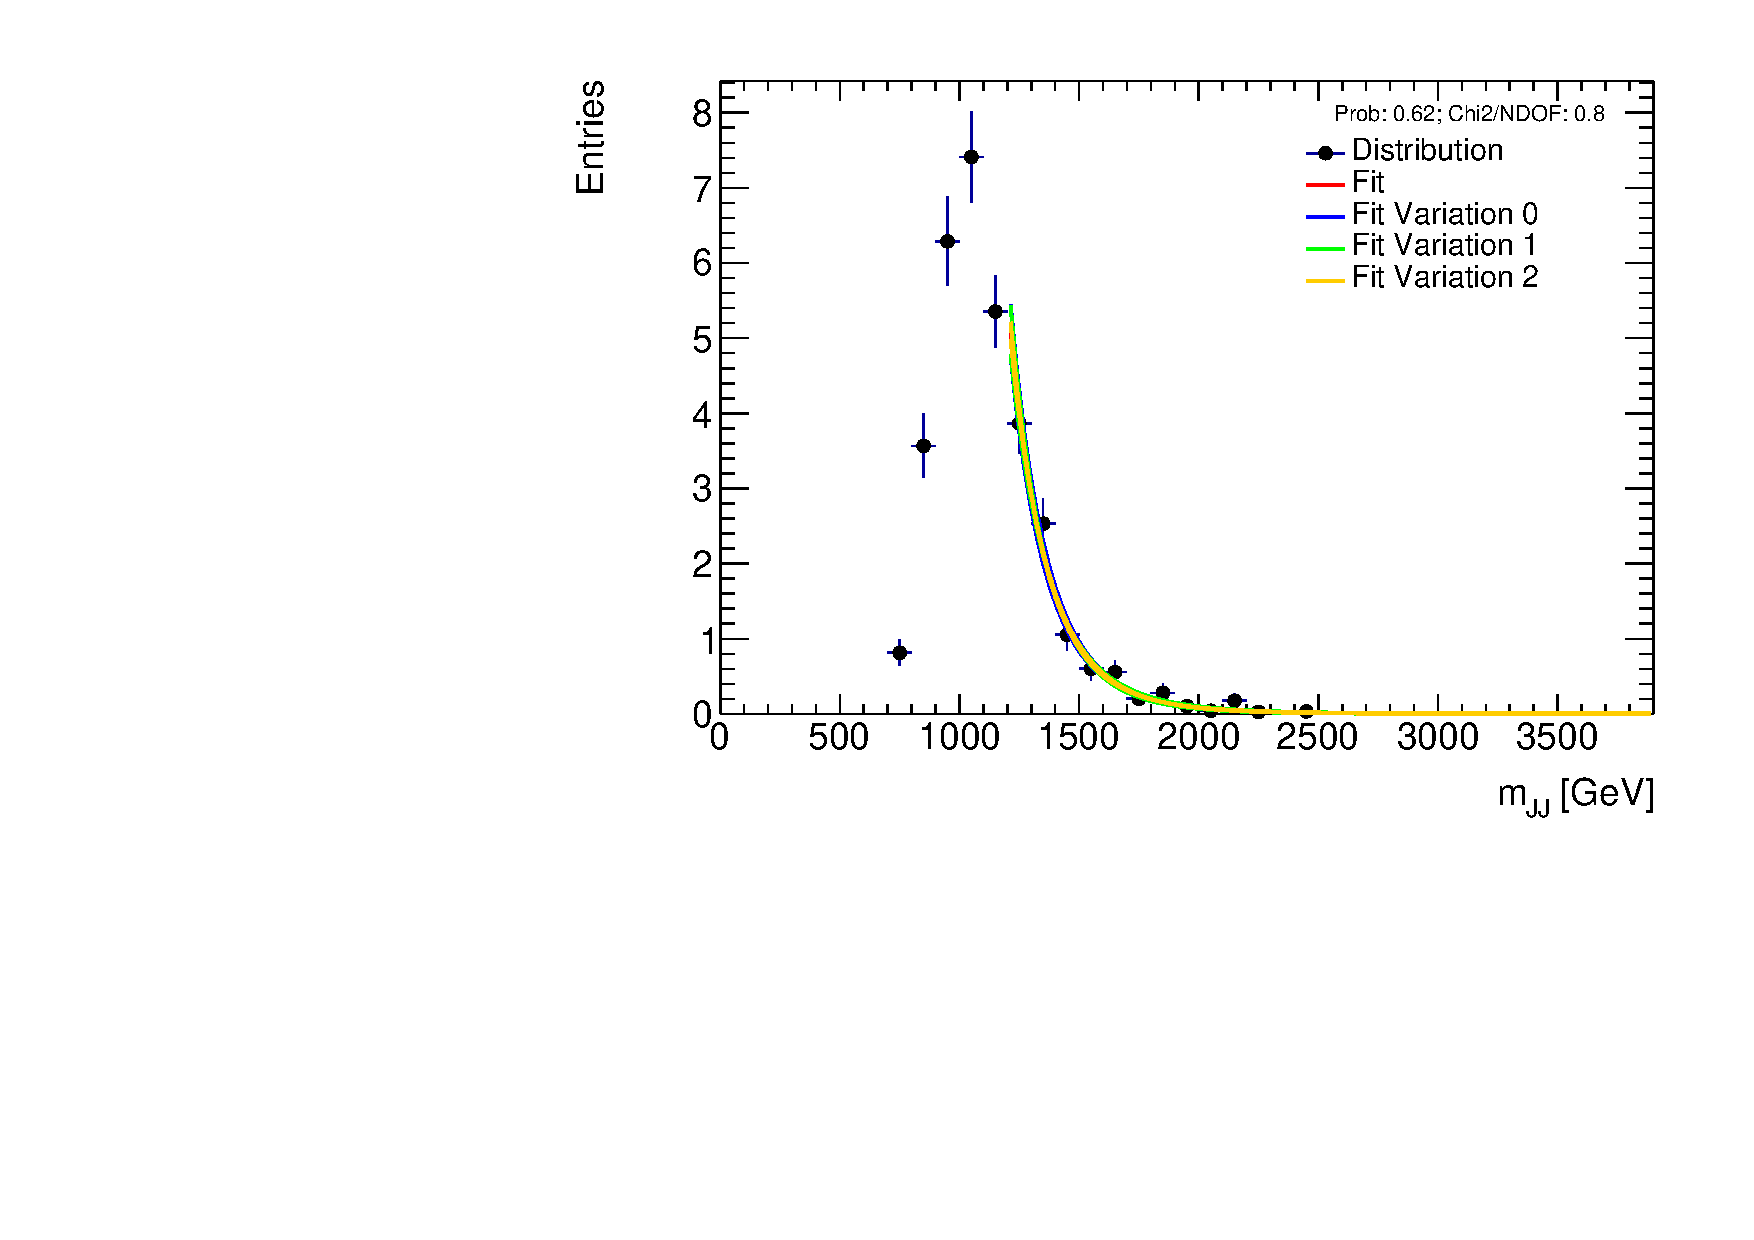
\includegraphics[width=0.45\textwidth,angle=-90]{figures/boosted/Smooth/qcd_est_FourTag_Signal_mHH_l.pdf}
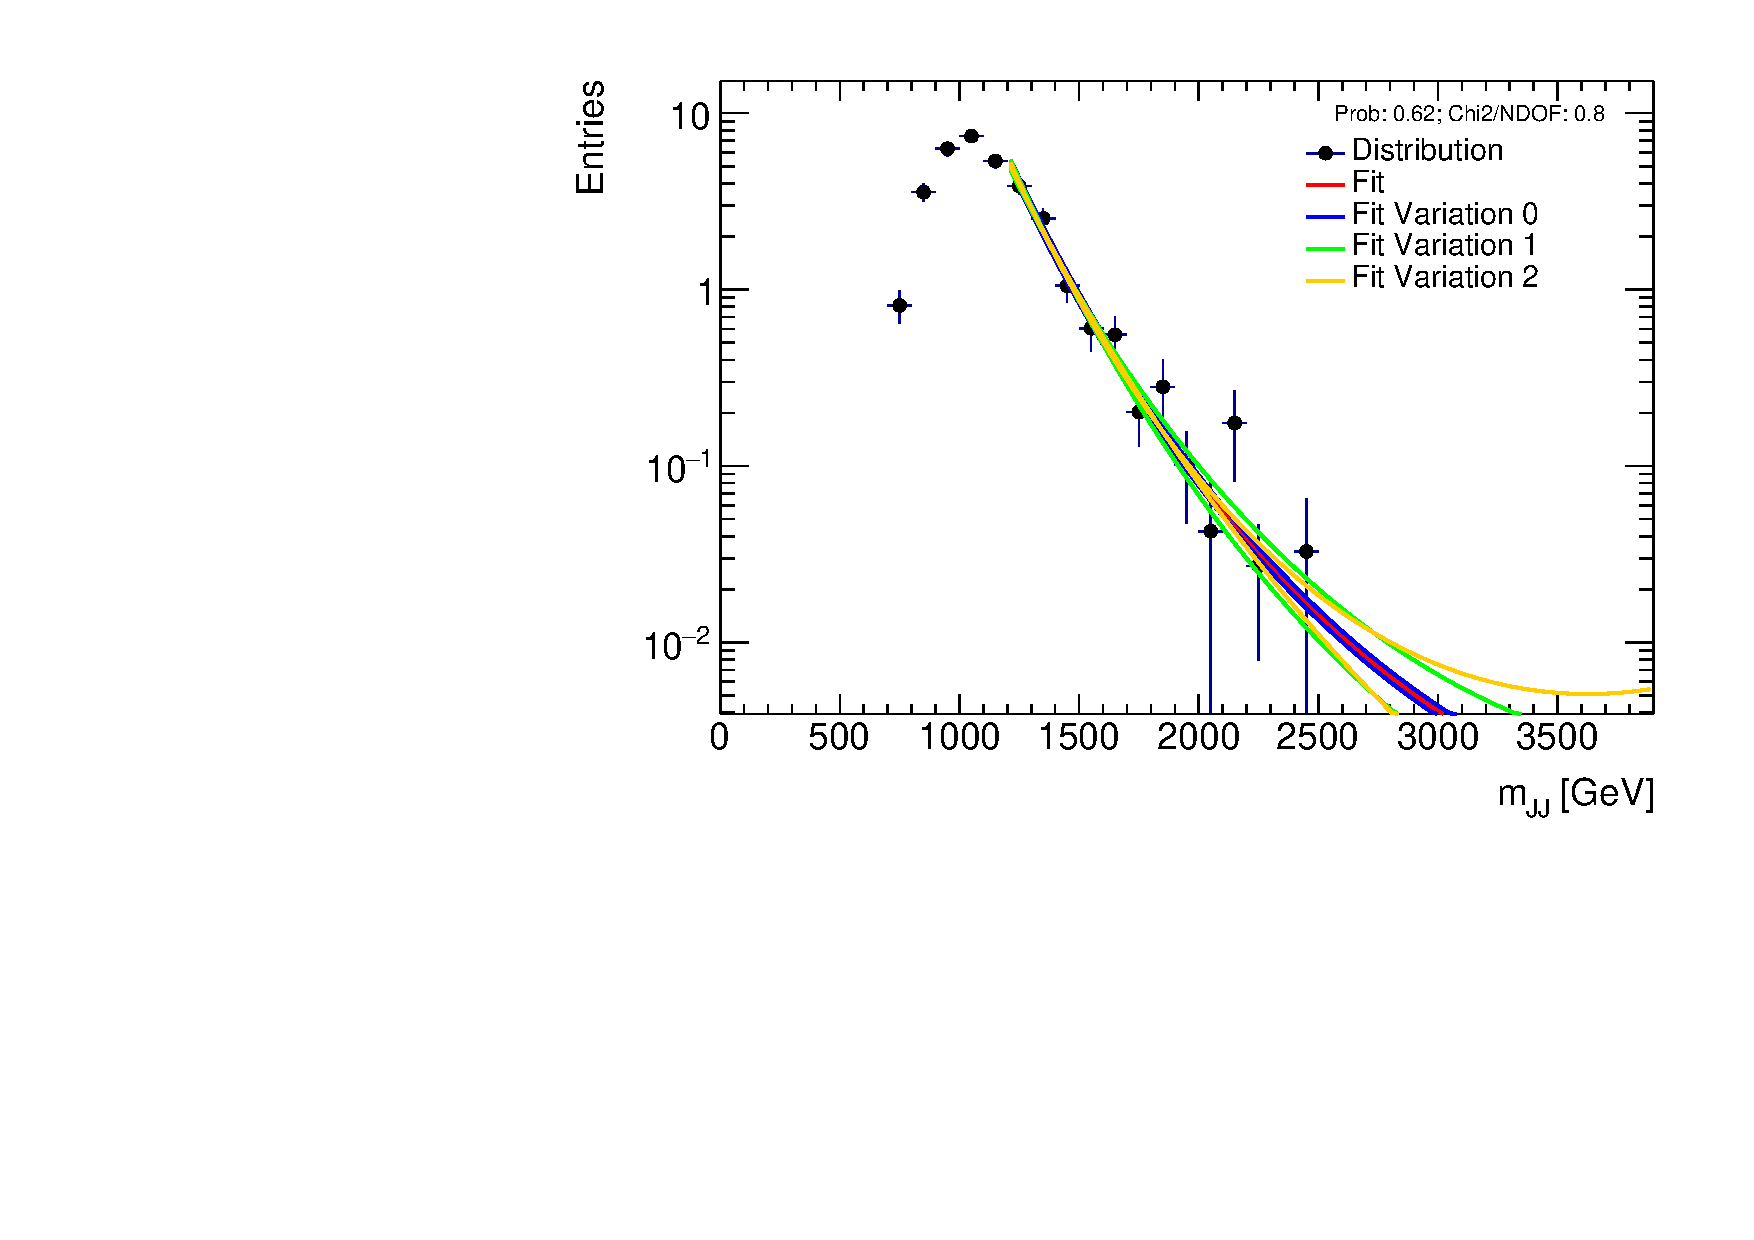
\includegraphics[width=0.45\textwidth,angle=-90]{figures/boosted/Smooth/qcd_est_FourTag_Signal_mHH_l_l.pdf}\\ 
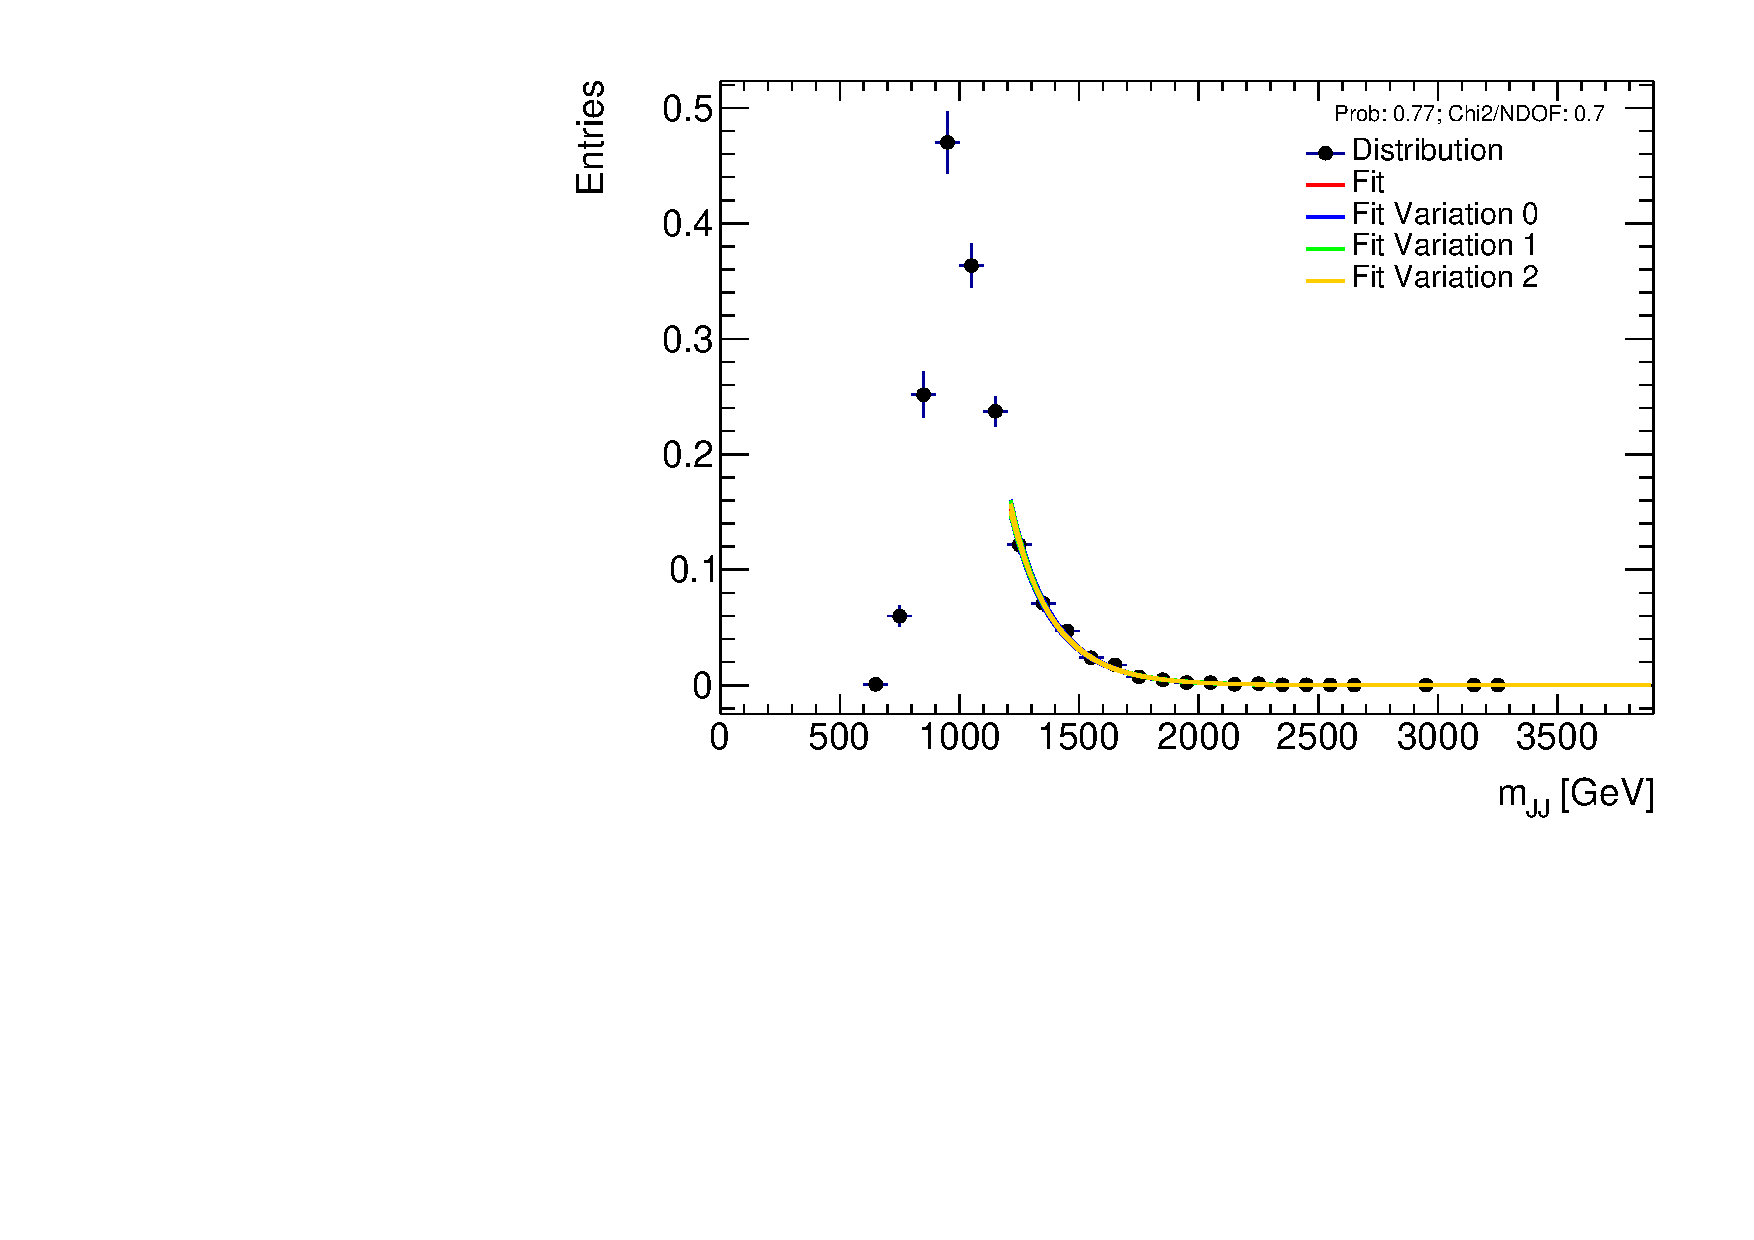
\includegraphics[width=0.45\textwidth,angle=-90]{figures/boosted/Smooth/ttbar_est_FourTag_Signal_mHH_l.pdf}
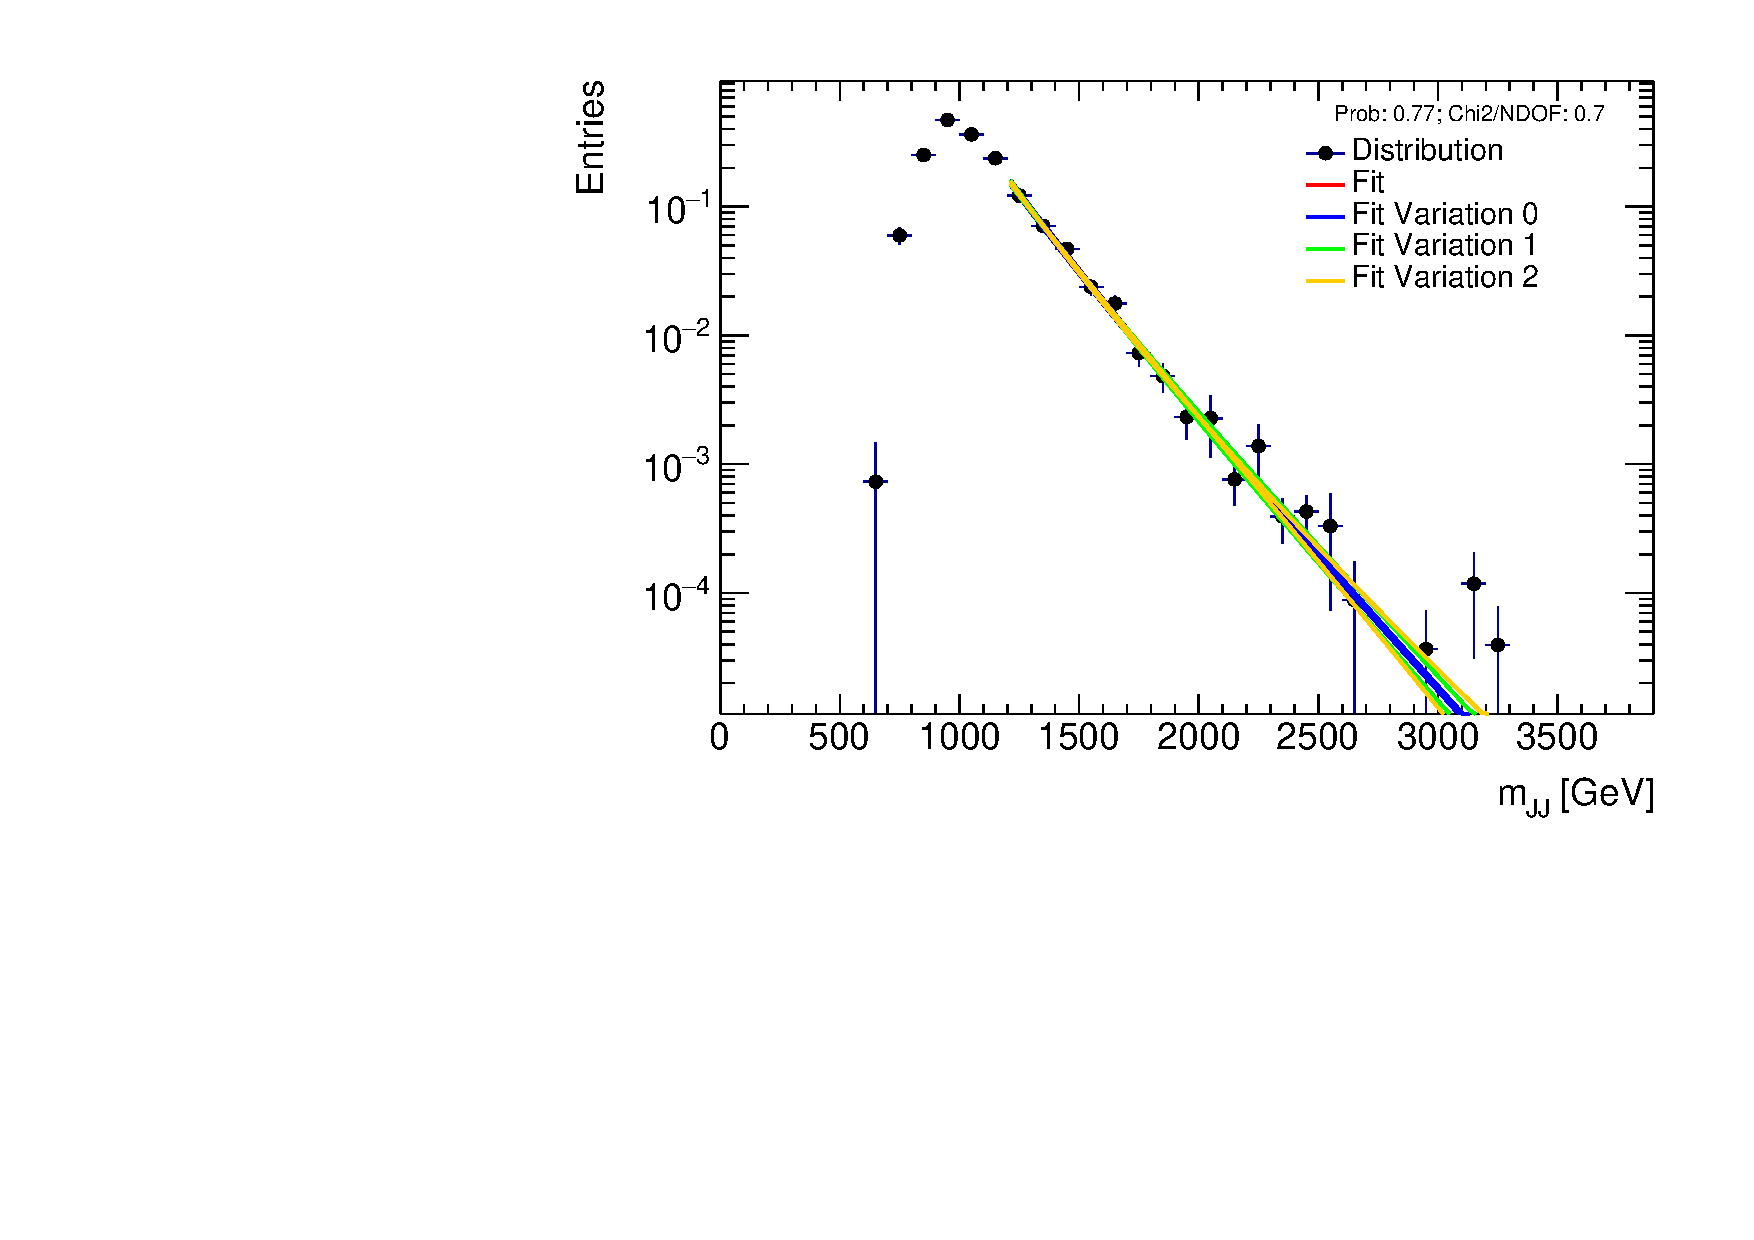
\includegraphics[width=0.45\textwidth,angle=-90]{figures/boosted/Smooth/ttbar_est_FourTag_Signal_mHH_l_l.pdf}\\
\caption{Fits for background smoothing are shown for QCD (top row) and $t\bar{t}$ (bottom row) in the $4b$ signal region.  The left figures show the distributions with linear $y$-axis scale along with the fit central value and variations. The right figures show the  distributions with log $y$-axis scale along with the fit central value and the fit variations as determined by the varying the fit parameters within uncertainties whilst taking into account parameter correlations. }
\label{fig:signal-region-4b-smoothing}
\end{center}
\end{figure}

\begin{figure}[htbp!]
\begin{center}
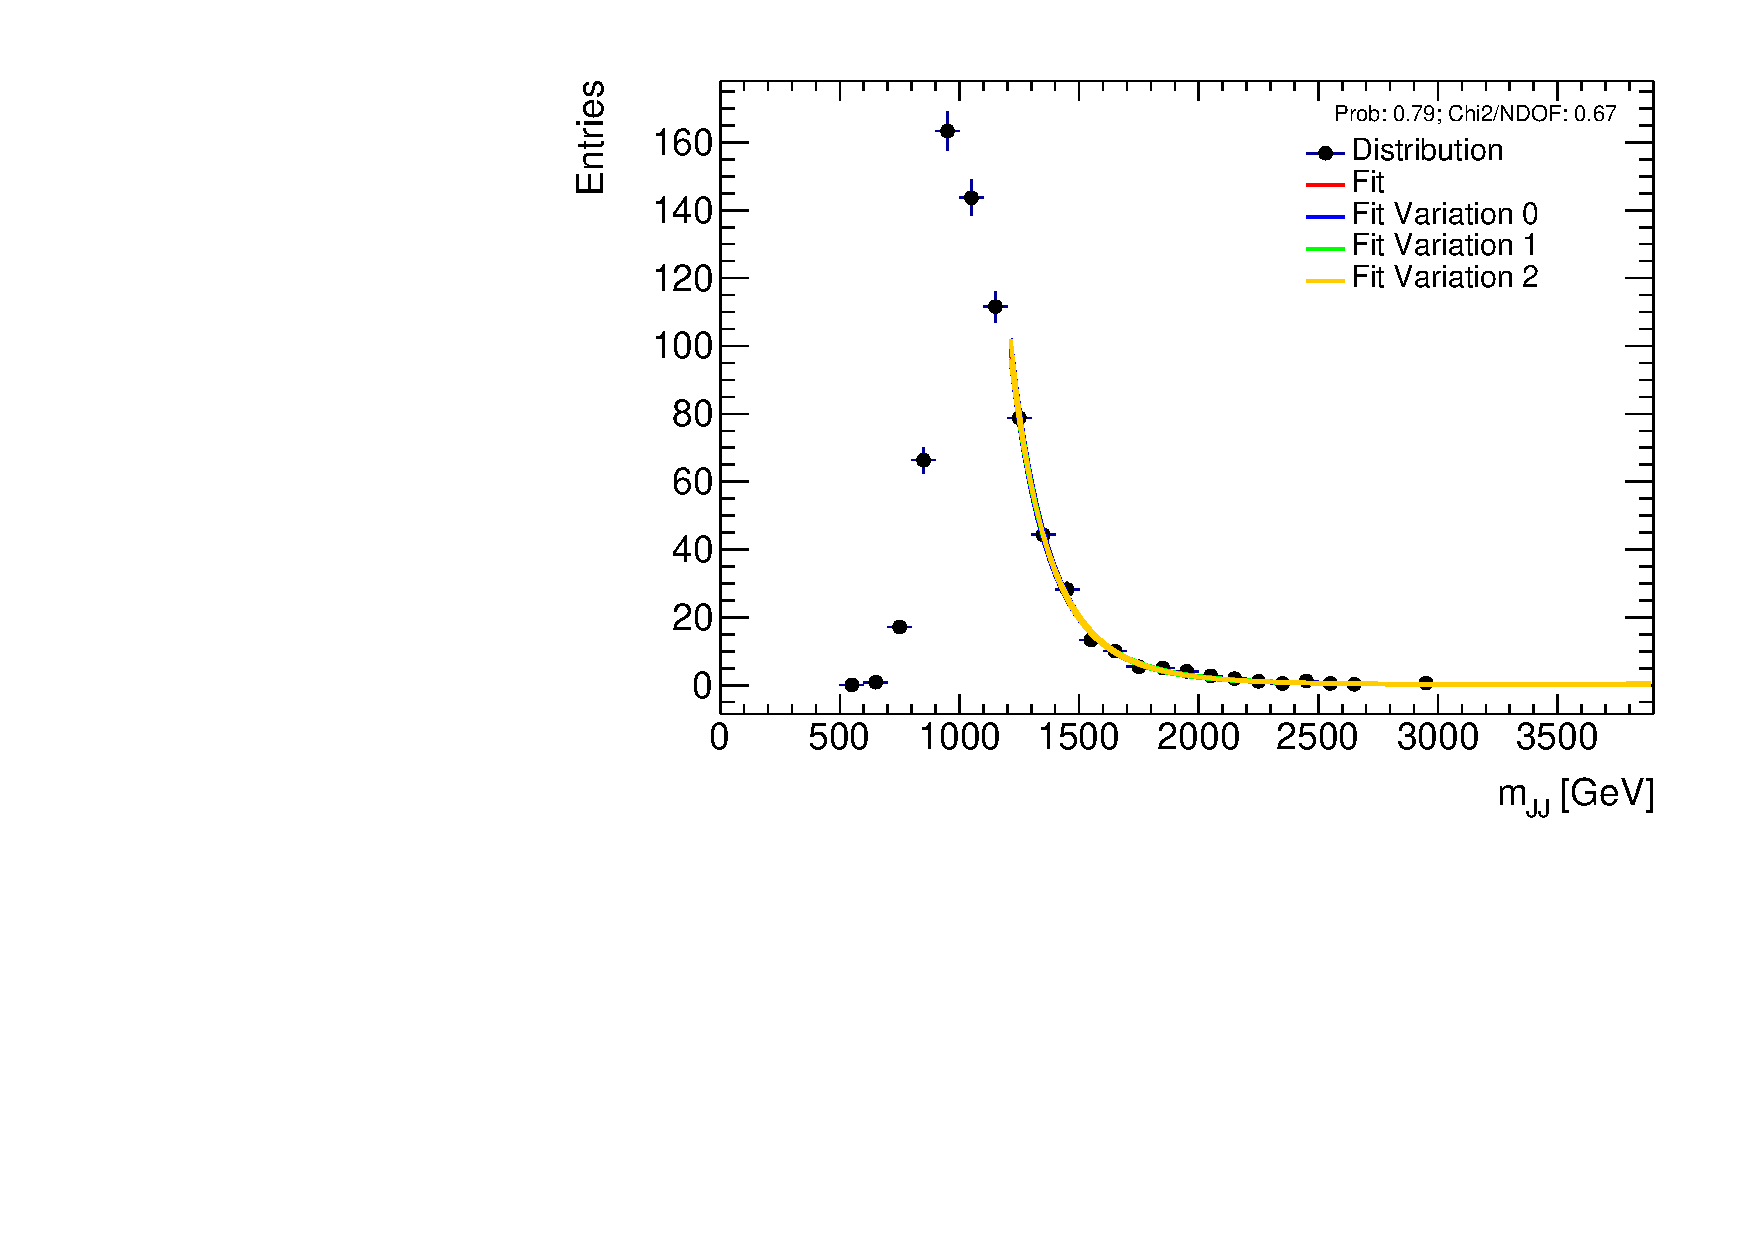
\includegraphics[width=0.45\textwidth,angle=-90]{figures/boosted/Smooth/qcd_est_ThreeTag_Signal_mHH_l.pdf}
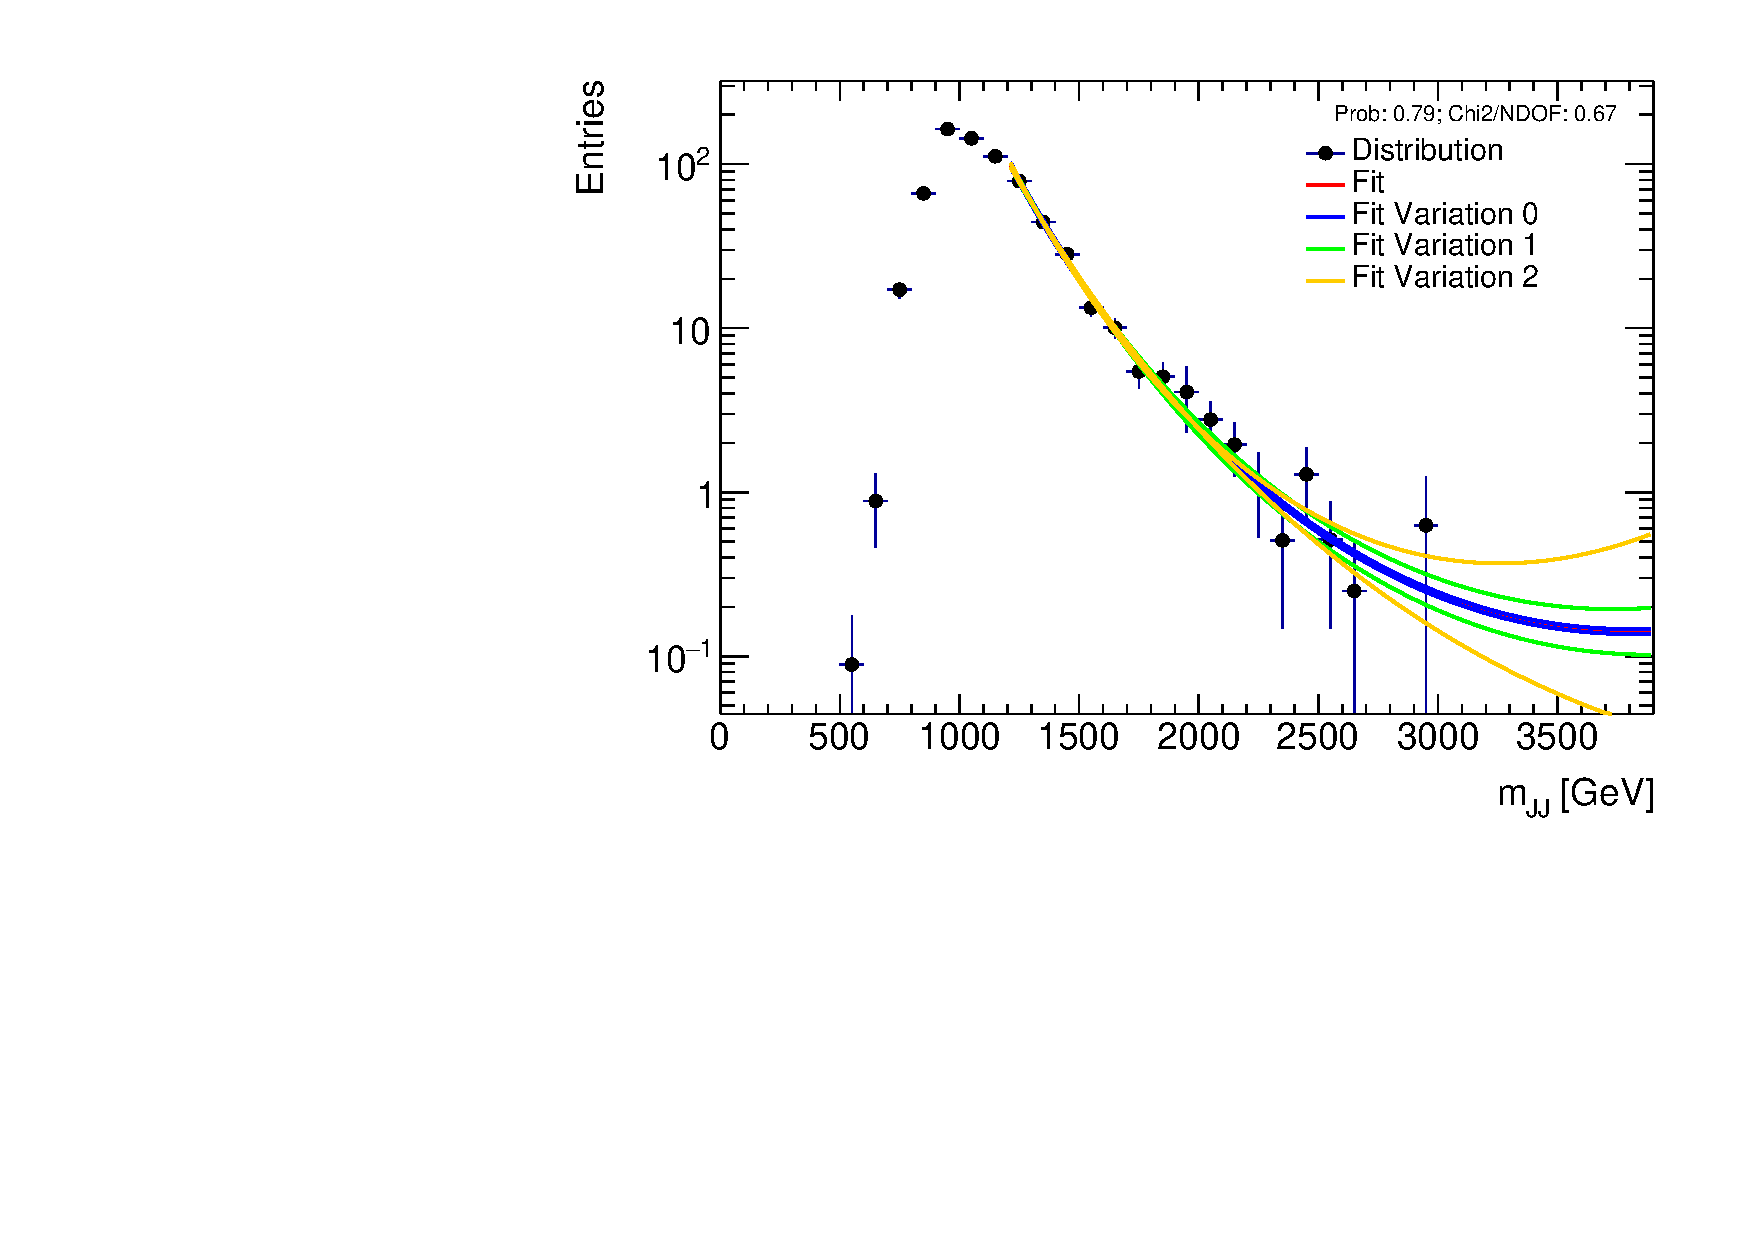
\includegraphics[width=0.45\textwidth,angle=-90]{figures/boosted/Smooth/qcd_est_ThreeTag_Signal_mHH_l_l.pdf}\\  
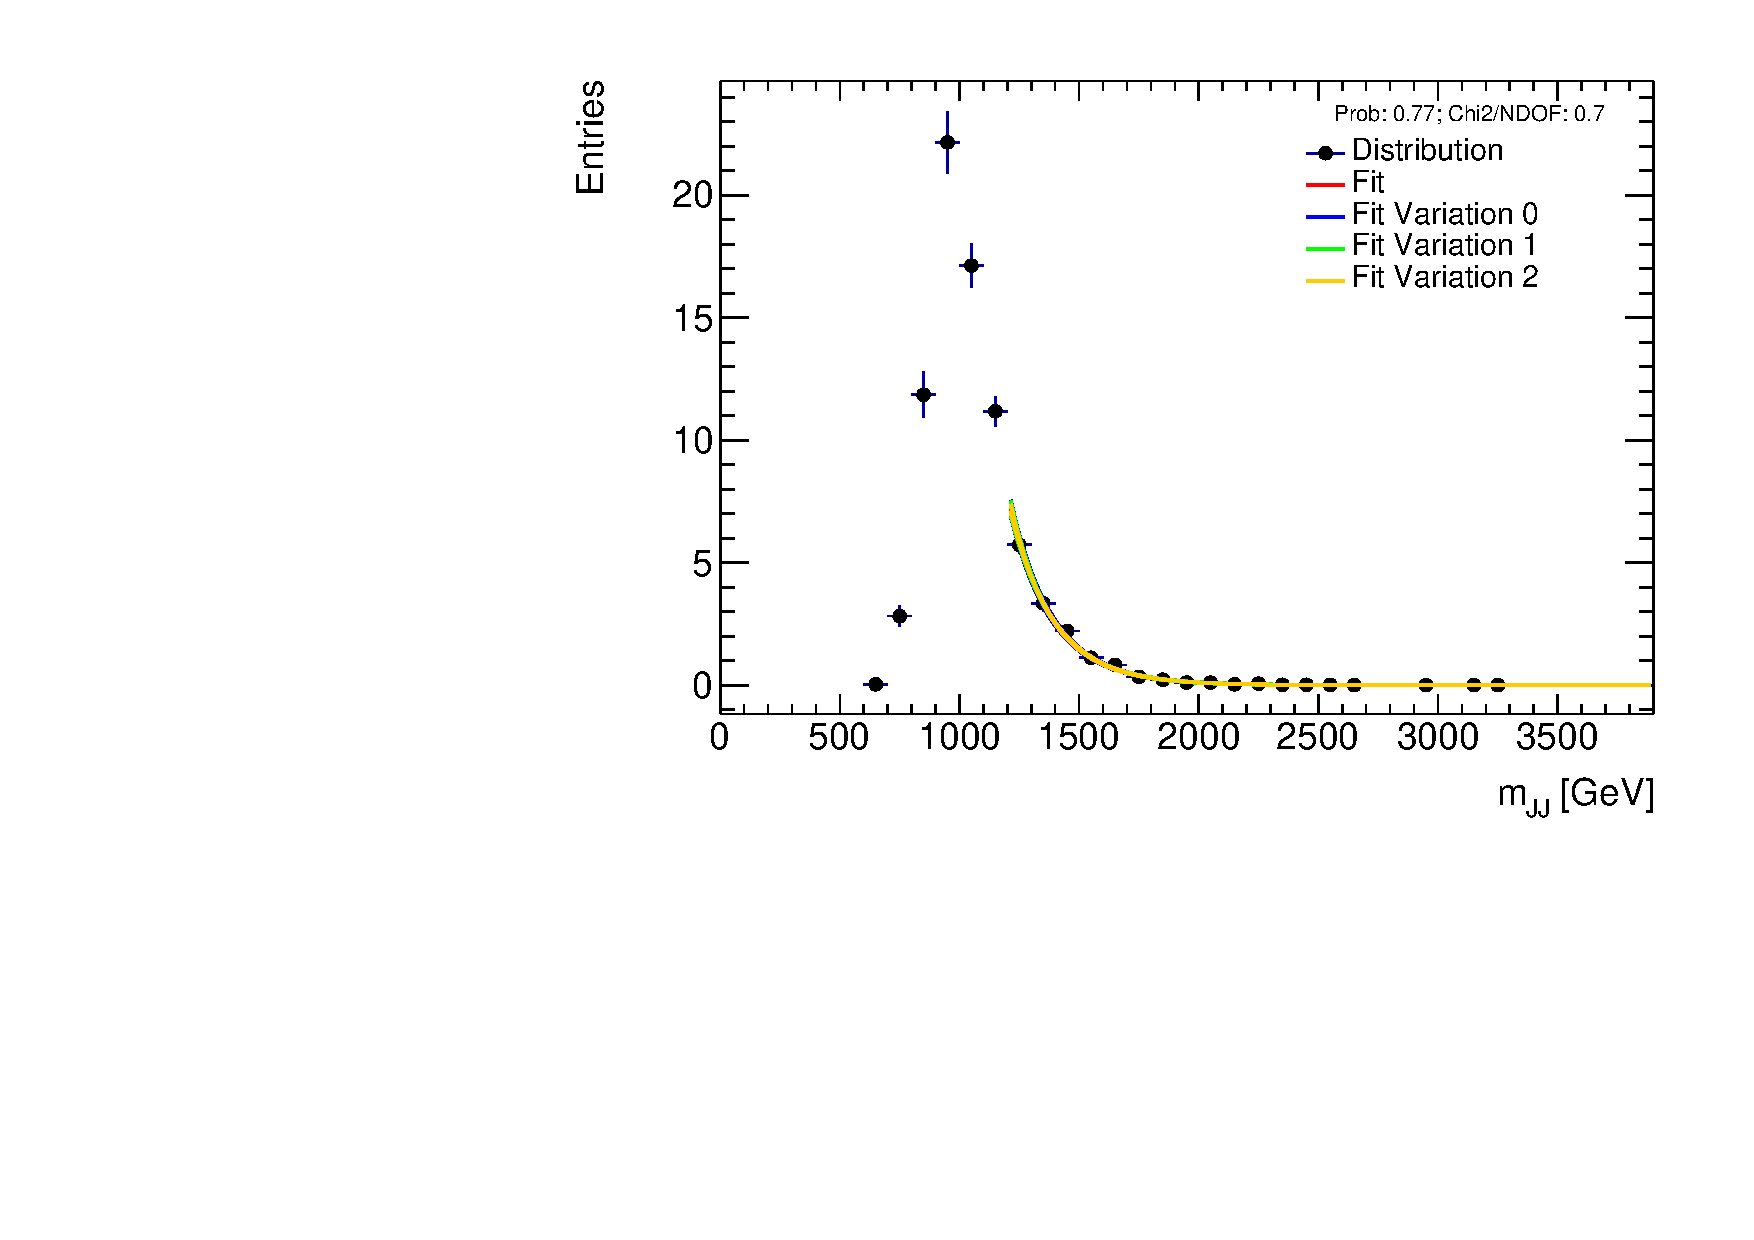
\includegraphics[width=0.45\textwidth,angle=-90]{figures/boosted/Smooth/ttbar_est_ThreeTag_Signal_mHH_l.pdf}
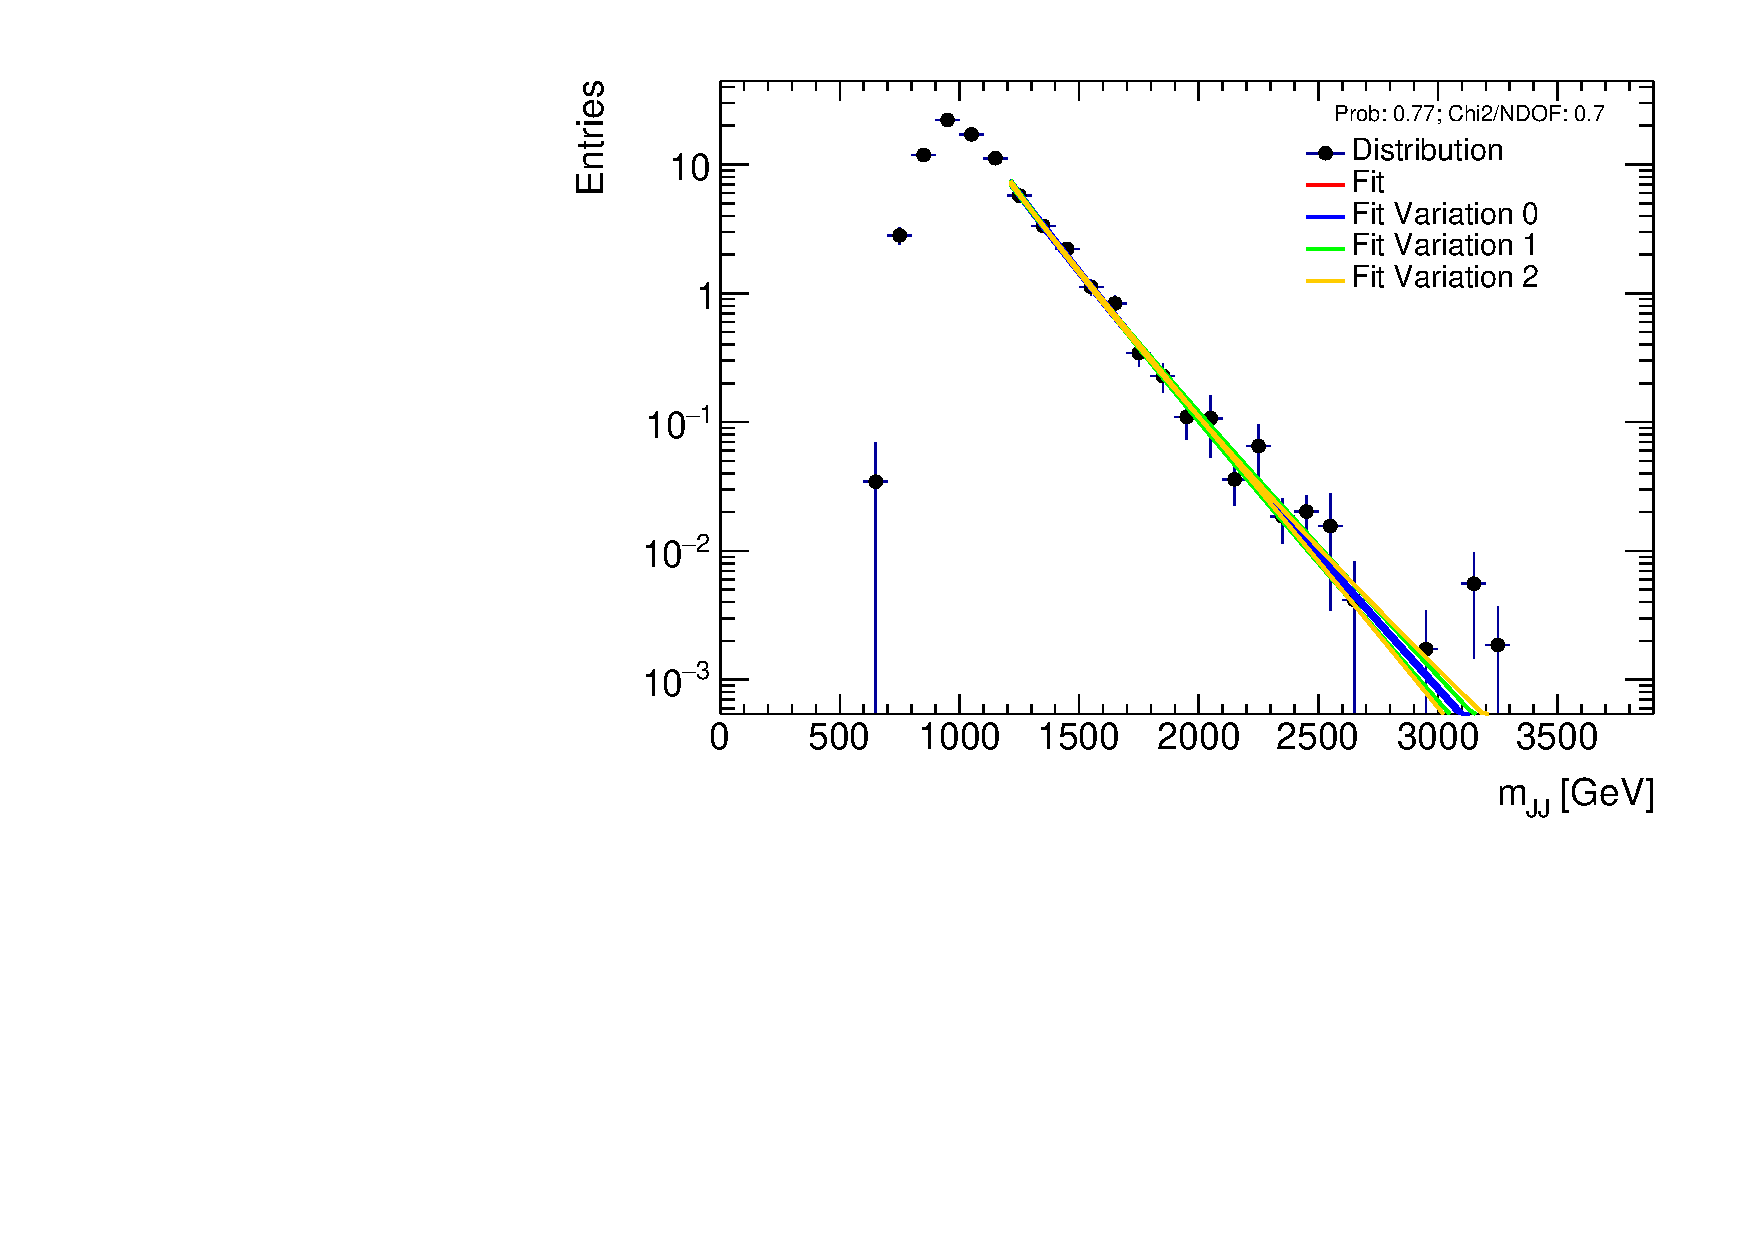
\includegraphics[width=0.45\textwidth,angle=-90]{figures/boosted/Smooth/ttbar_est_ThreeTag_Signal_mHH_l_l.pdf}\\
\caption{Fits for background smoothing are shown for QCD (top row) and $t\bar{t}$ (bottom row) in the $3b$ signal region.  The left figures show the distributions with linear $y$-axis scale along with the fit central value and variations. The right figures show the  distributions with log $y$-axis scale along with the fit central value and the fit variations as determined by the varying the fit parameters within uncertainties whilst taking into account parameter correlations. }
\label{fig:signal-region-3b-smoothing}
\end{center}
\end{figure}

\begin{figure}[htbp!]
\begin{center}
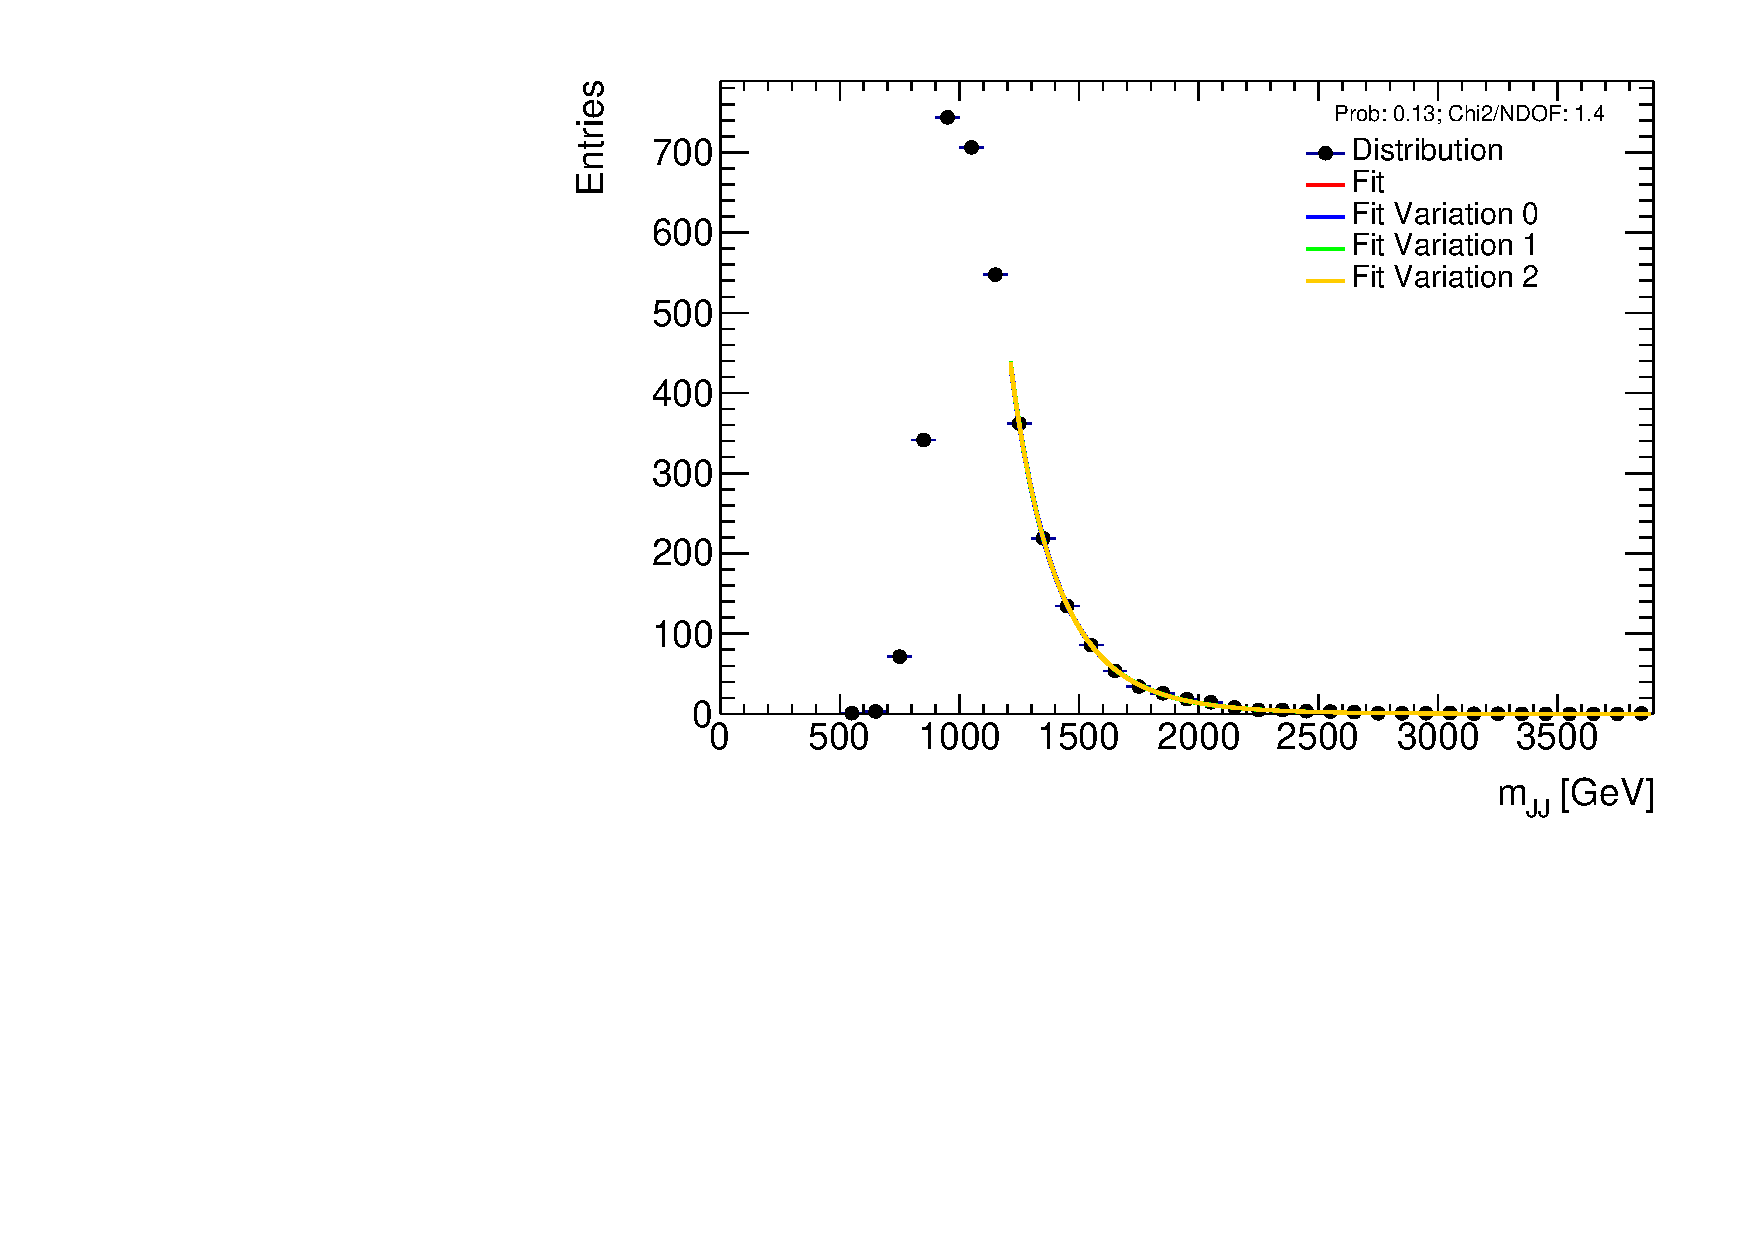
\includegraphics[width=0.45\textwidth,angle=-90]{figures/boosted/Smooth/qcd_est_TwoTag_split_Signal_mHH_l.pdf}
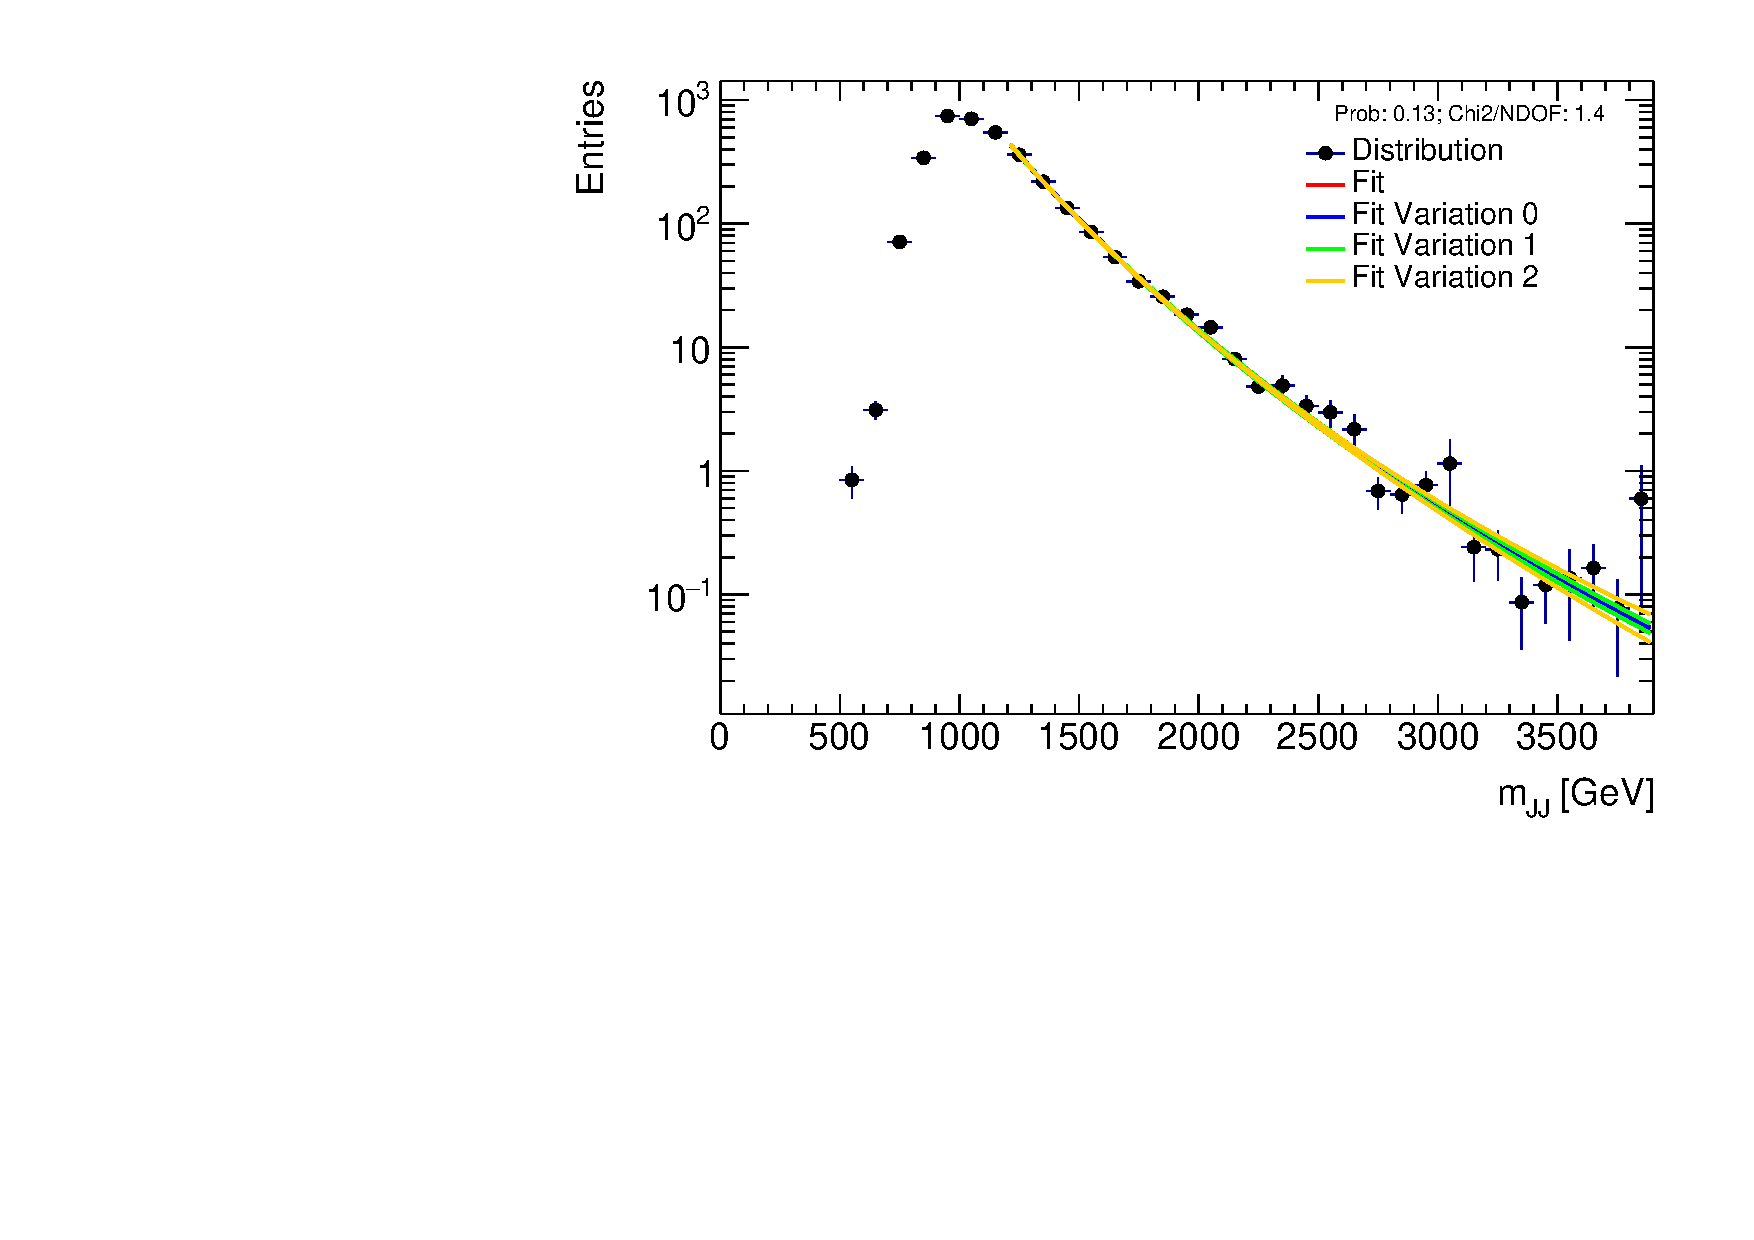
\includegraphics[width=0.45\textwidth,angle=-90]{figures/boosted/Smooth/qcd_est_TwoTag_split_Signal_mHH_l_l.pdf}\\ 
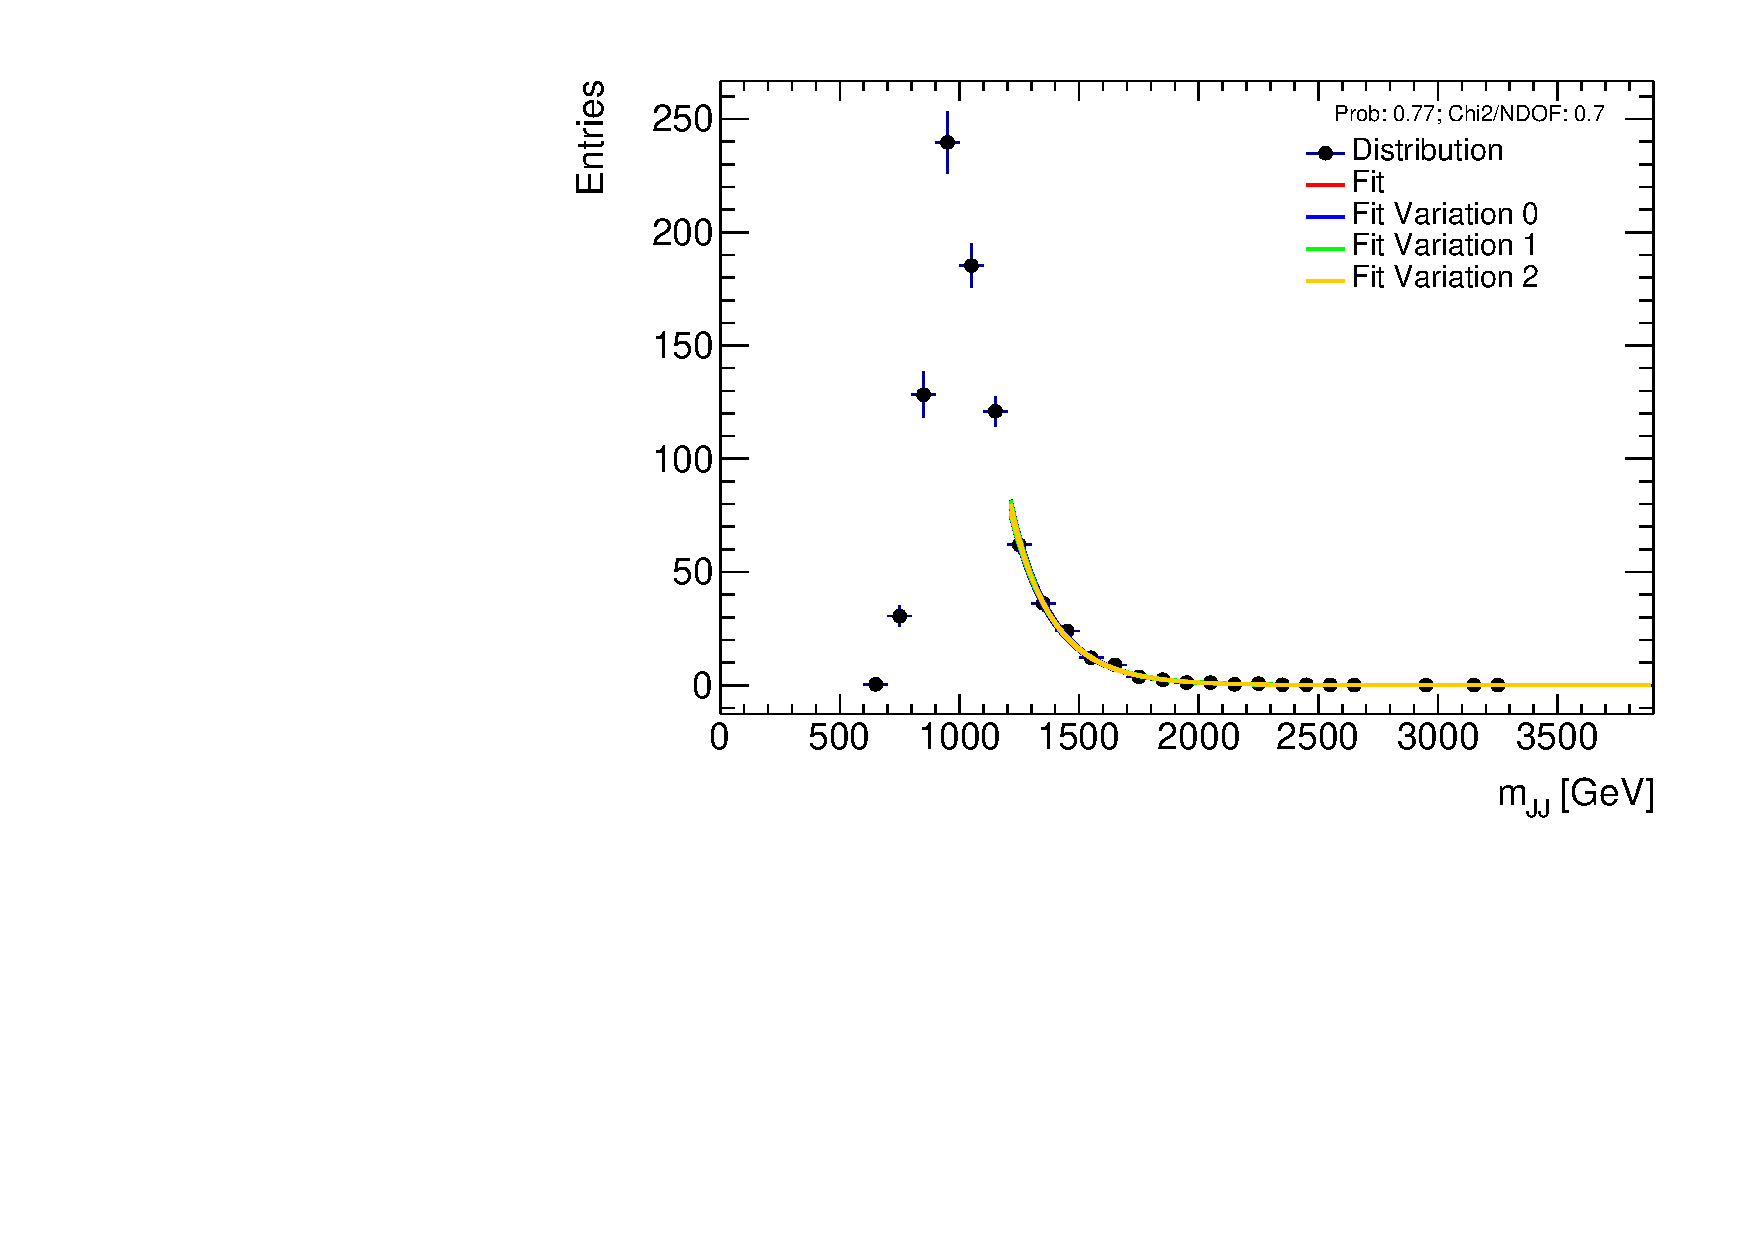
\includegraphics[width=0.45\textwidth,angle=-90]{figures/boosted/Smooth/ttbar_est_TwoTag_split_Signal_mHH_l.pdf}
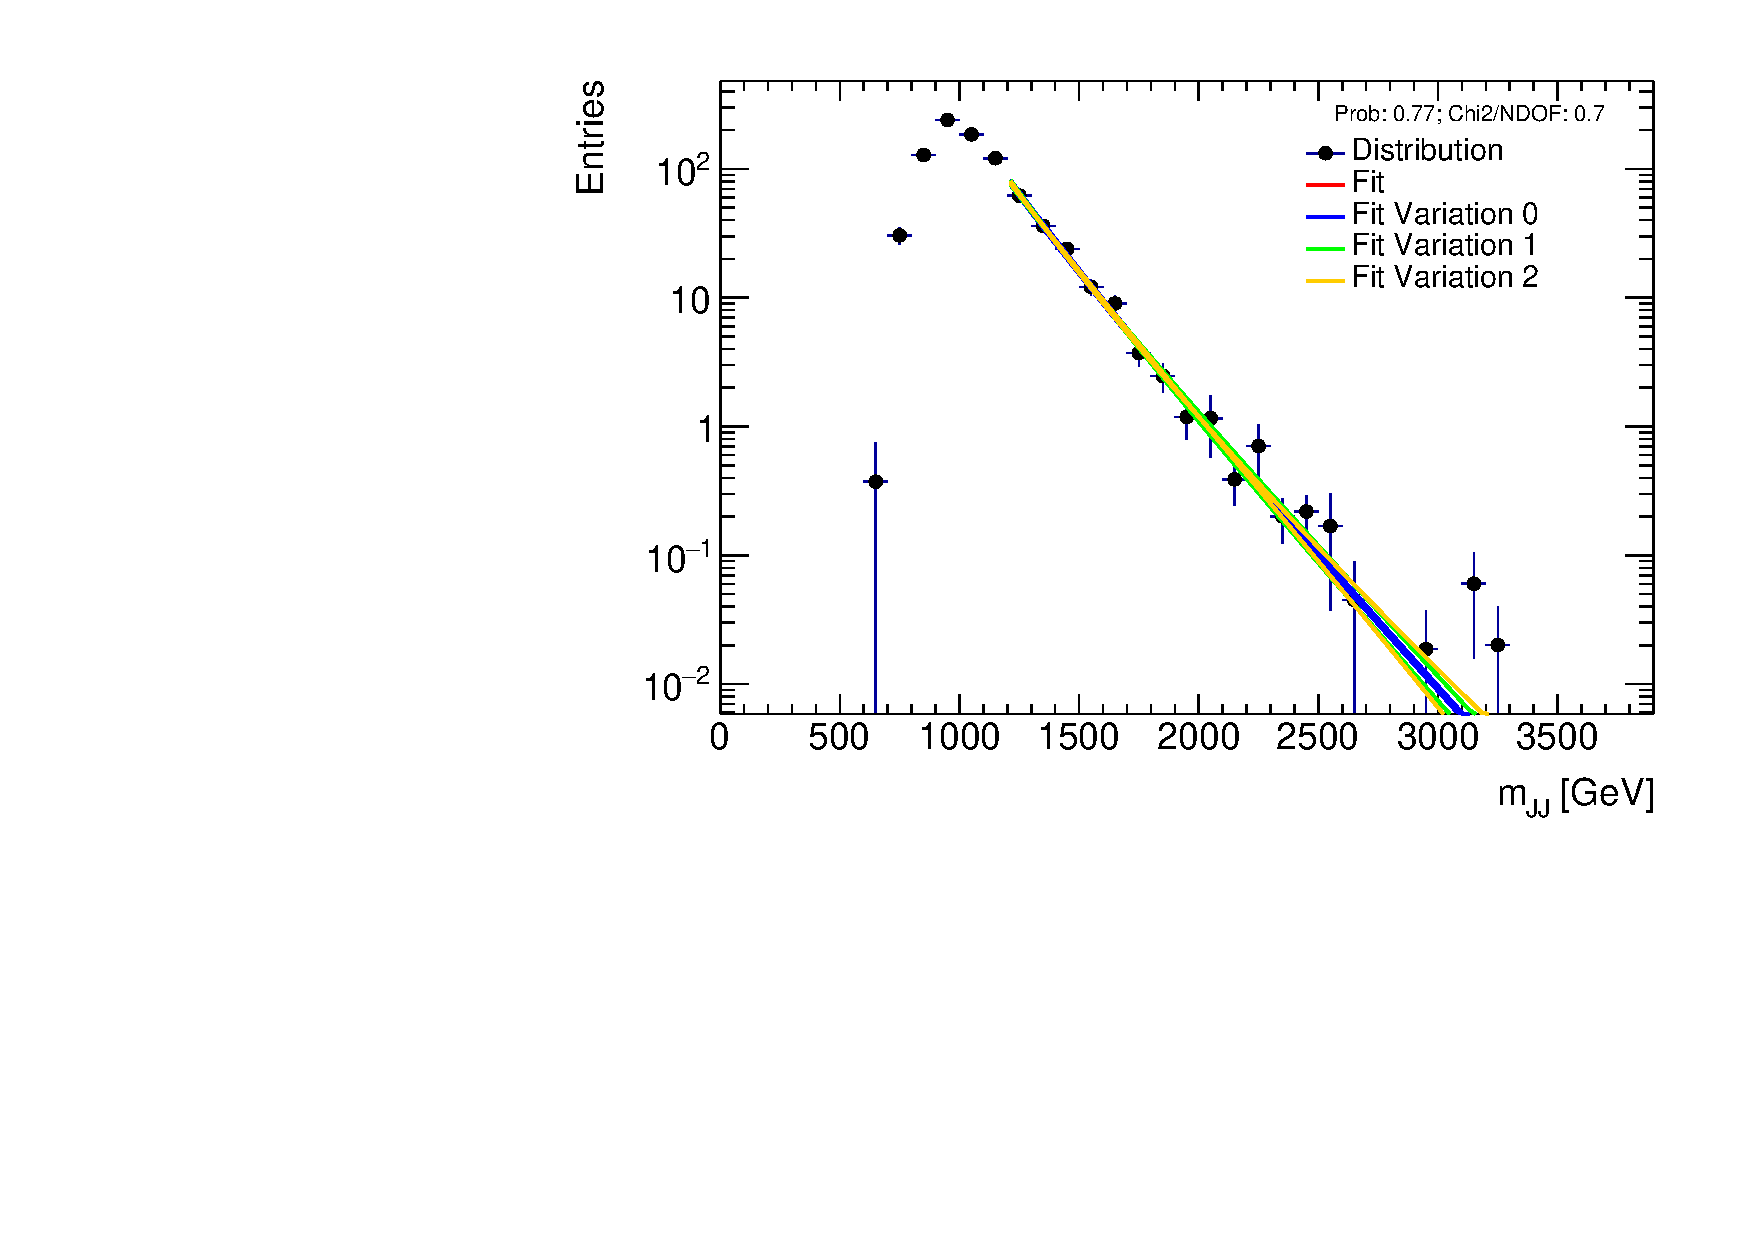
\includegraphics[width=0.45\textwidth,angle=-90]{figures/boosted/Smooth/ttbar_est_TwoTag_split_Signal_mHH_l_l.pdf}
\caption{Fits for background smoothing are shown for QCD (top row) and $t\bar{t}$ (bottom row) in the $2bs$ signal region.  The left figures show the distributions with linear $y$-axis scale along with the fit central value and variations. The right figures show the  distributions with log $y$-axis scale along with the fit central value and the fit variations as determined by the varying the fit parameters within uncertainties whilst taking into account parameter correlations. }
\label{fig:signal-region-2bs-smoothing}
\end{center}
\end{figure}


\begin{figure}[htbp!]
\begin{center}
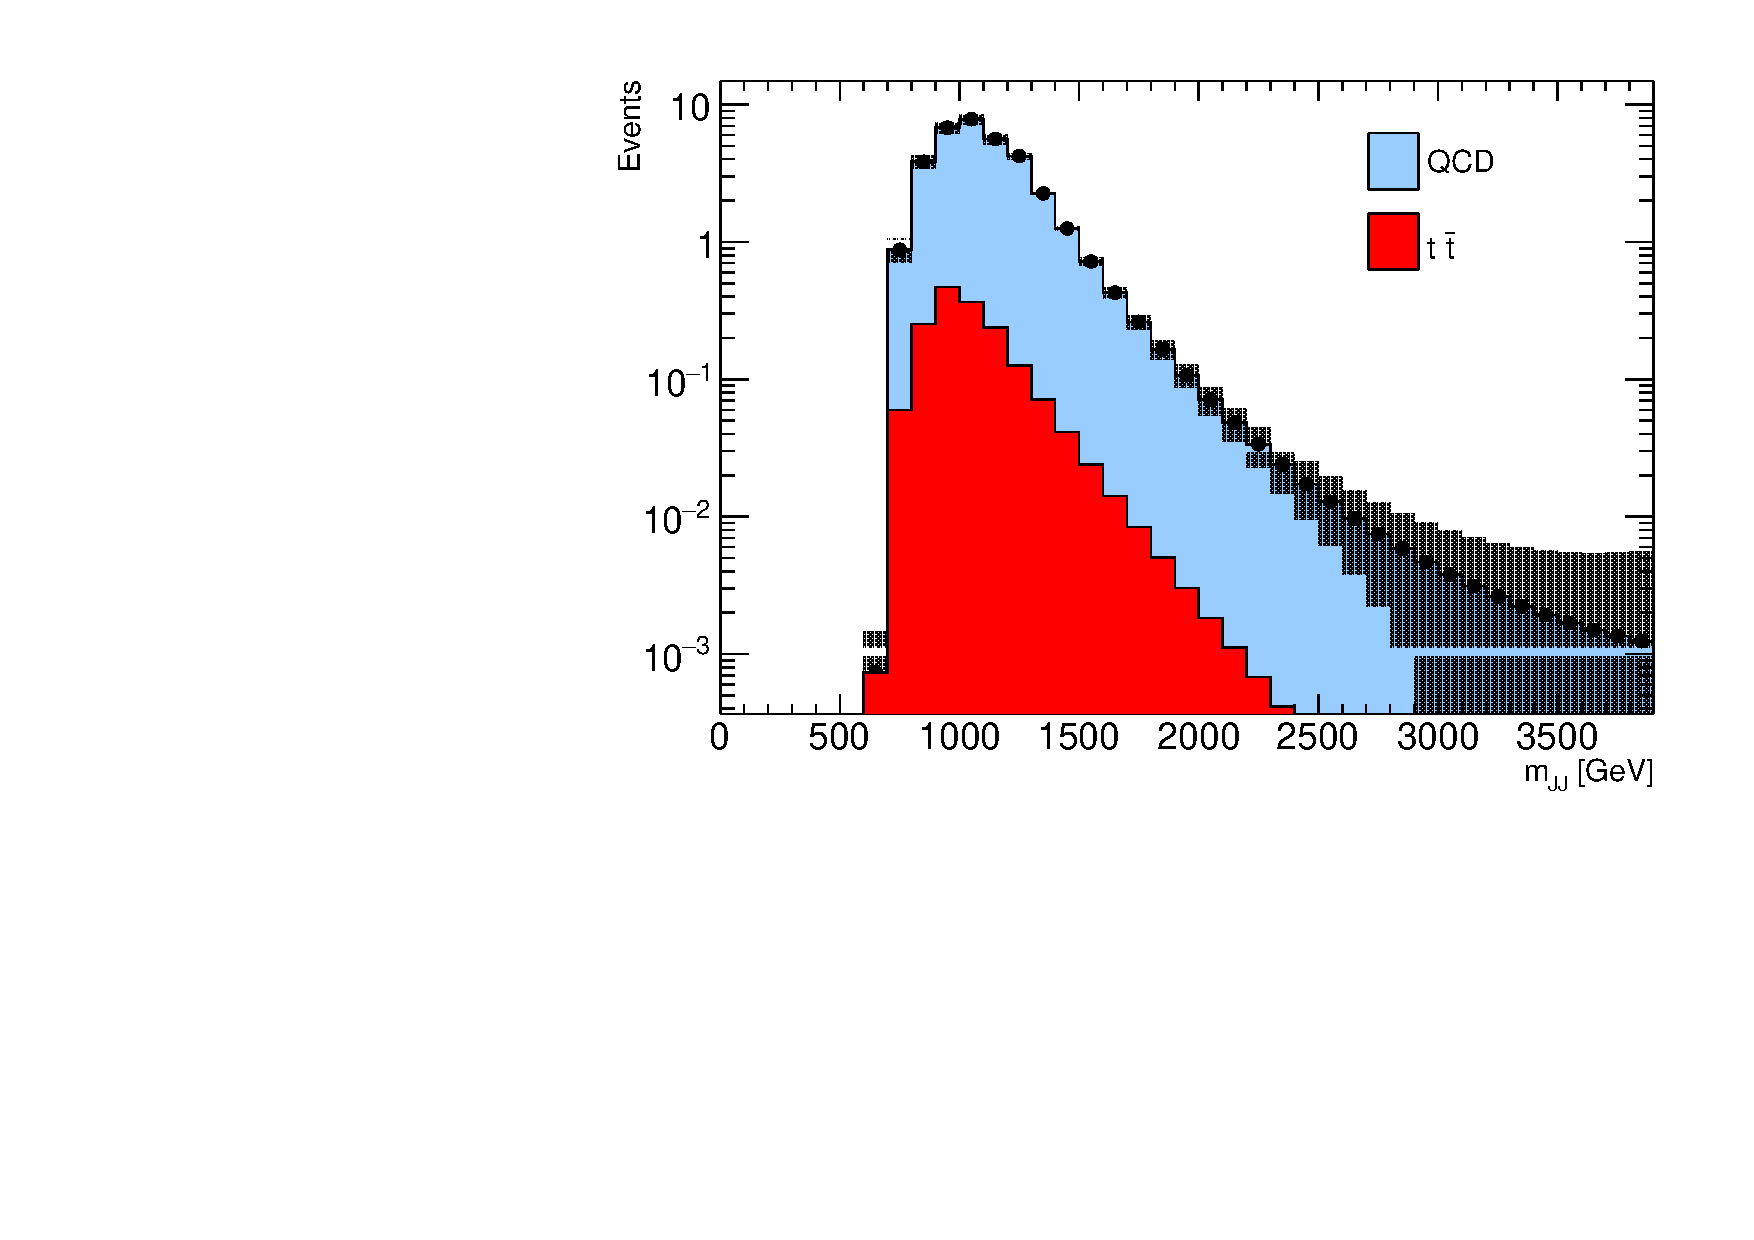
\includegraphics[width=0.45\textwidth,angle=-90]{figures/boosted/Smooth/FourTag_l_smoothed.pdf}\\
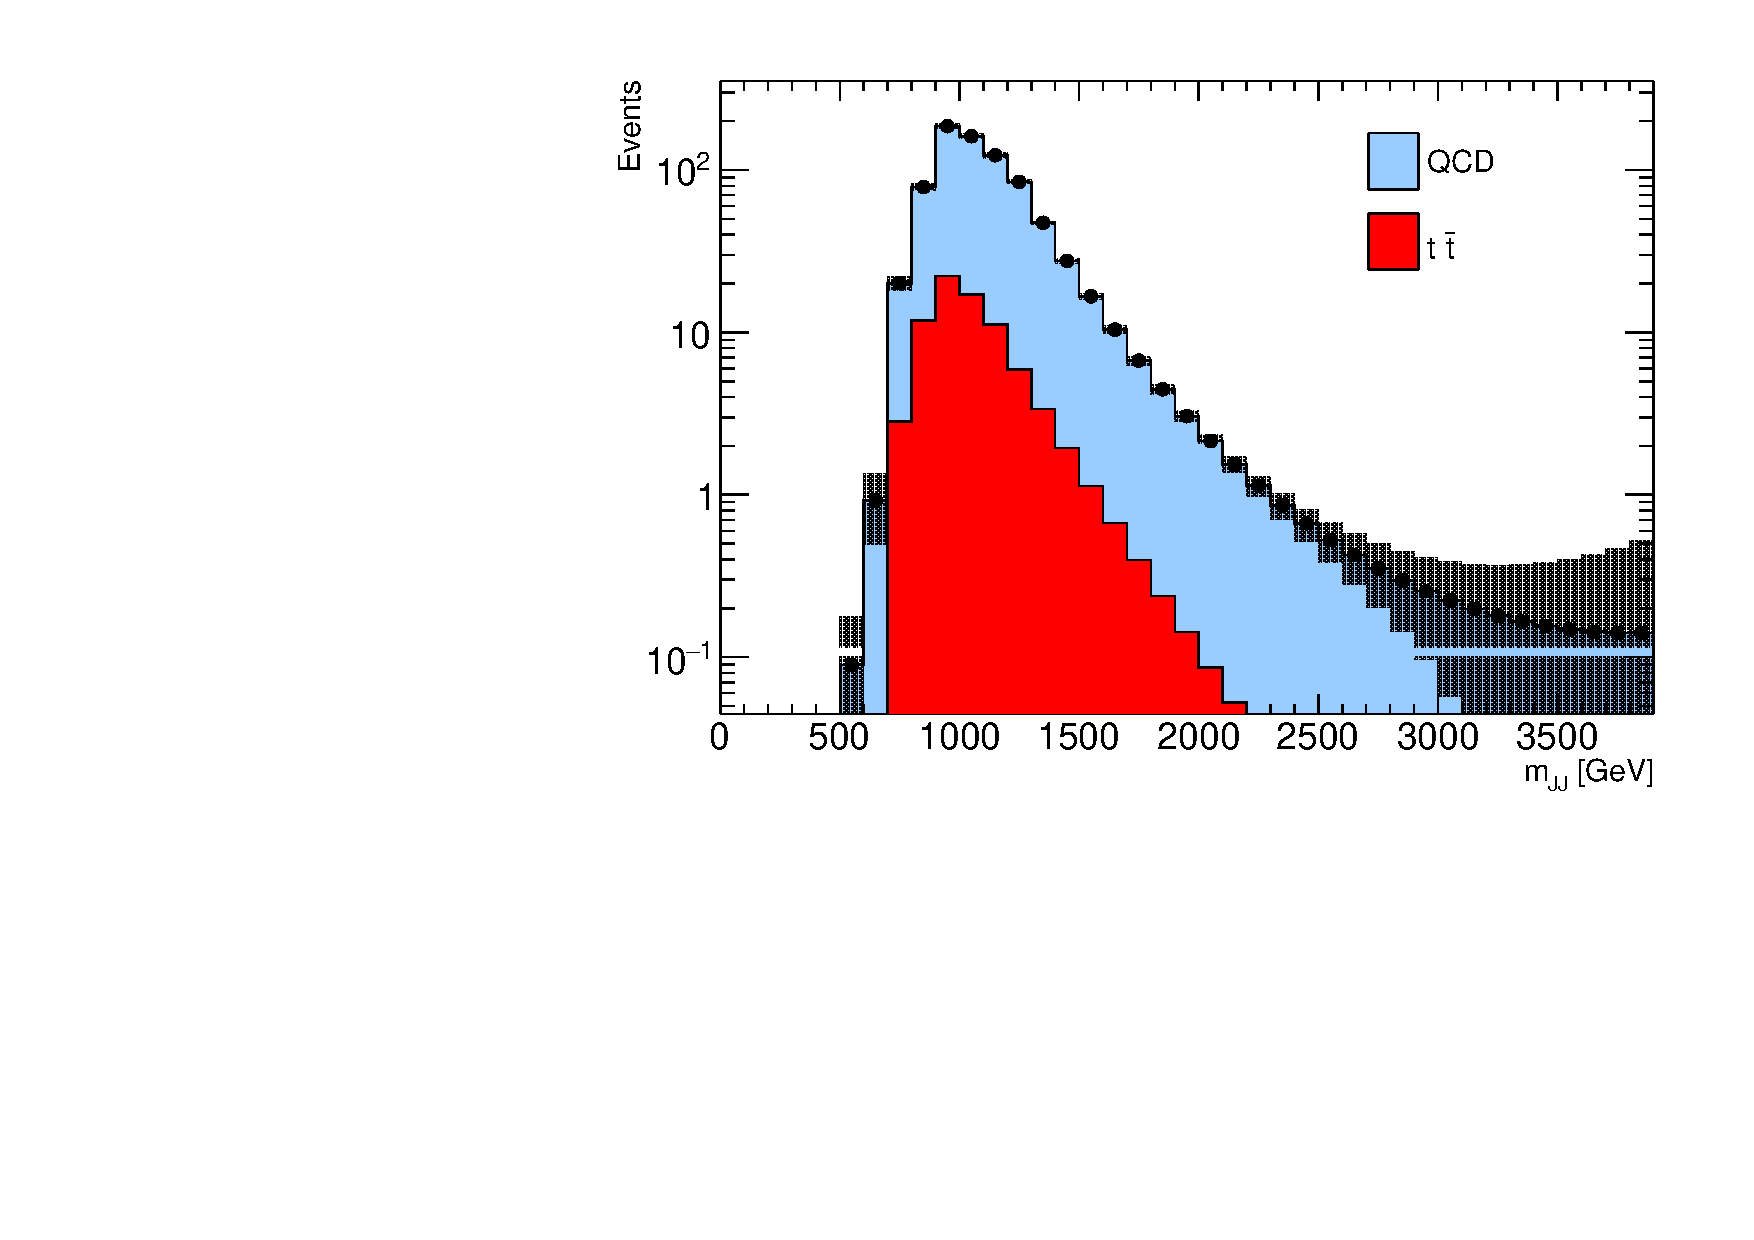
\includegraphics[width=0.45\textwidth,angle=-90]{figures/boosted/Smooth/ThreeTag_l_smoothed.pdf}\\
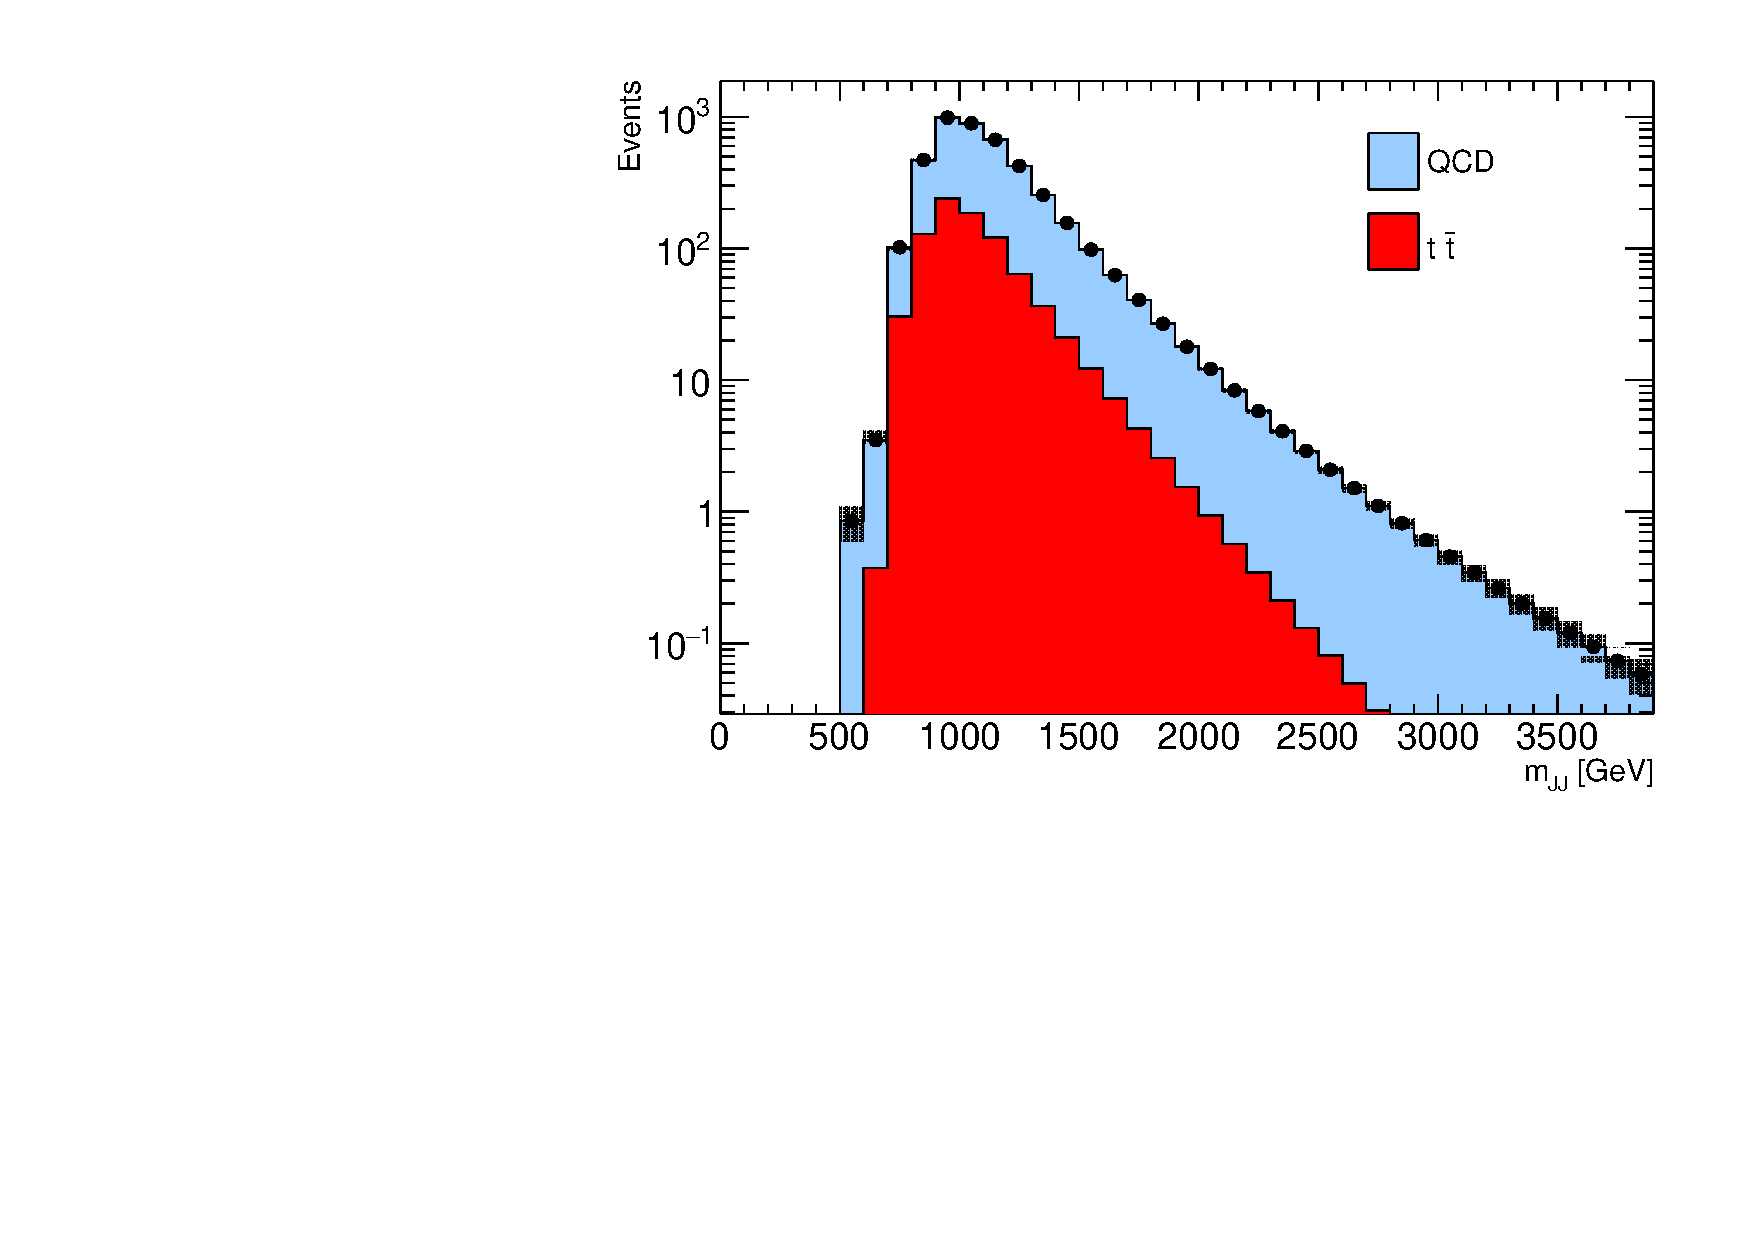
\includegraphics[width=0.45\textwidth,angle=-90]{figures/boosted/Smooth/TwoTag_split_l_smoothed.pdf}\\
\caption{Smoothed background estimations the $4b$ (top), $3b$ (middle), and $2bs$ (bottom) signal regions. Only smoothing statistical uncertainties are shown here. }
\label{fig:signal-region-smooth-bkg}
\end{center}
\end{figure}


%\begin{figure}[htbp!]
%\begin{center}
%   \includegraphics[width=0.45\textwidth,angle=-90]{figures/boosted/background/DrawCompleteBkgEst_DiJetMass_Pass4GoodTrackJetPass4b77PassSRMass_smoothed.pdf}
%   \includegraphics[width=0.45\textwidth,angle=-90]{figures/boosted/background/DrawCompleteBkgEst_DiJetMass_Pass4GoodTrackJetPass3b77PassSRMass_smoothed.pdf}
%\caption{Smoothed background estimations for the $4b$ (left) and $3b$ (right) signal regions. The uncertainty bands include all statistical and systematic uncertainties. \textbf{TO BE UPDATED} }
%\label{fig:signal-region-smooth-bkg-allSYS}
%\end{center}
%\end{figure}

\clearpage
\subsubsection{Scaled Dijet Mass Distribution in Signal region}
\label{sec:boosted-SR-mjjscaled}

%%\paragraph{}
As is done in the resolved analysis, we also consider the scaled $M_{JJ}$ distribution.  In this case, the two higgs candidate 4-vectors are scaled by $m_{h} / m_{J}$, where $m_h = 125$ GeV, and $m_{J}$ is the \largeR jet mass of the Higgs candidate.  While this distribution is expected to have less impact on the boosted analysis, because the mass correction is small relative to the signal masses being considered, we investigate this variable for possible improvements and for consistency with the resolved analysis. The scaled dijet mass distribution can be found in Figure~\ref{fig:signal-region-bkg-scaled}. Its impact of the boosted analysis limit can be found in Appendix~\ref{sec:app-optimization-polemass}.

%%\paragraph{}
For determining the choice of the final discriminant, both the expected limits on the nominal and scaled dijet mass distribution have been computed.  Since the scaled dijet  mass distribution based limits are consistent (slightly better at low mass and slightly worse at high mass, with differences of the order of 10\%) than the nominal dijet mass limits, we  proceed to use the scaled dijet mass distribution for consistency with the resolved analysis.

\begin{figure}[htbp!]
\begin{center}
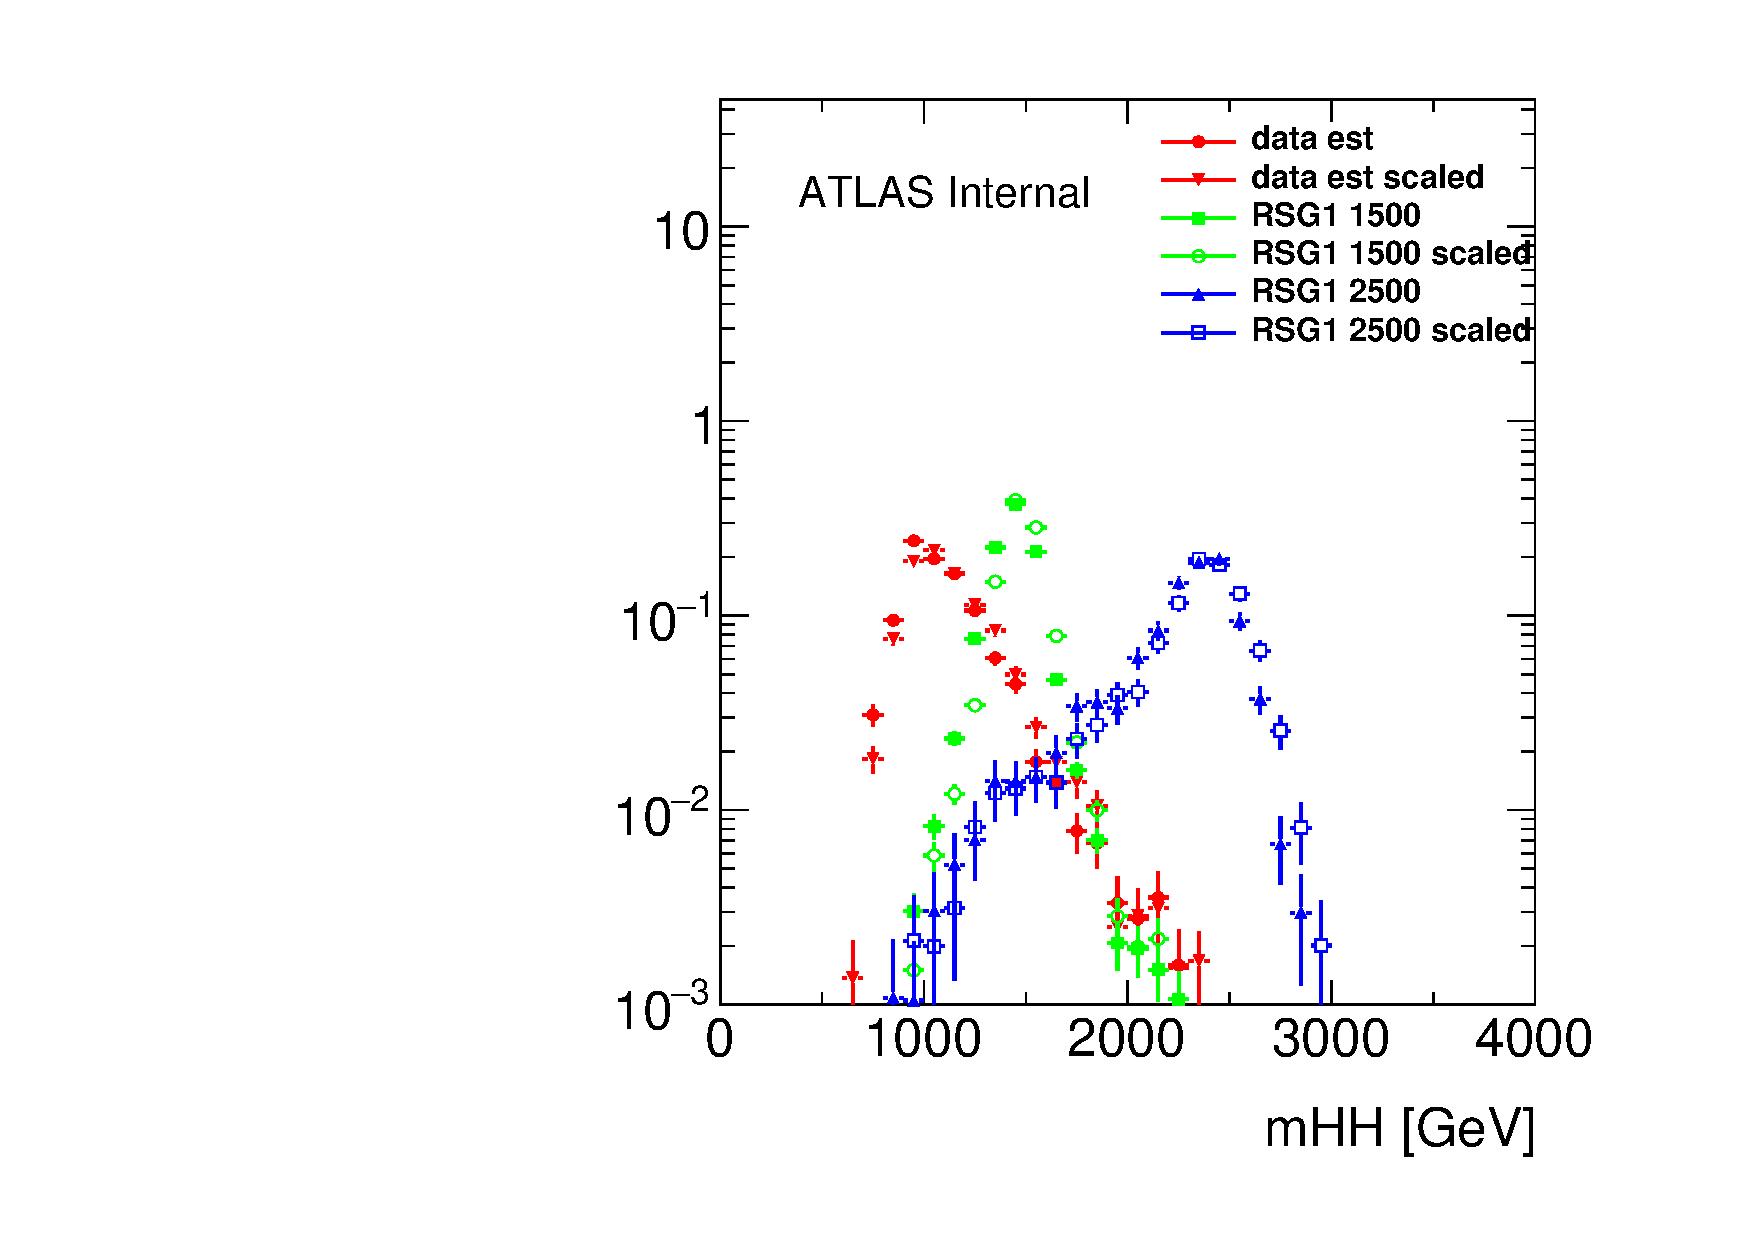
\includegraphics[width=0.45\textwidth,angle=-90]{figures/boosted/Other/FourTag_Signal_compare_scale_mHH_1.pdf}\\
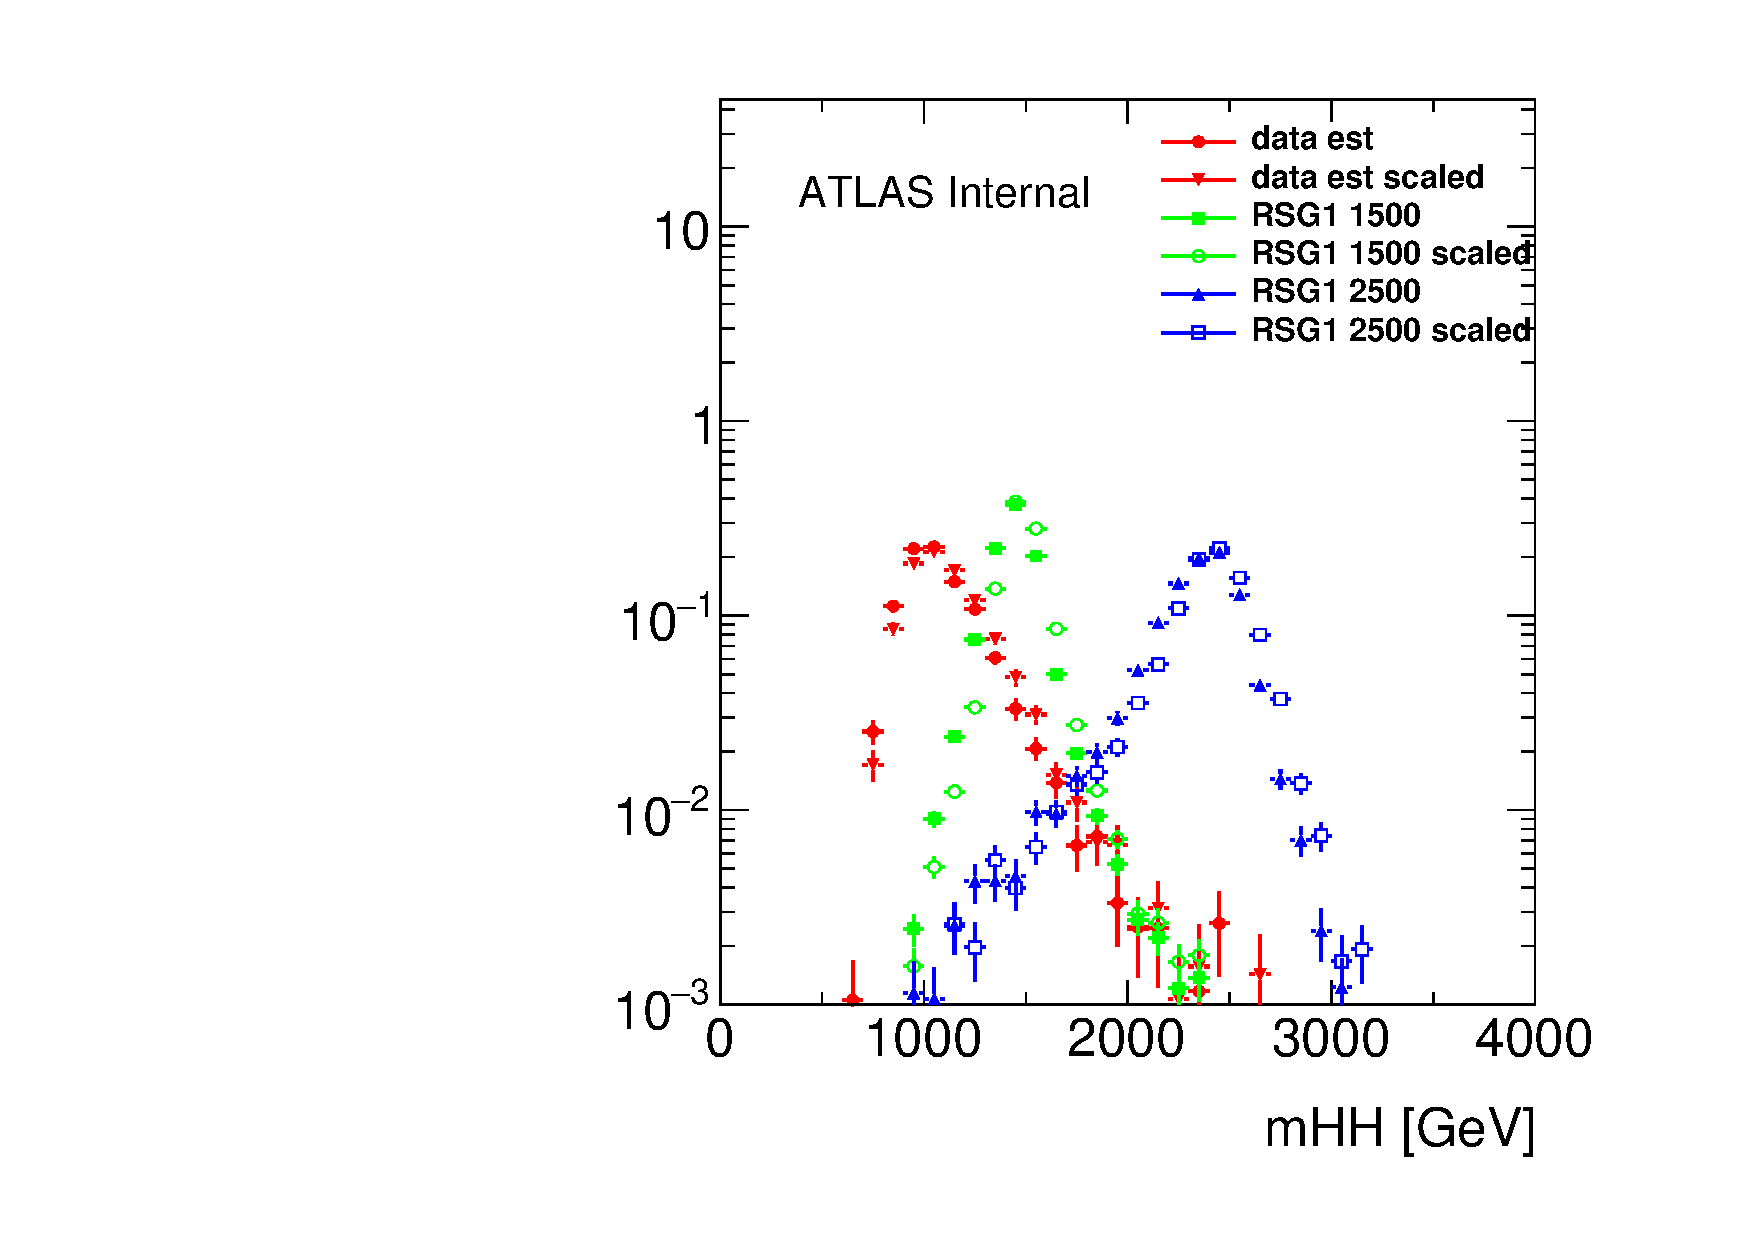
\includegraphics[width=0.45\textwidth,angle=-90]{figures/boosted/Other/ThreeTag_Signal_compare_scale_mHH_1.pdf}\\
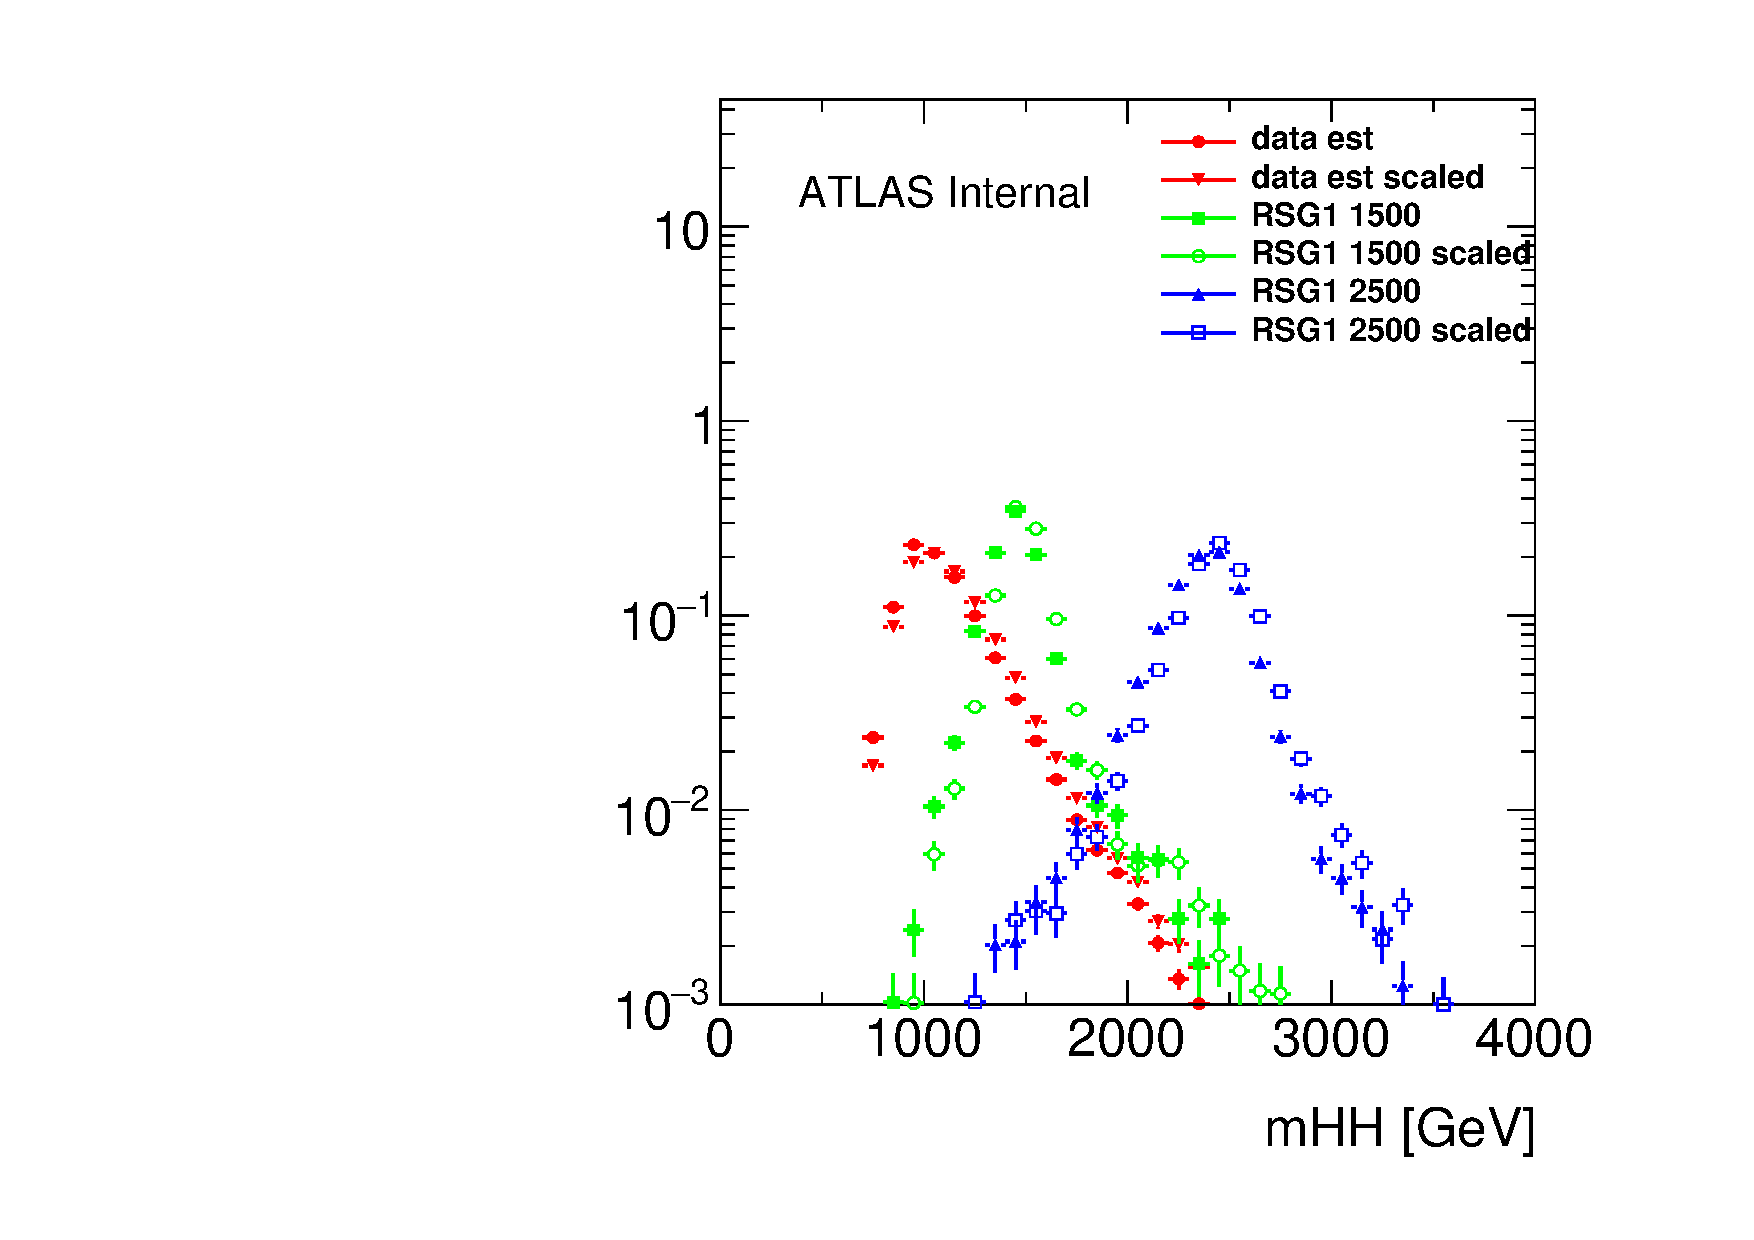
\includegraphics[width=0.45\textwidth,angle=-90]{figures/boosted/Other/TwoTag_split_Signal_compare_scale_mHH_1.pdf}
\caption{Normalized Scaled dijet mass distributions for the $4b$ (top), $3b$ (middle), and $2bs$ (bottom) signal regions.  For comparison, the unscaled distributions are shown on the same plot. }
\label{fig:signal-region-bkg-scaled}
\end{center}
\end{figure}

%%\paragraph{}
As is done for the dijet mass distribution,  the scaled dijet mass distribution is smoothed. The smoothing is performed between 1200 GeV and 3000 GeV for the QCD  and $t\bar{t}$. The smoothed distributions can be seen in Figures~\ref{fig:signal-region-mjjscaled-4b-smoothing}, ~\ref{fig:signal-region-mjjscaled-3b-smoothing}, and~\ref{fig:signal-region-mjjscaled-2bs-smoothing}. The values of the estimated fit parameters in the $4b$ and $3b$ and $2bs$ signal regions can be found in Table~\ref{tab:smoothparams_pole}.

%%\paragraph{}
The final signal region prediction, using scaled di-jet mass distribution, with only statistical uncertainties, are shown in Figure~\ref{fig:signal-region-mjjscaled-nonsmooth-bkg-noSYS}(Figure~\ref{fig:signal-region-mjjscaled-smooth-bkg-noSYS}) as before(after) smoothing.

\begin{table}[htbp!]
\begin{center}
\begin{footnotesize} 
\begin{tabular}{c|c|c|c|c|c|c} 
Region & $ a_{t\bar{t}}$ & $ b_{t\bar{t}}$ & $ c_{t\bar{t}}$ & $ a_{qcd}$ & $ b_{qcd}$ & $c_{qcd}$ \\ 
\hline\hline 
& & & & & &\\ 
FourTag & -2.02 $\pm$ 1.17 & 42.46 $\pm$ 9.87 & 1.31 $\pm$ 8.98 & -0.49 $\pm$ 1.59 & 53.06 $\pm$ 15.2 & -11.1 $\pm$ 12.8\\ 
ThreeTag & 1.84 $\pm$ 1.17 & 42.45 $\pm$ 9.88 & 1.32 $\pm$ 8.98 & 8.51 $\pm$ 0.98 & -13.8 $\pm$ 9.14 & 42.58 $\pm$ 7.87\\ 
TwoTag split & 4.22 $\pm$ 1.17 & 42.45 $\pm$ 9.88 & 1.32 $\pm$ 8.98 & 7.06 $\pm$ 0.32 & 11.54 $\pm$ 2.77 & 19.05 $\pm$ 2.48\\ 
& & & & & &\\ 
\hline\hline 
\end{tabular} 
\end{footnotesize} 
\newline 

\caption{Smoothing parameters in $4b$ and $3b$ and $2bs$ signal regions for scaled mass distributions, the correlation between parameters is almost always 0.99.}
\label{tab:smoothparams_pole}
\end{center}
\end{table}


\begin{figure}[htbp!]
\begin{center}
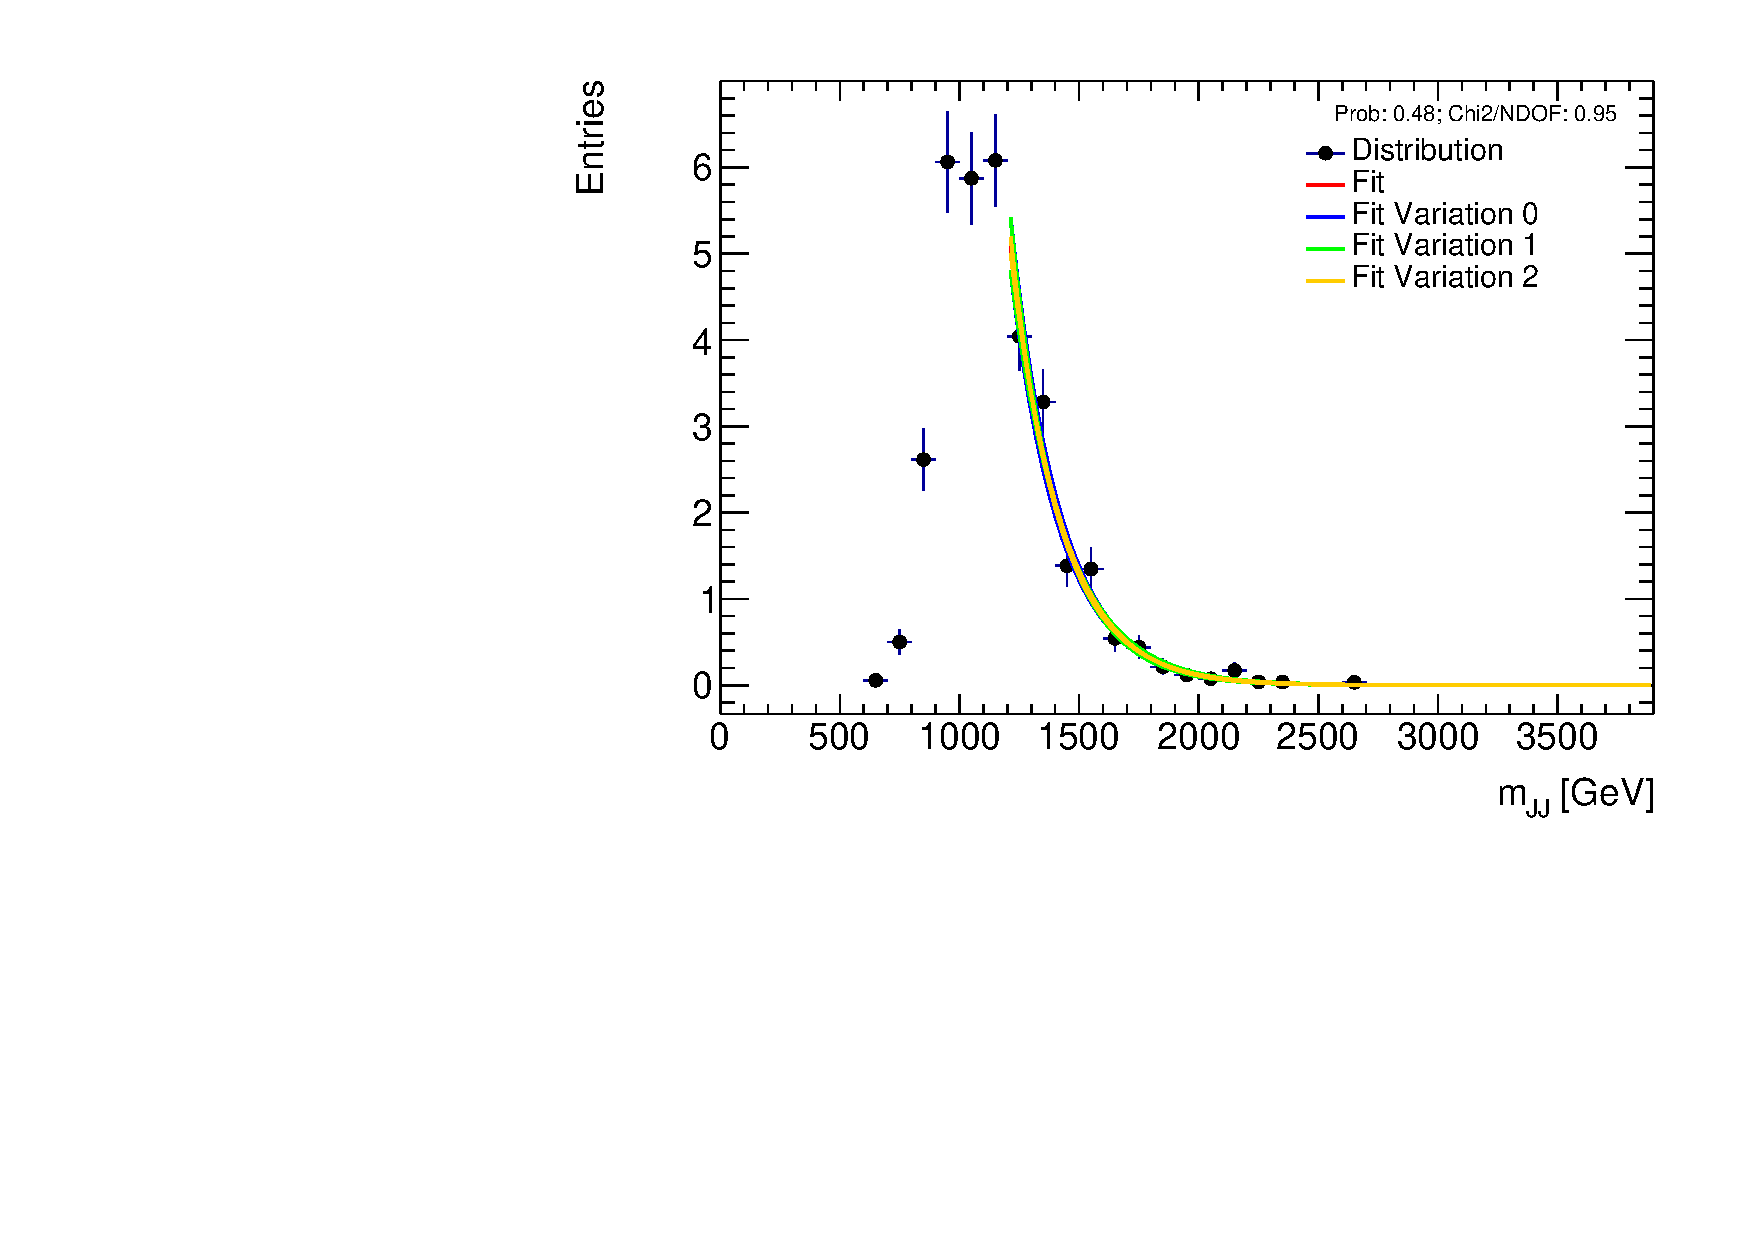
\includegraphics[width=0.45\textwidth,angle=-90]{figures/boosted/Smooth/qcd_est_FourTag_Signal_mHH_pole.pdf}
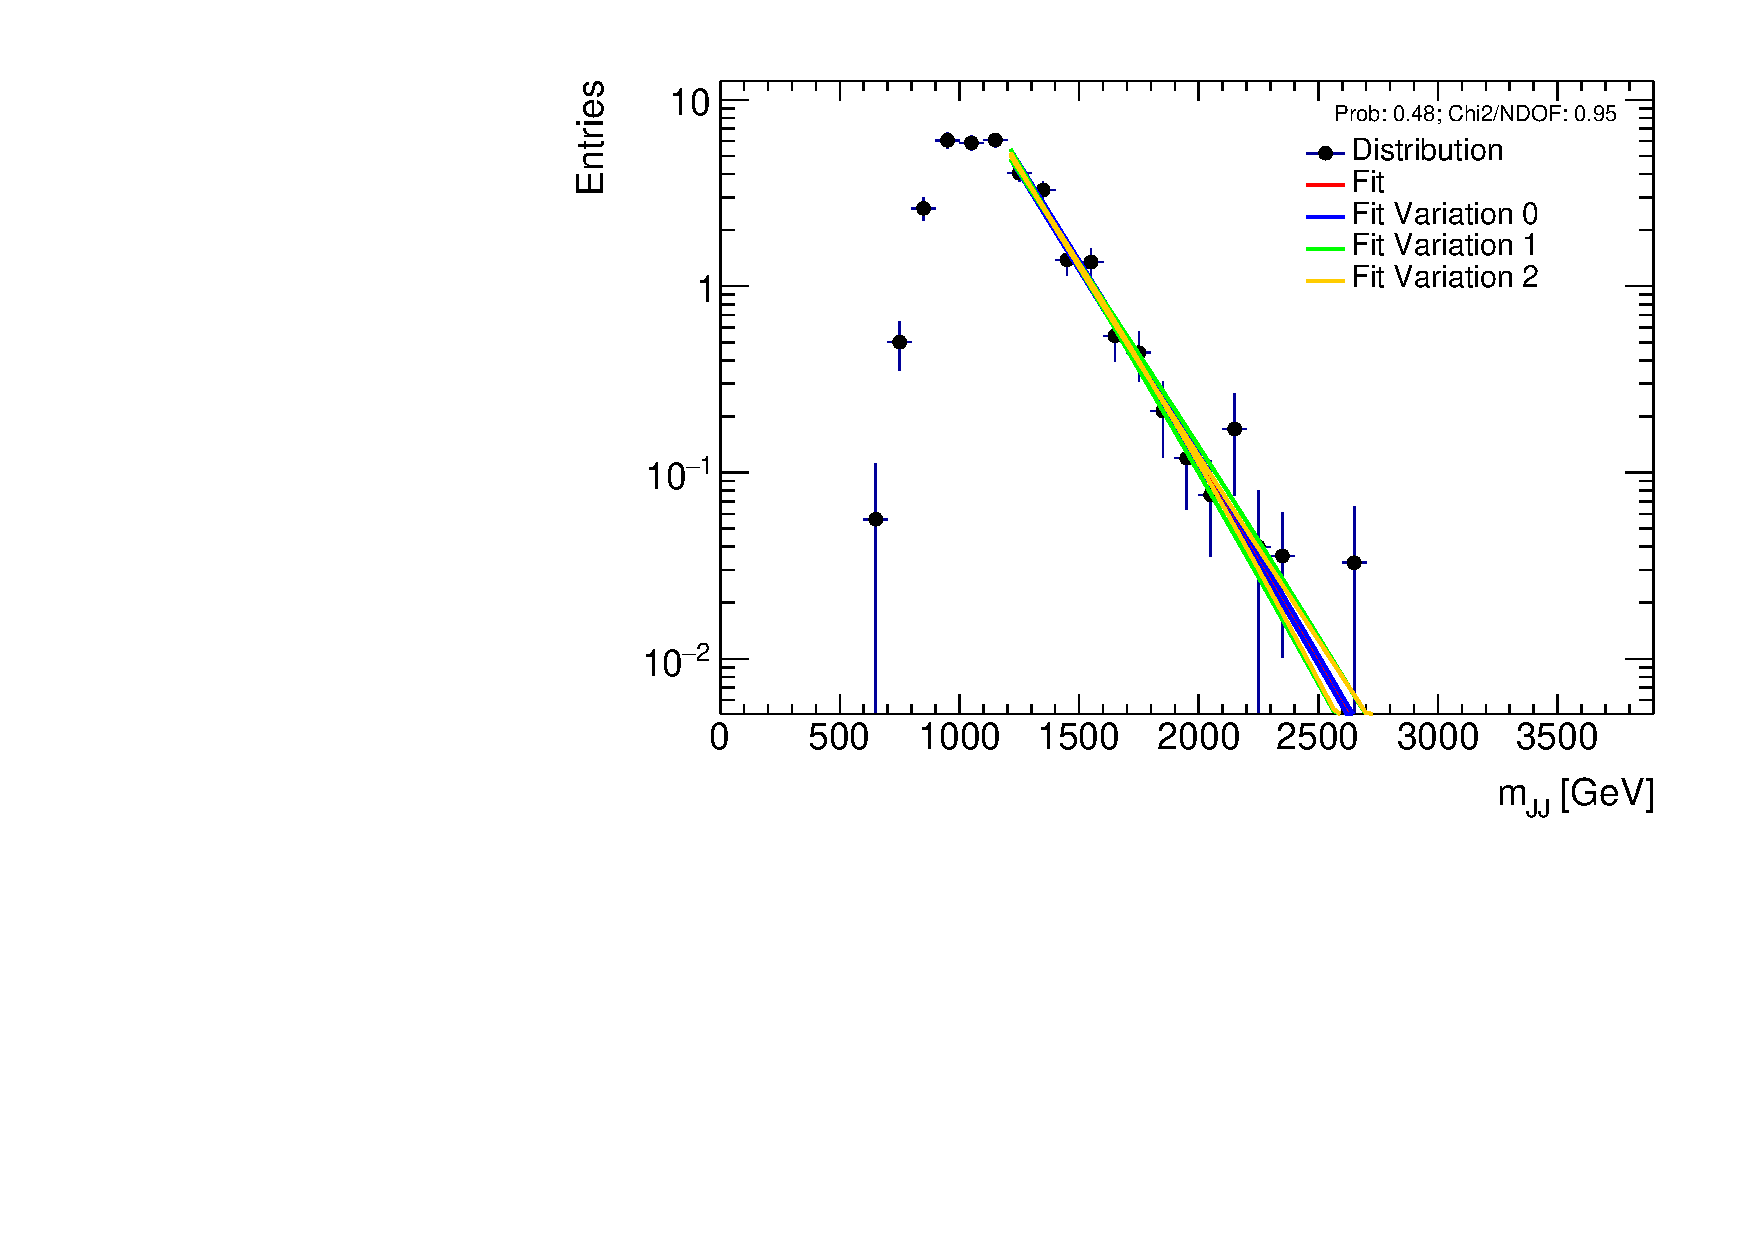
\includegraphics[width=0.45\textwidth,angle=-90]{figures/boosted/Smooth/qcd_est_FourTag_Signal_mHH_pole_l.pdf}\\
%   
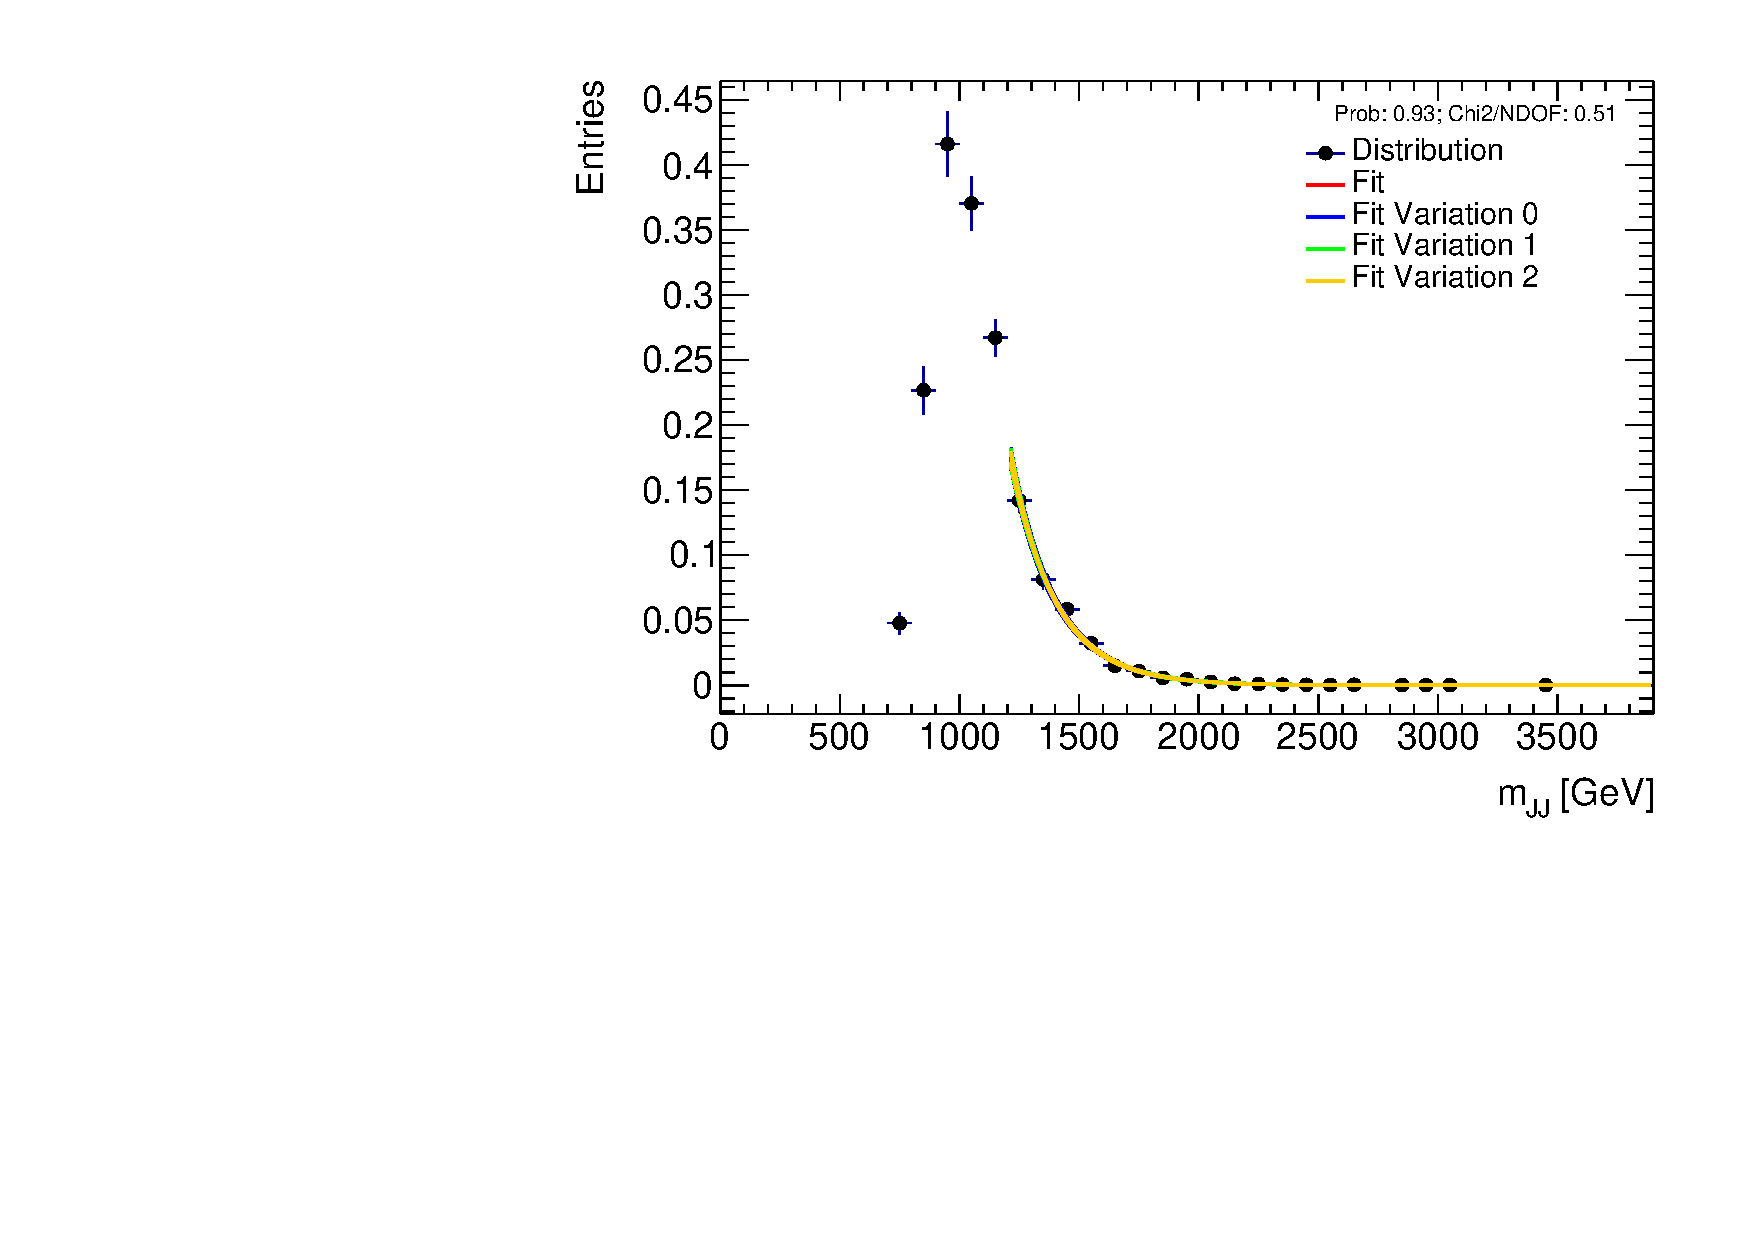
\includegraphics[width=0.45\textwidth,angle=-90]{figures/boosted/Smooth/ttbar_est_FourTag_Signal_mHH_pole.pdf}
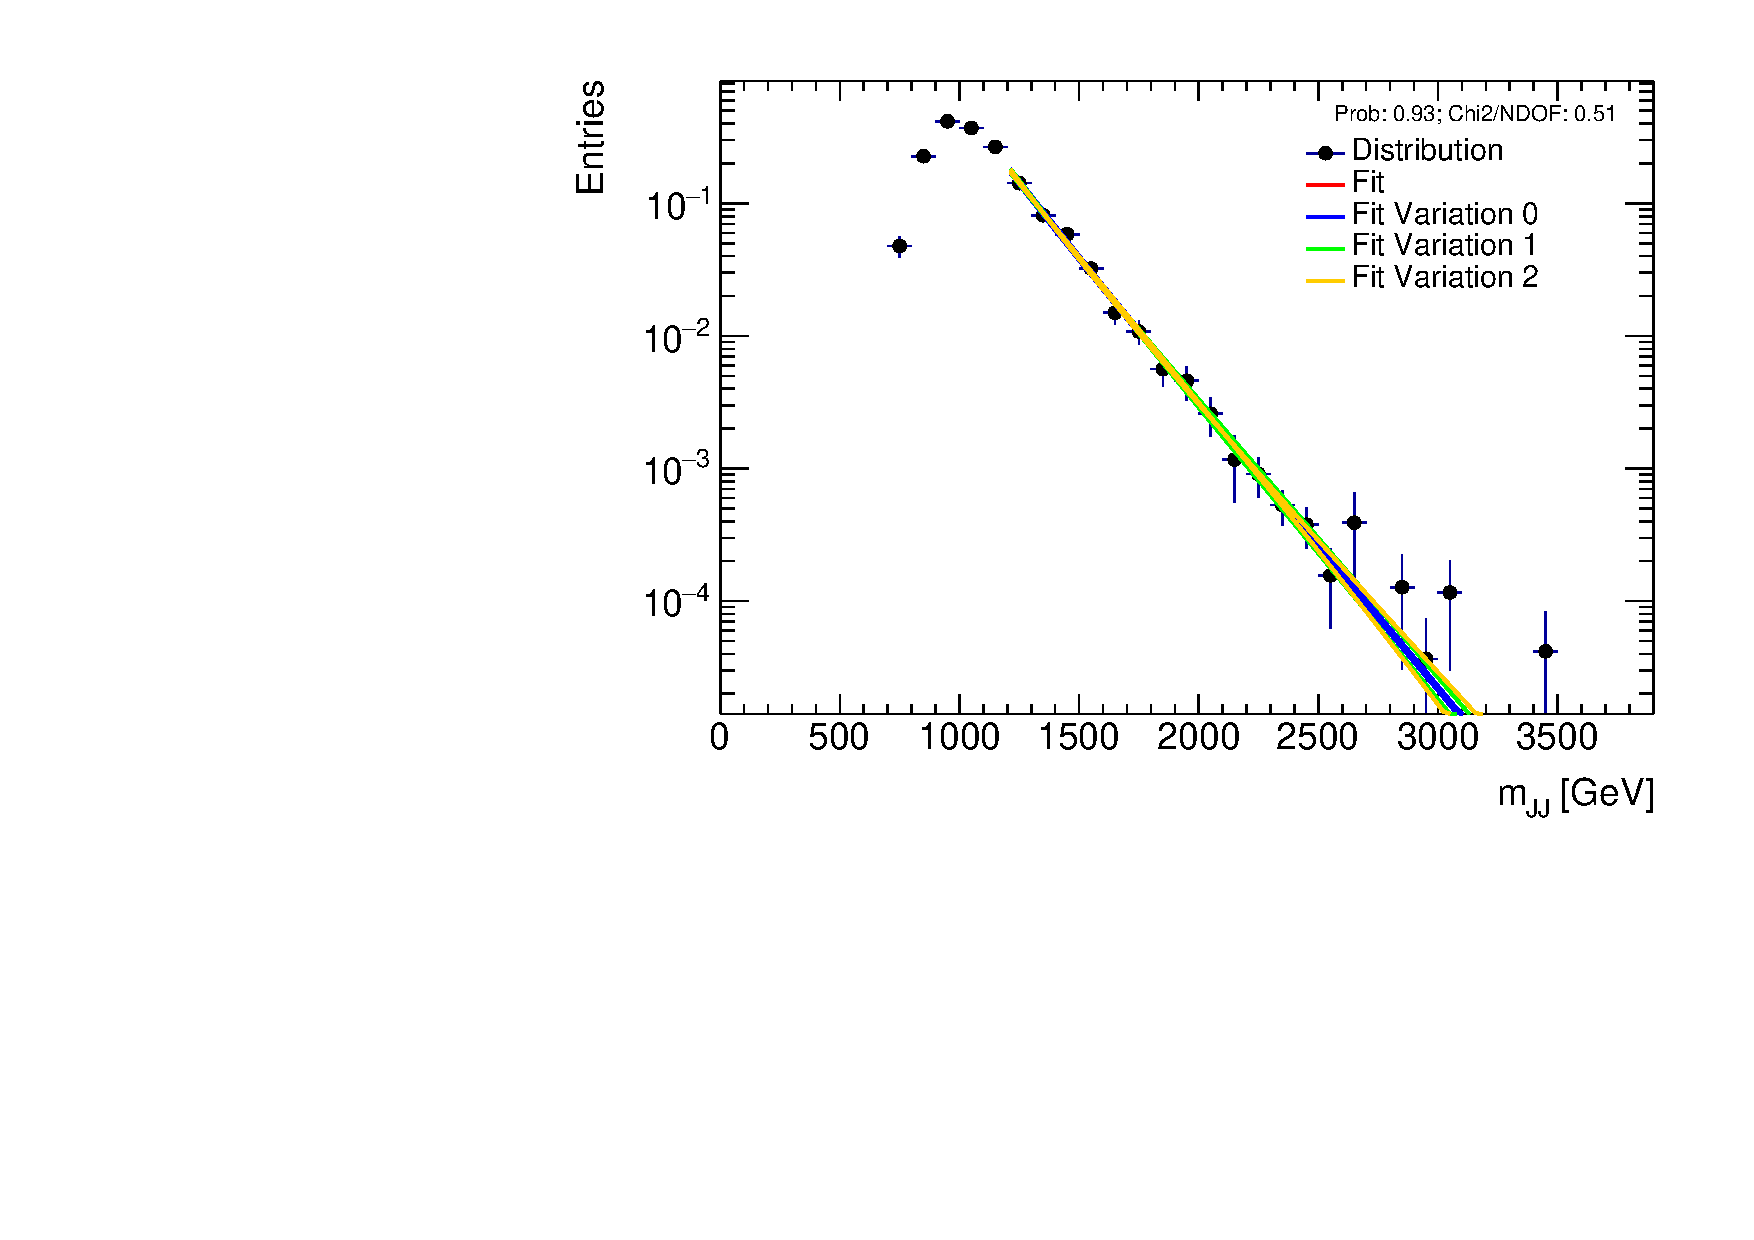
\includegraphics[width=0.45\textwidth,angle=-90]{figures/boosted/Smooth/ttbar_est_FourTag_Signal_mHH_pole_l.pdf}\\
\caption{Fits for scaled background smoothing are shown for QCD (top row) and $t\bar{t}$ (bottom row) in the $4b$ signal region.  The left figures show the distributions with linear $y$-axis scale along with the fit central value and variations. The right figures show the  distributions with log $y$-axis scale along with the fit central value and the fit variations as determined by the varying the fit parameters within uncertainties whilst taking into account parameter correlations. }
\label{fig:signal-region-mjjscaled-4b-smoothing}
\end{center}
\end{figure}

\begin{figure}[htbp!]
\begin{center}
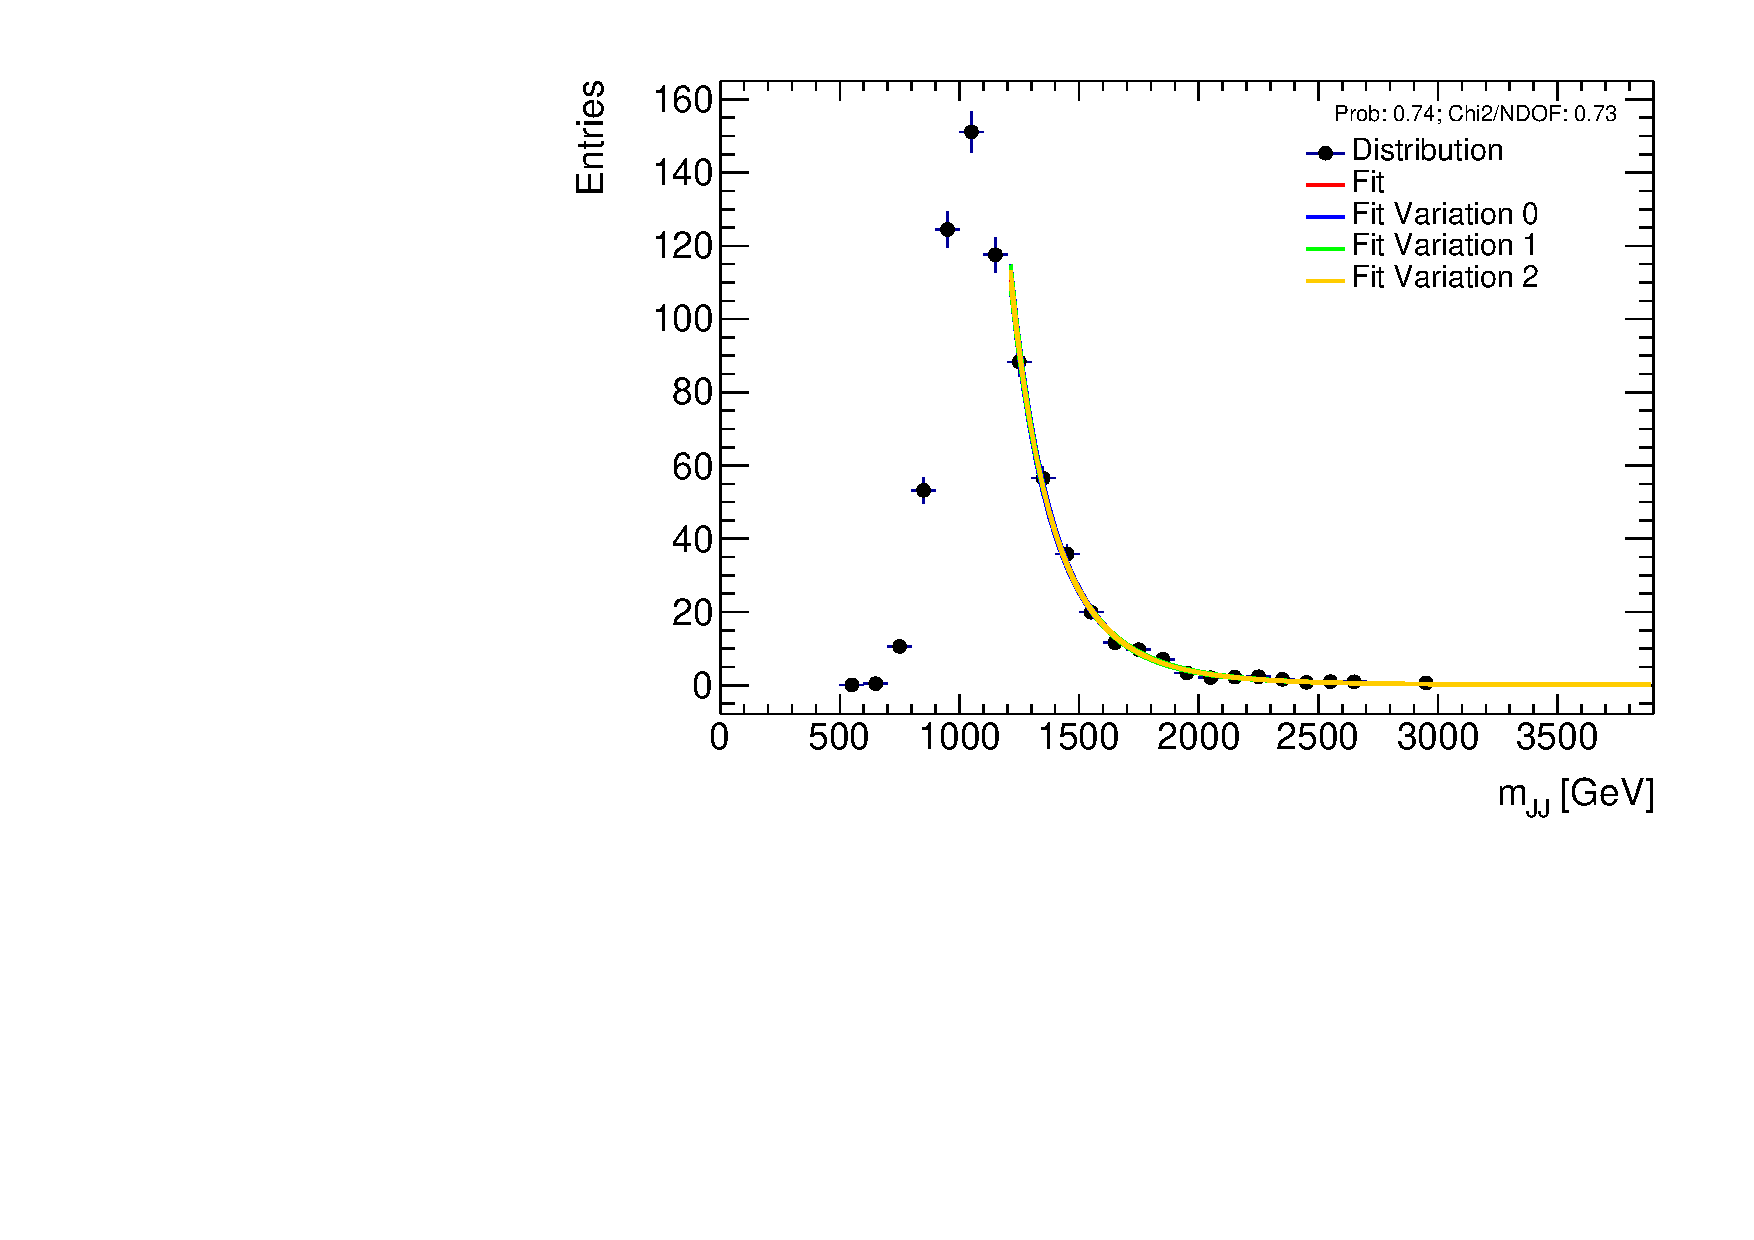
\includegraphics[width=0.45\textwidth,angle=-90]{figures/boosted/Smooth/qcd_est_ThreeTag_Signal_mHH_pole.pdf}
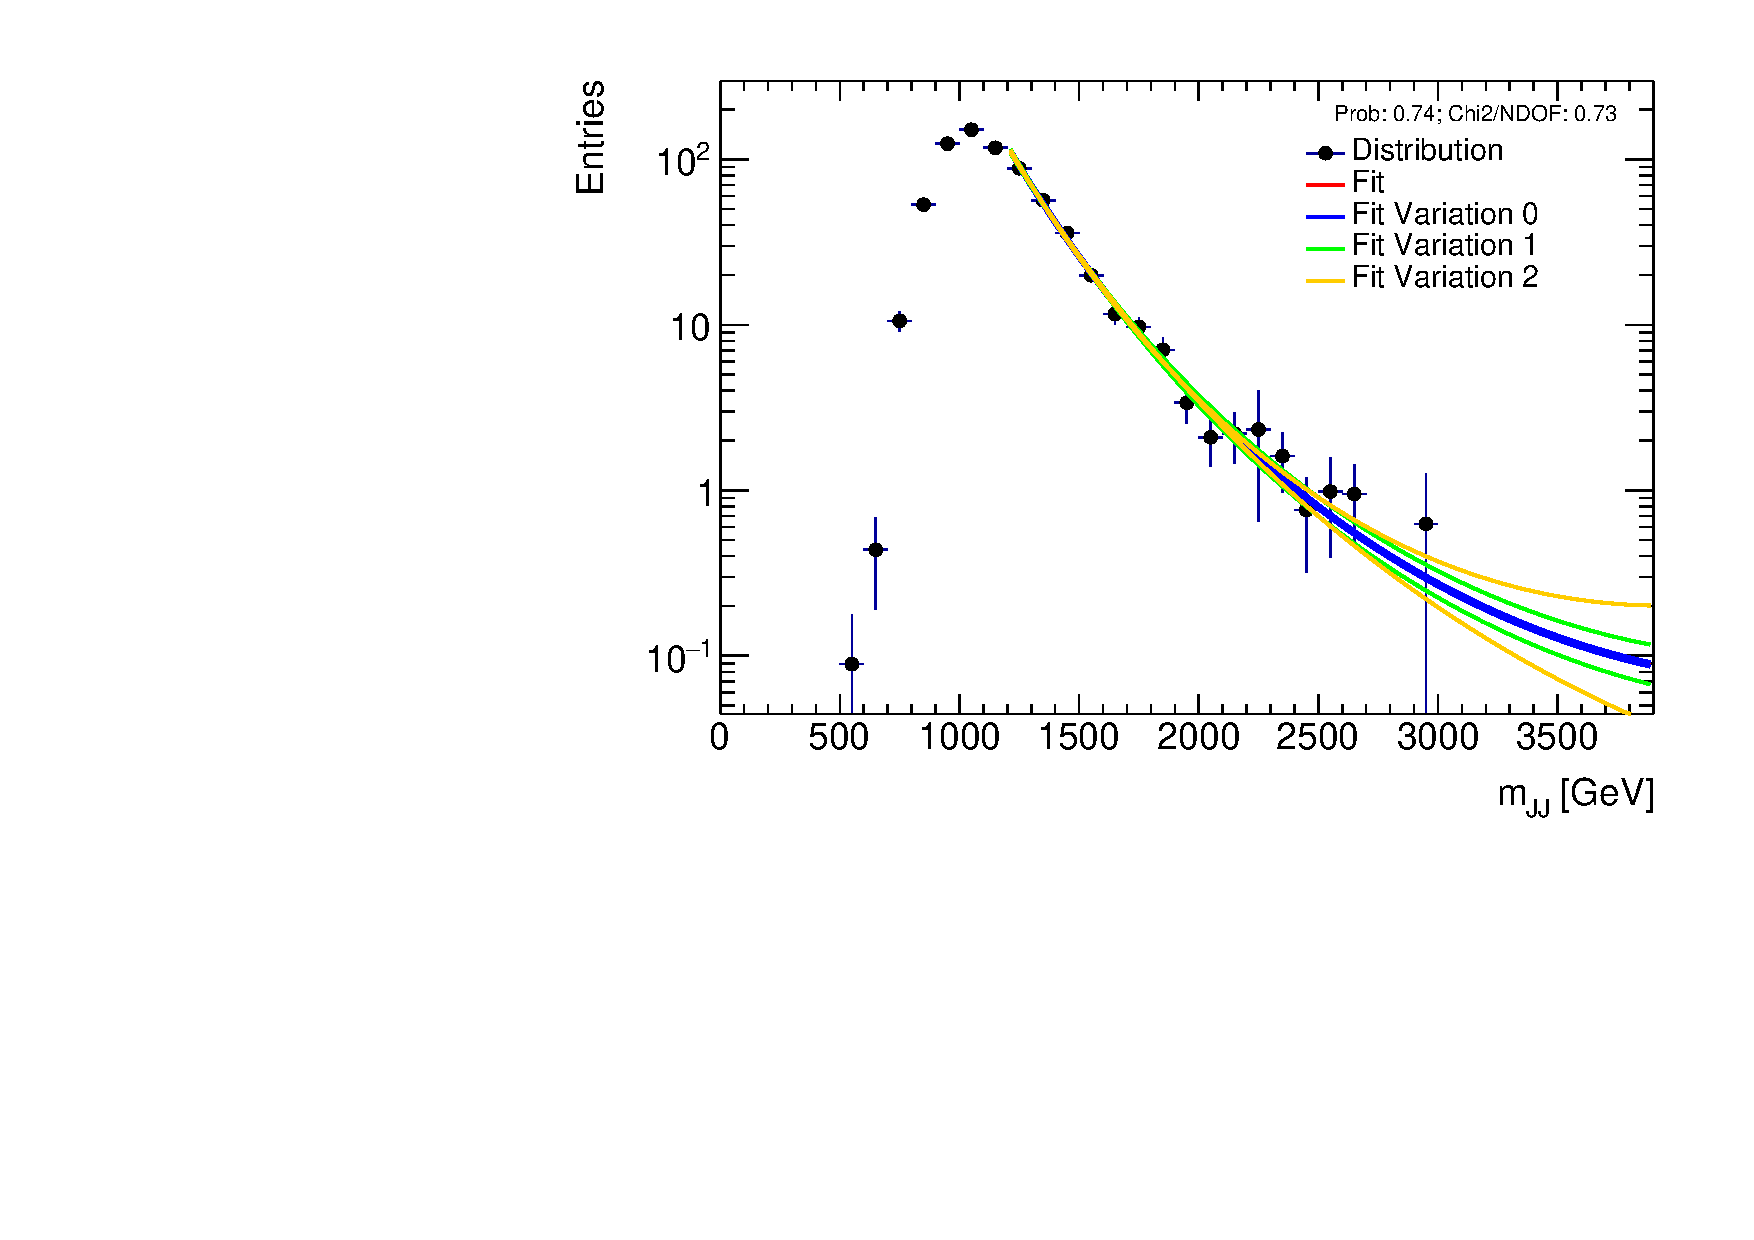
\includegraphics[width=0.45\textwidth,angle=-90]{figures/boosted/Smooth/qcd_est_ThreeTag_Signal_mHH_pole_l.pdf}\\
%   
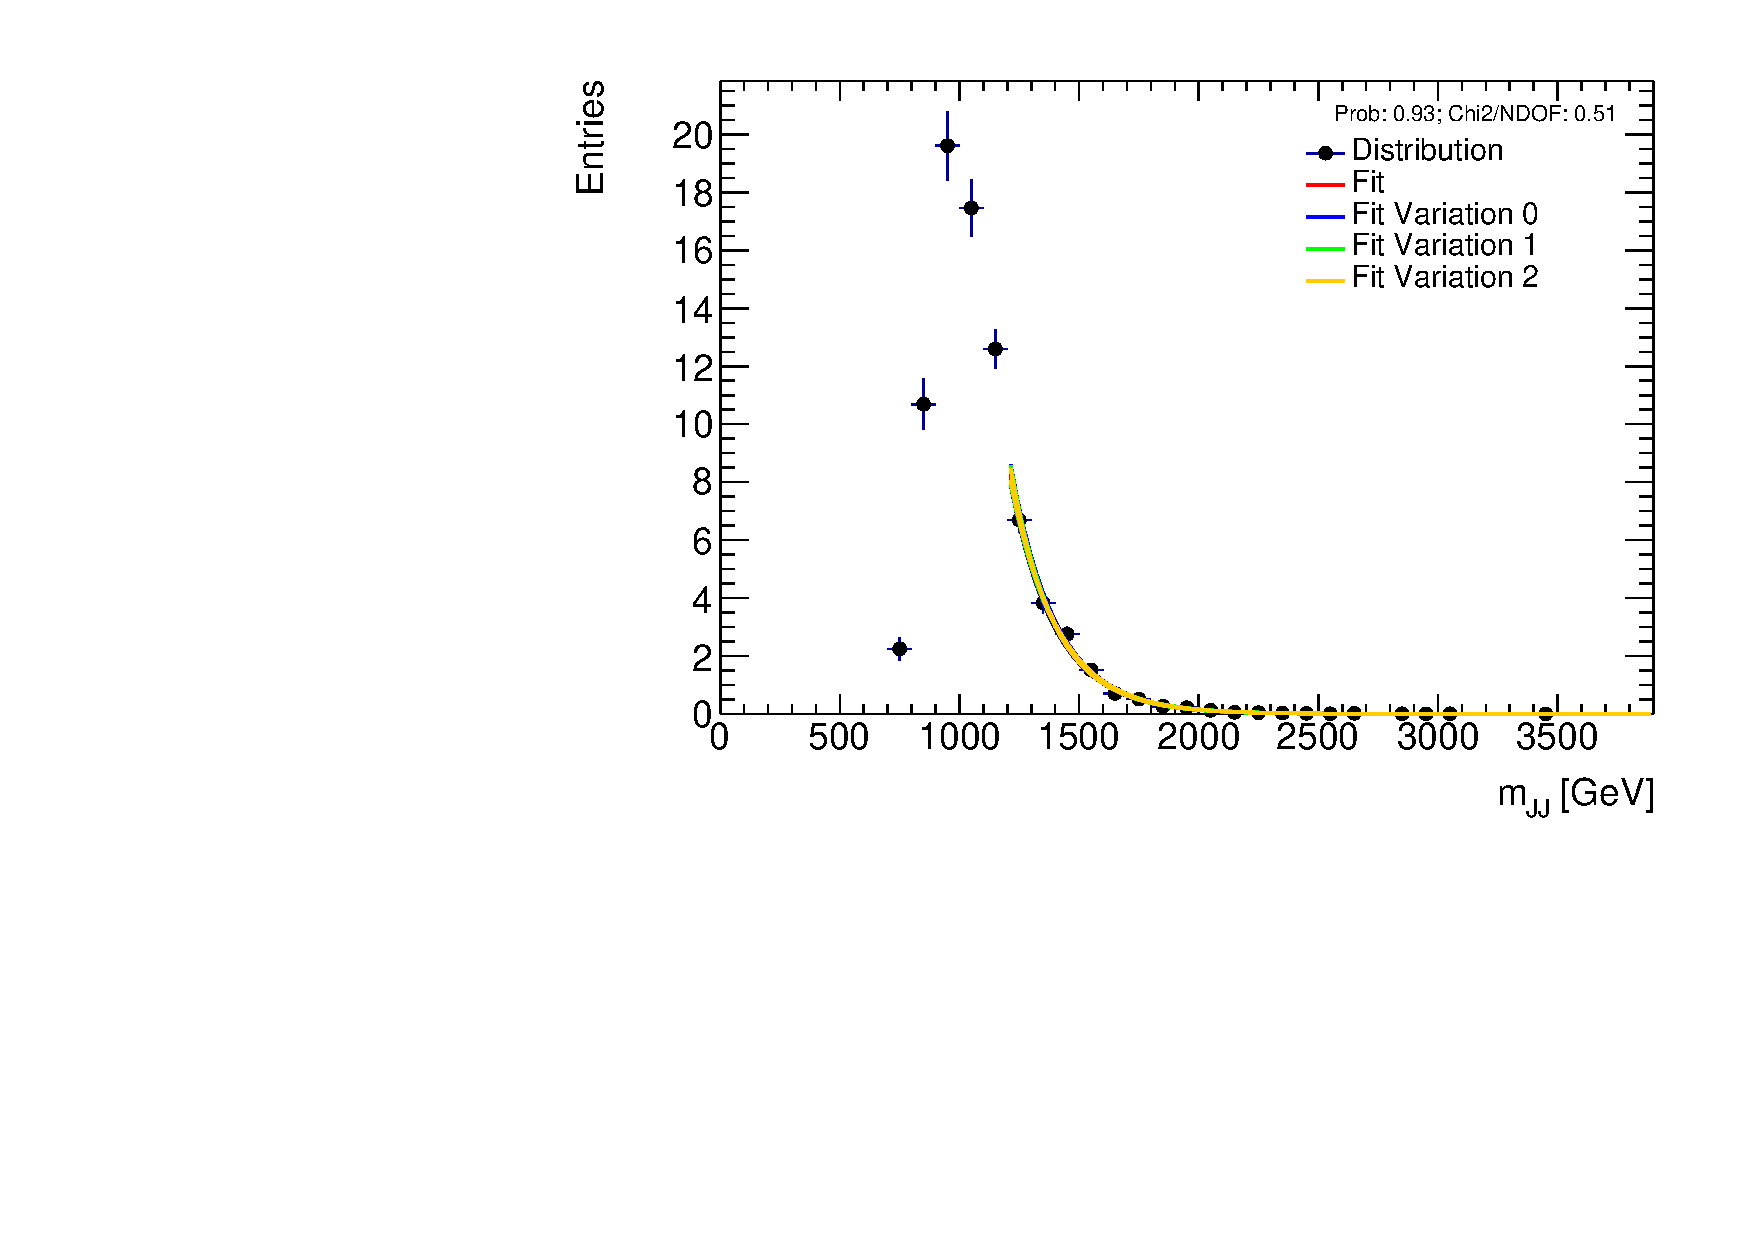
\includegraphics[width=0.45\textwidth,angle=-90]{figures/boosted/Smooth/ttbar_est_ThreeTag_Signal_mHH_pole.pdf}
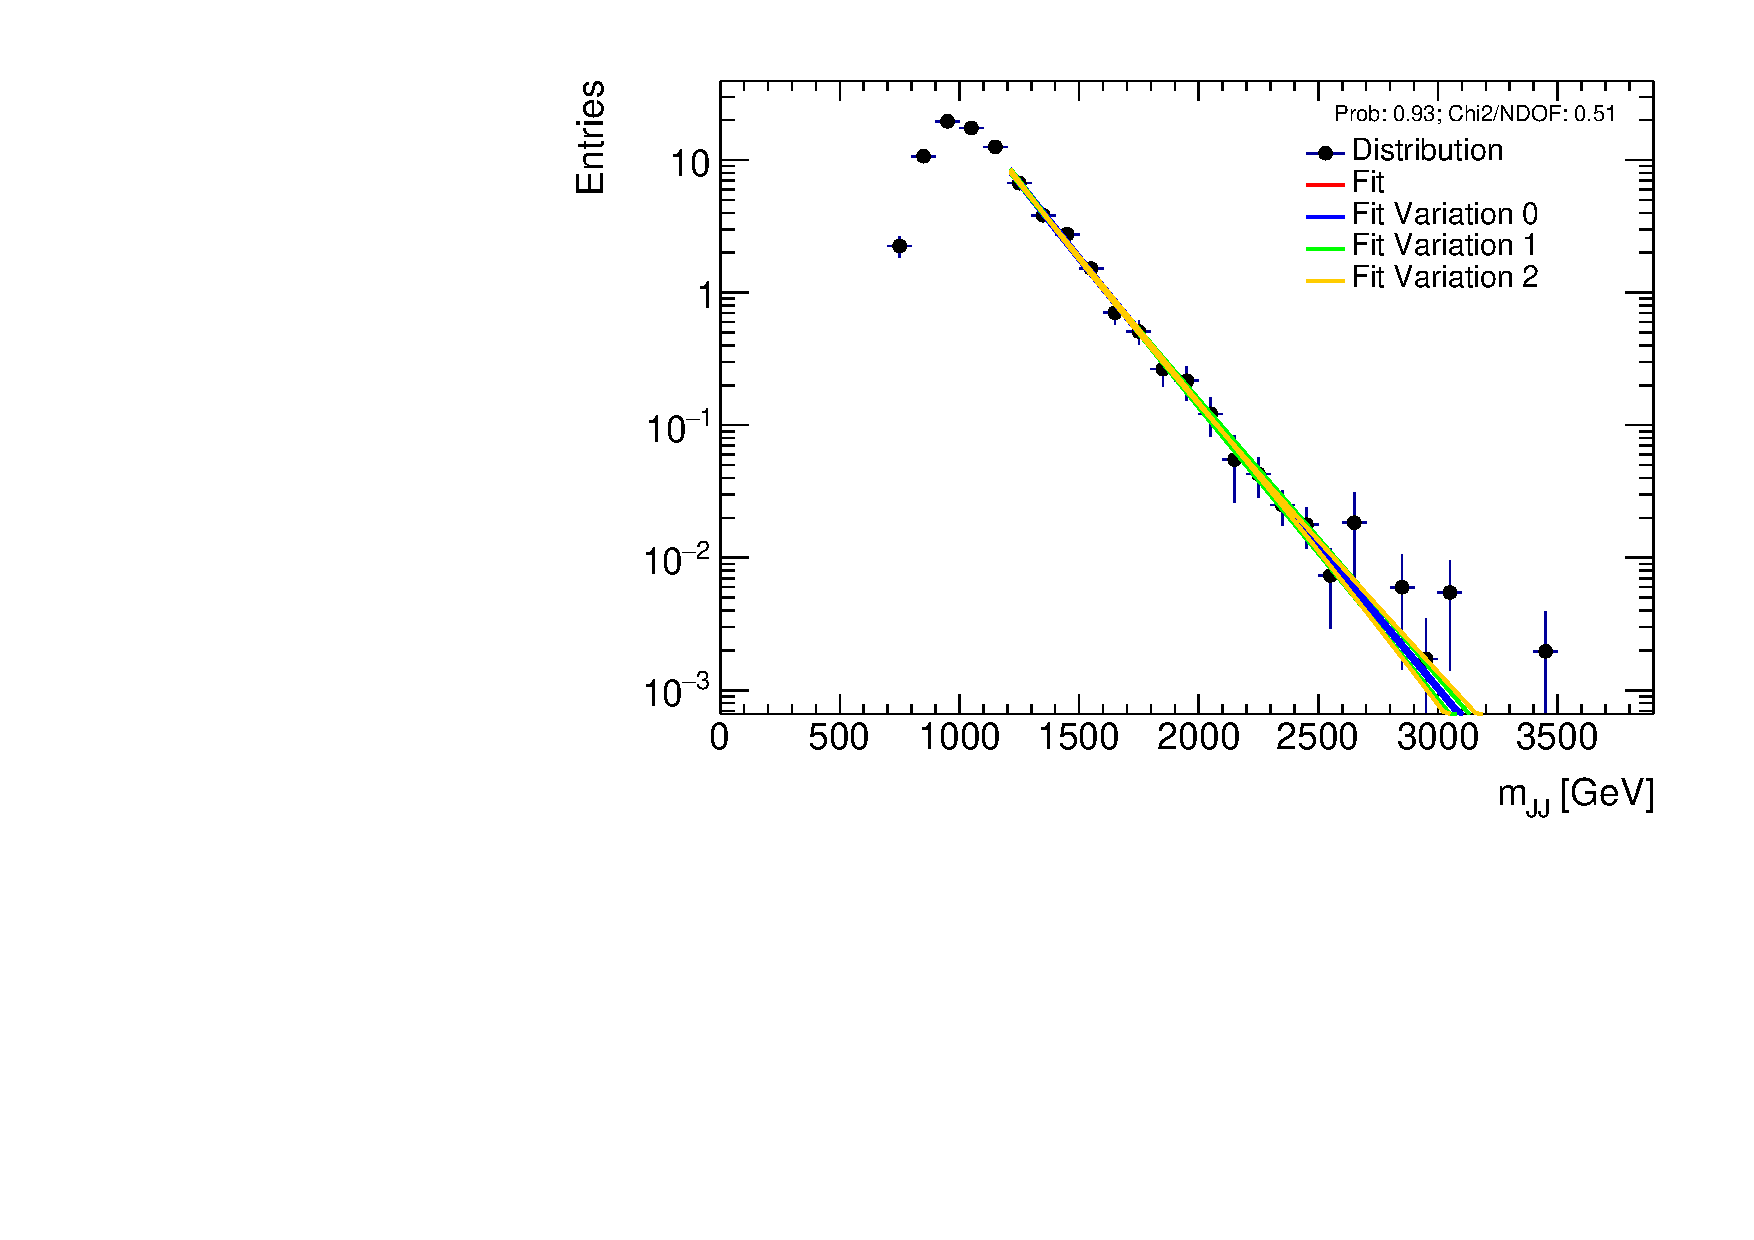
\includegraphics[width=0.45\textwidth,angle=-90]{figures/boosted/Smooth/ttbar_est_ThreeTag_Signal_mHH_pole_l.pdf}\\
\caption{Fits for scaled background smoothing are shown for QCD (top row) and $t\bar{t}$ (bottom row) in the $3b$ signal region.  The left figures show the distributions with linear $y$-axis scale along with the fit central value and variations. The right figures show the  distributions with log $y$-axis scale along with the fit central value and the fit variations as determined by the varying the fit parameters within uncertainties whilst taking into account parameter correlations. }
\label{fig:signal-region-mjjscaled-3b-smoothing}
\end{center}
\end{figure}

\begin{figure}[htbp!]
\begin{center}
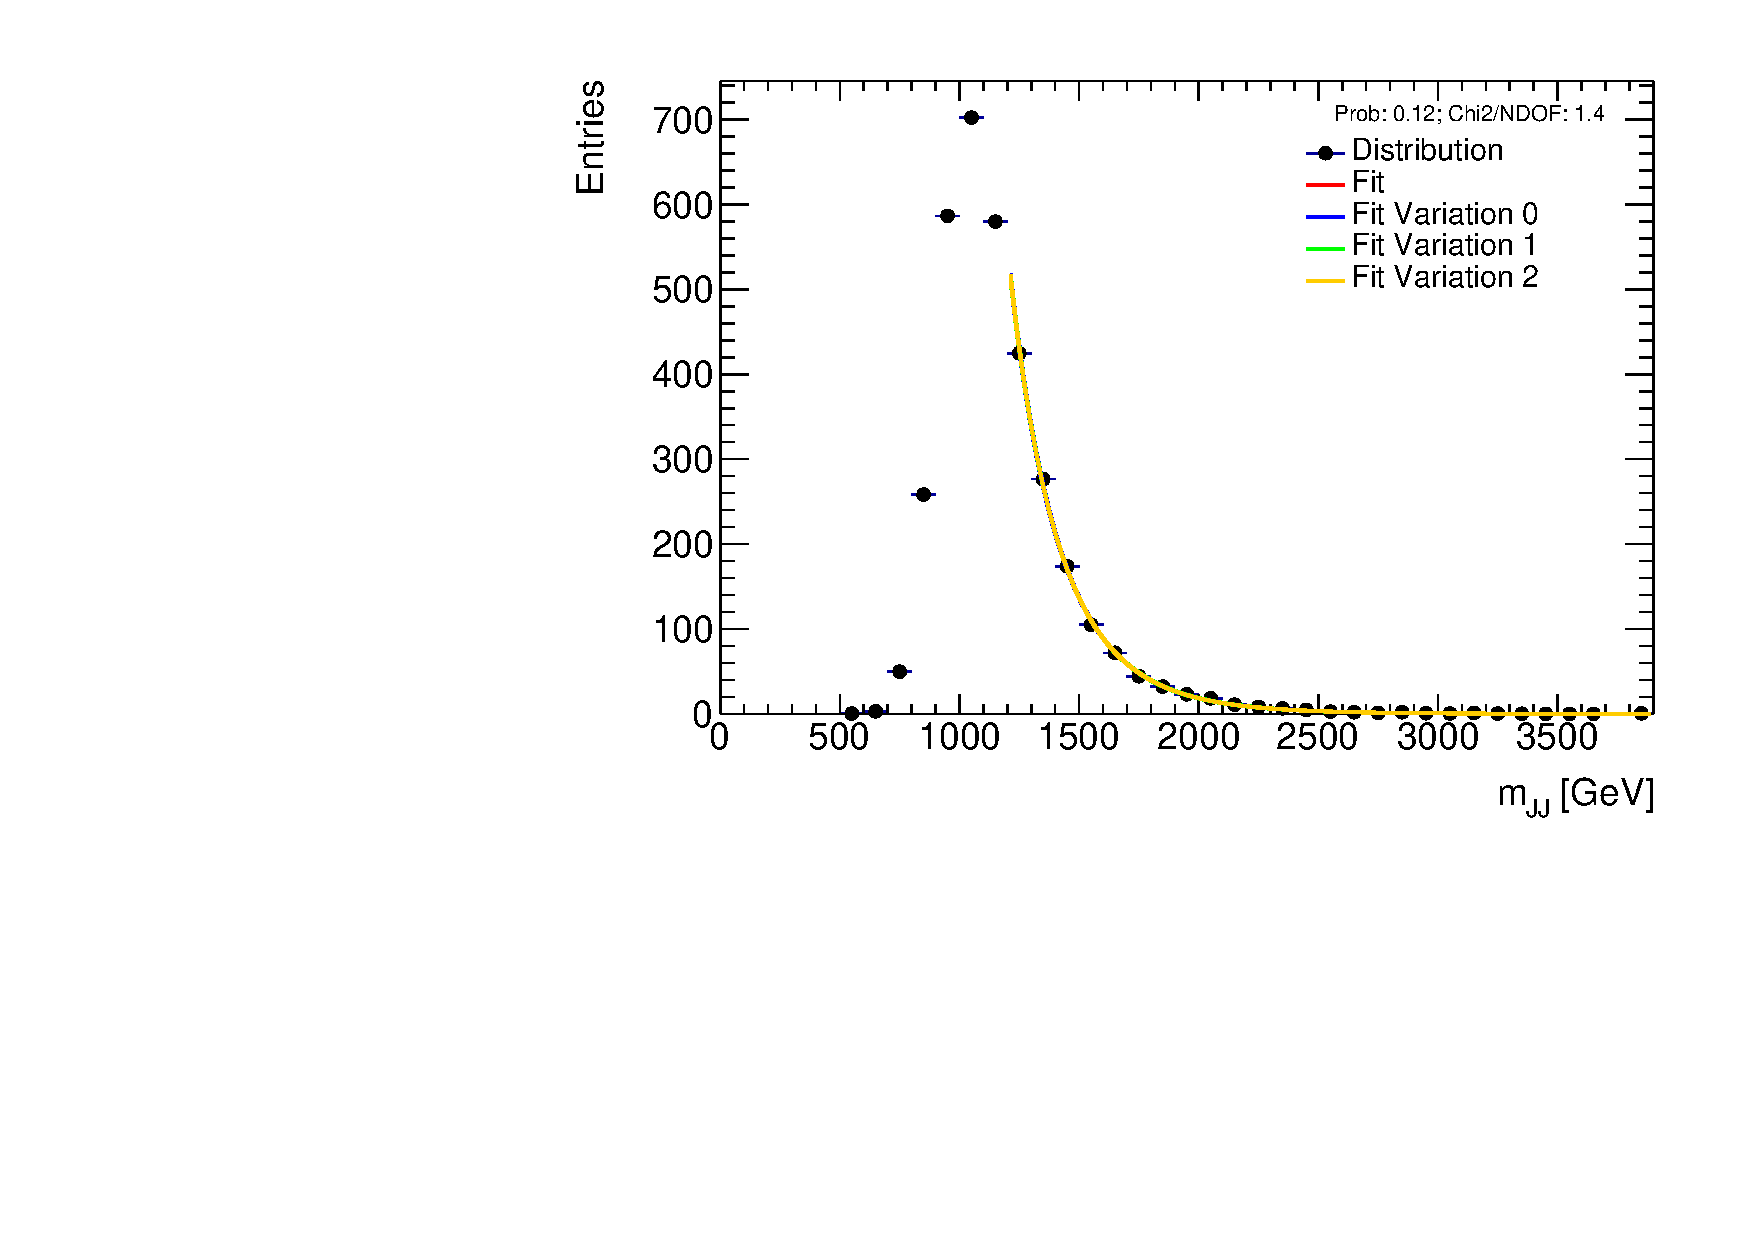
\includegraphics[width=0.45\textwidth,angle=-90]{figures/boosted/Smooth/qcd_est_TwoTag_split_Signal_mHH_pole.pdf}
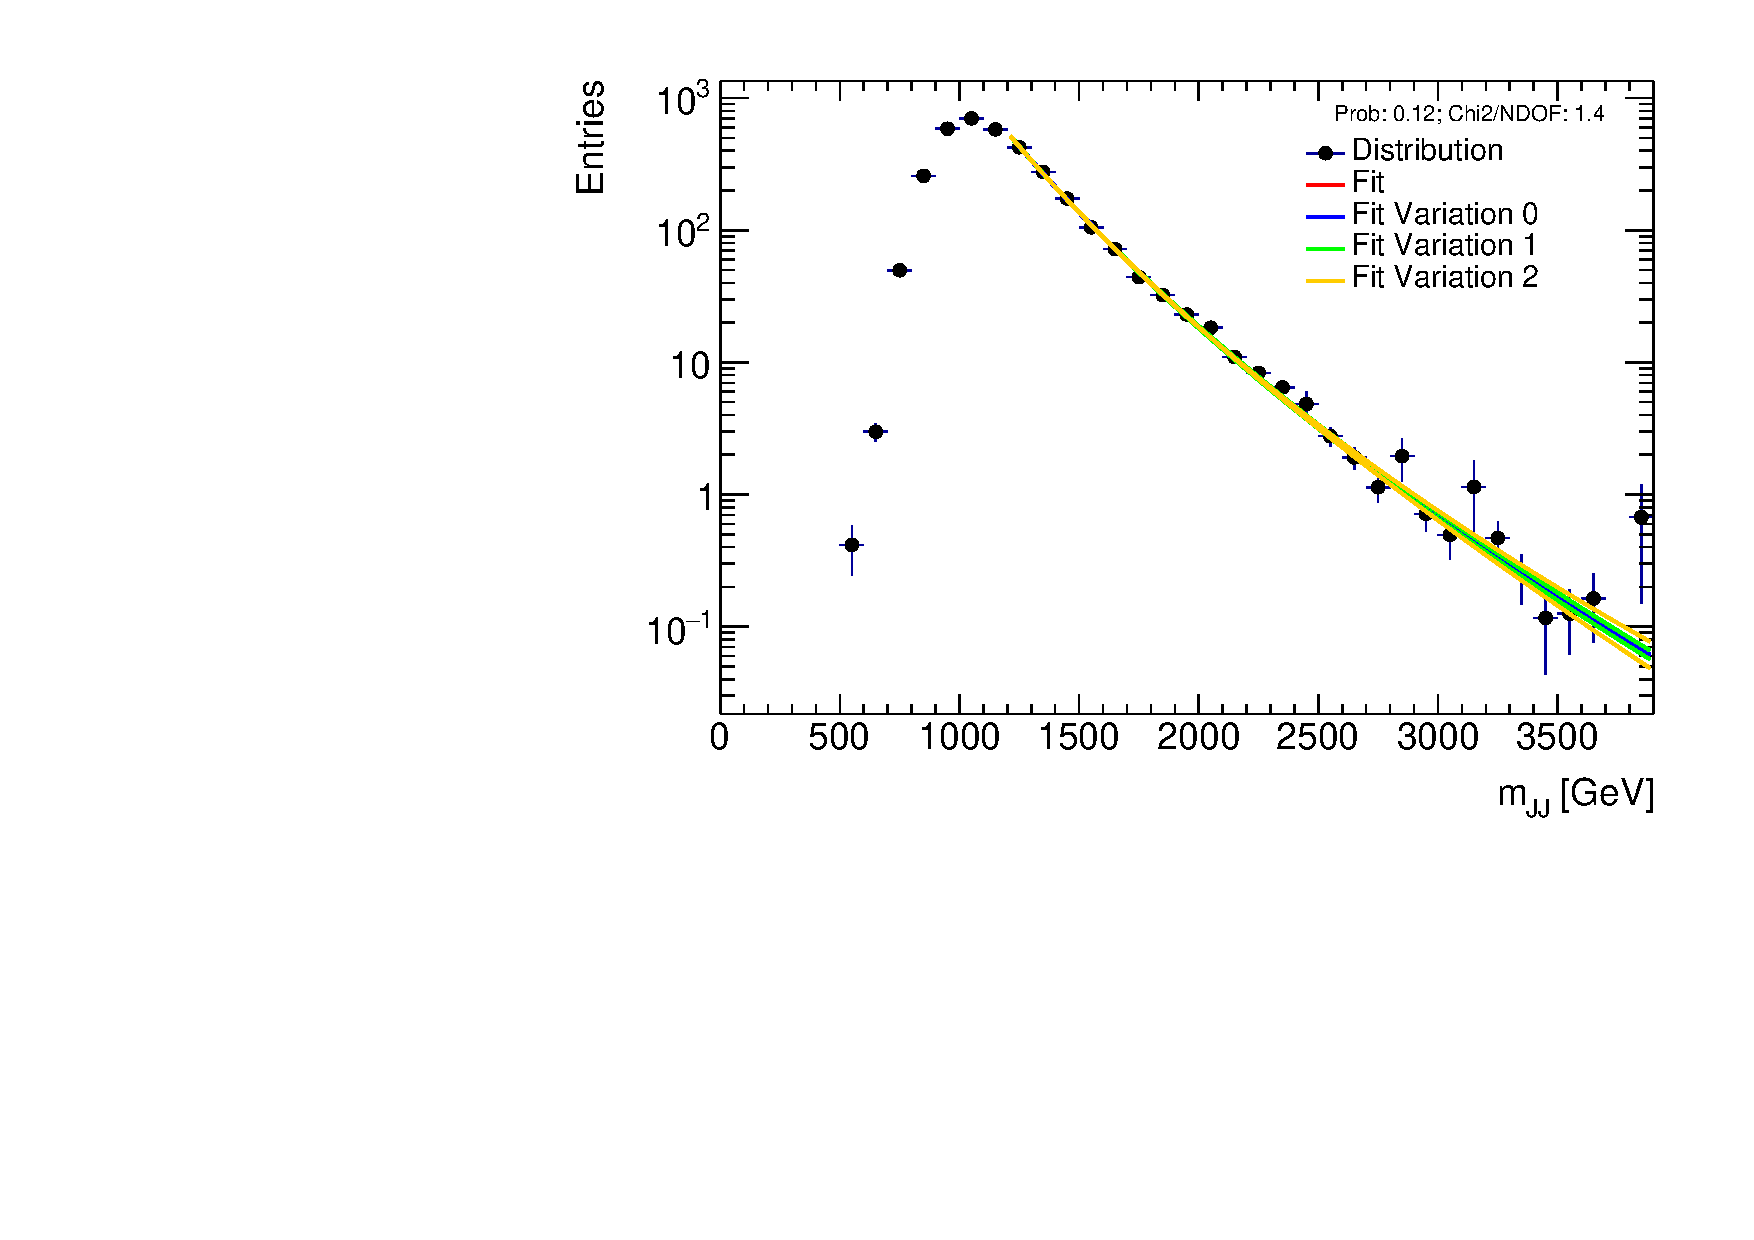
\includegraphics[width=0.45\textwidth,angle=-90]{figures/boosted/Smooth/qcd_est_TwoTag_split_Signal_mHH_pole_l.pdf}\\
%   
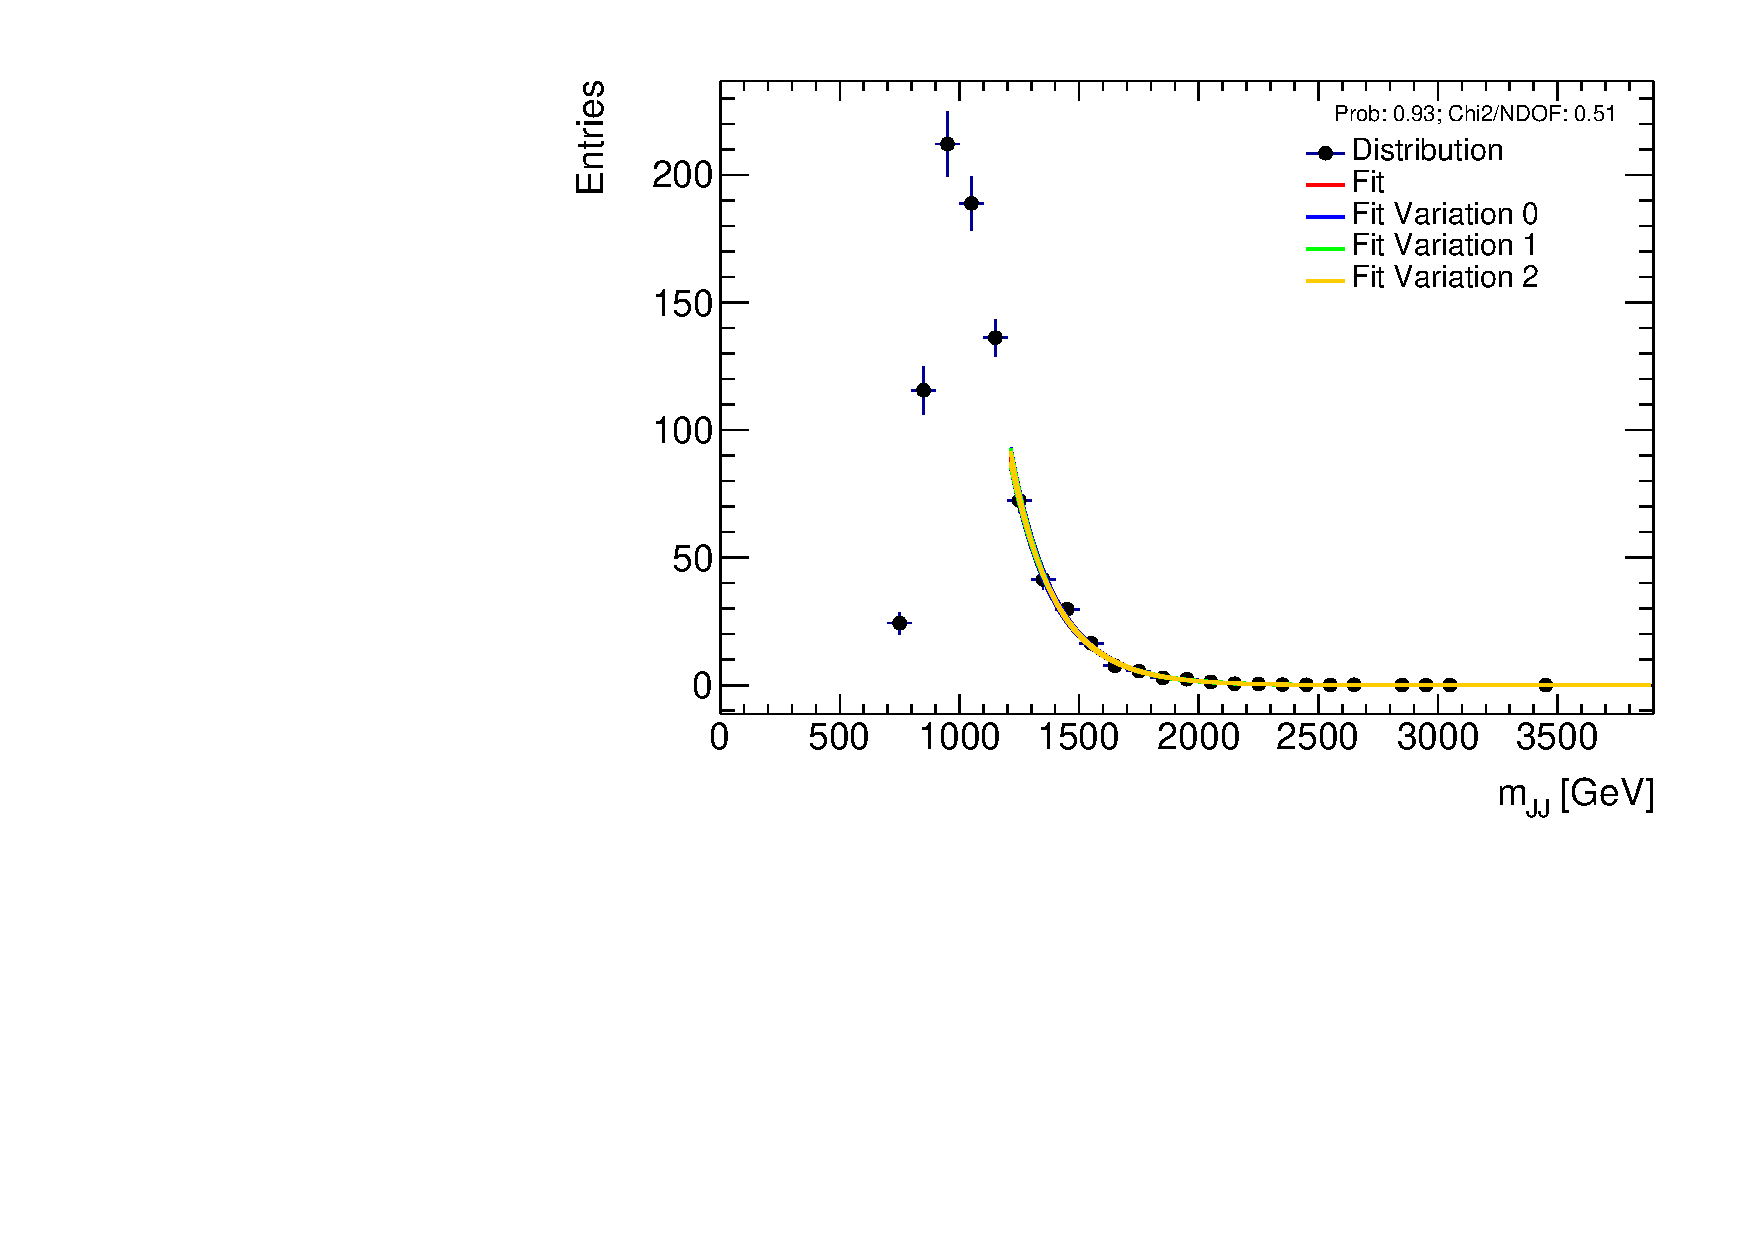
\includegraphics[width=0.45\textwidth,angle=-90]{figures/boosted/Smooth/ttbar_est_TwoTag_split_Signal_mHH_pole.pdf}
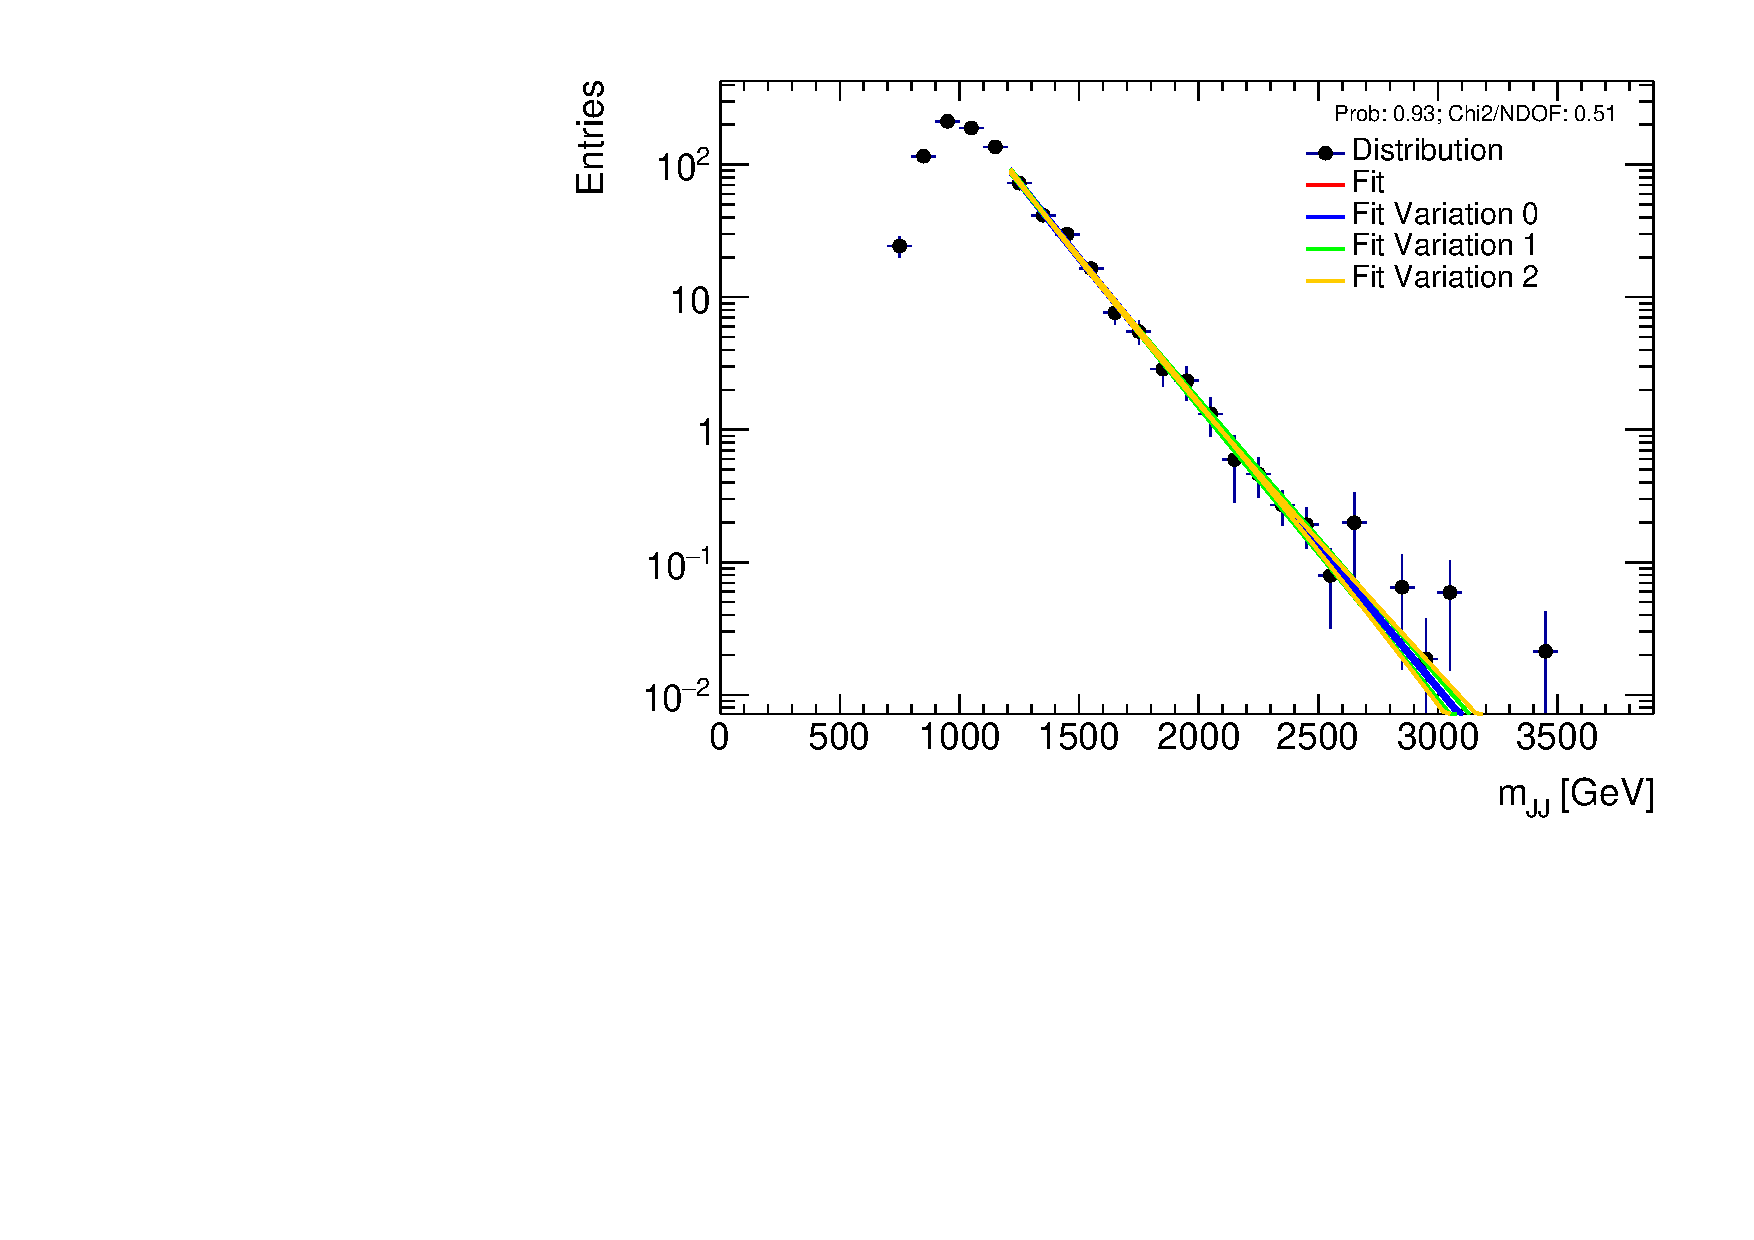
\includegraphics[width=0.45\textwidth,angle=-90]{figures/boosted/Smooth/ttbar_est_TwoTag_split_Signal_mHH_pole_l.pdf}\\
\caption{Fits for scaled background smoothing are shown for QCD (top row) and $t\bar{t}$ (bottom row) in the $2bs$ signal region.  The left figures show the distributions with linear $y$-axis scale along with the fit central value and variations. The right figures show the  distributions with log $y$-axis scale along with the fit central value and the fit variations as determined by the varying the fit parameters within uncertainties whilst taking into account parameter correlations. }
\label{fig:signal-region-mjjscaled-2bs-smoothing}
\end{center}
\end{figure}

\begin{figure}[htbp!]
\begin{center}
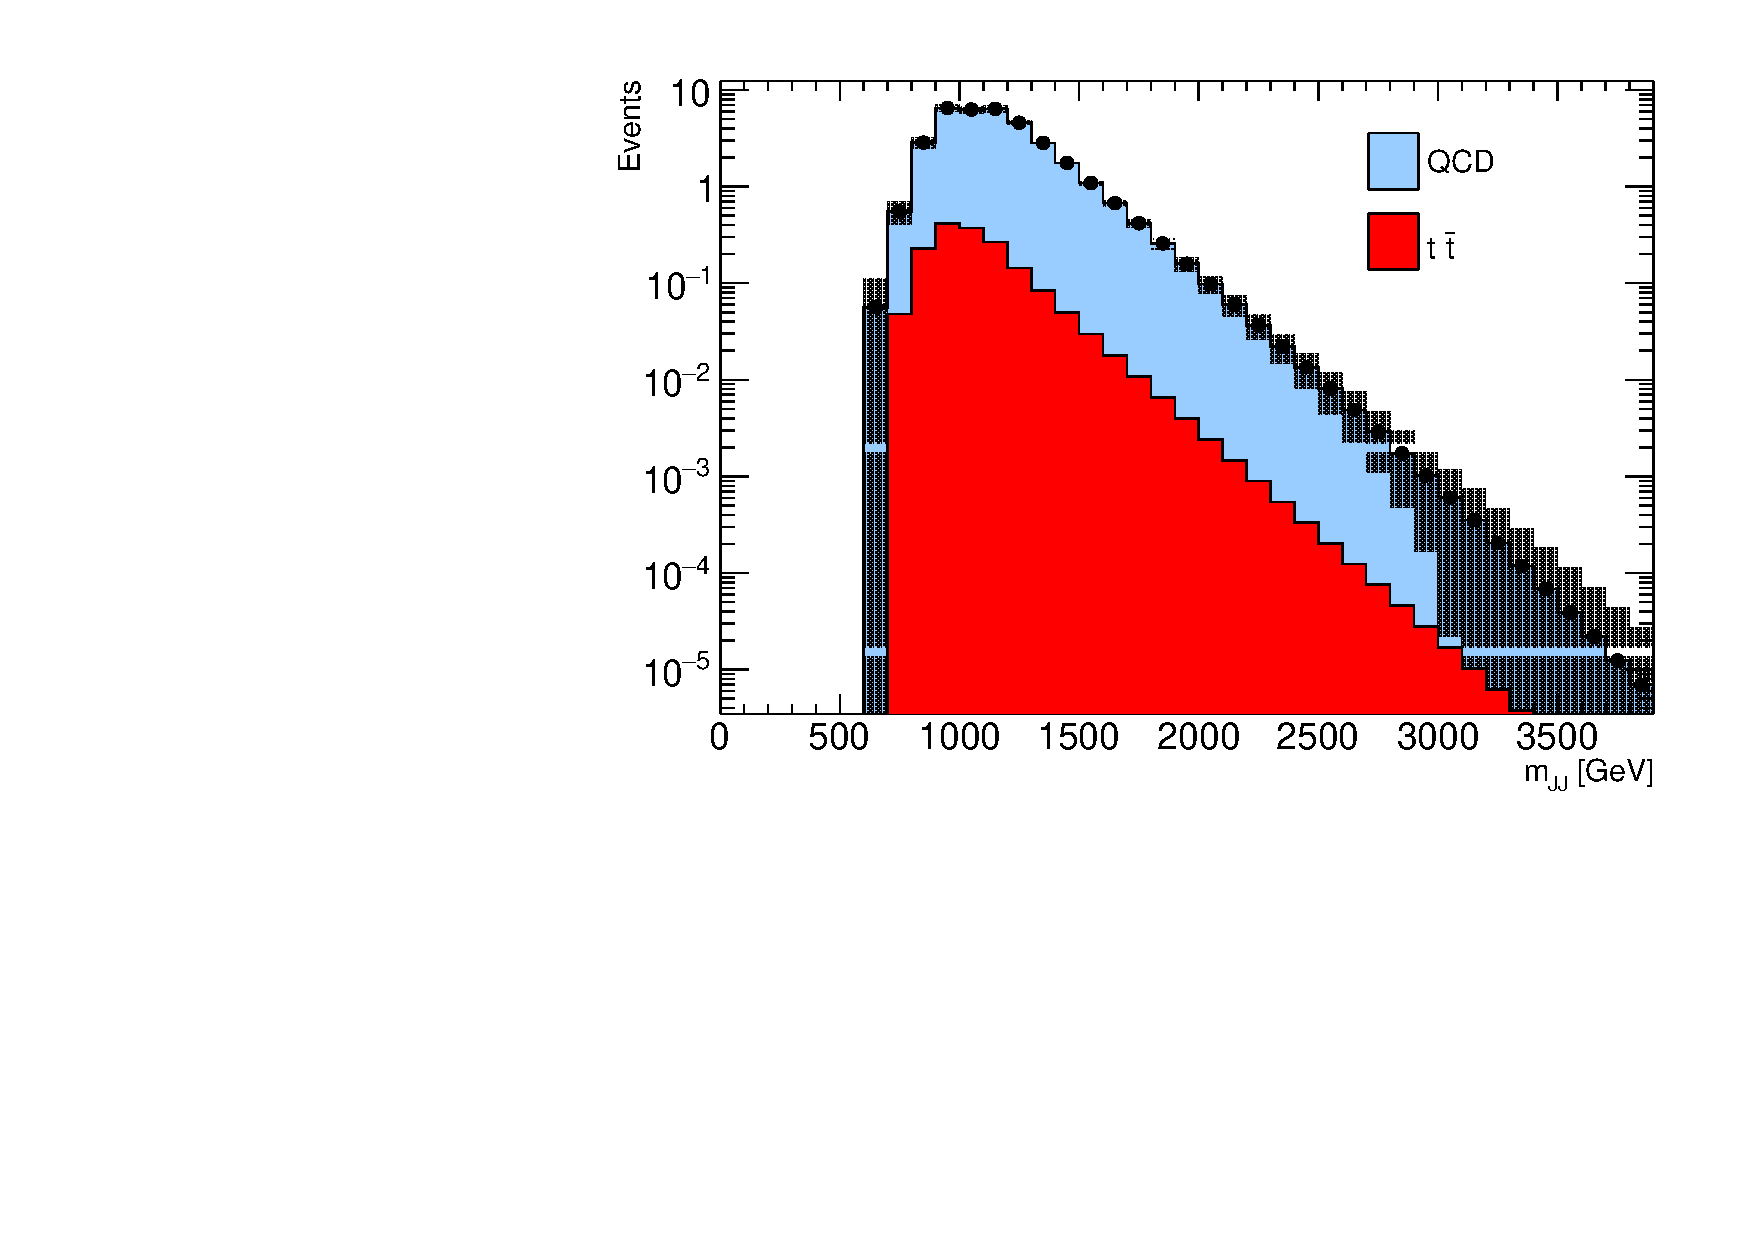
\includegraphics[width=0.45\textwidth,angle=-90]{figures/boosted/Smooth/FourTag_pole_smoothed.pdf}
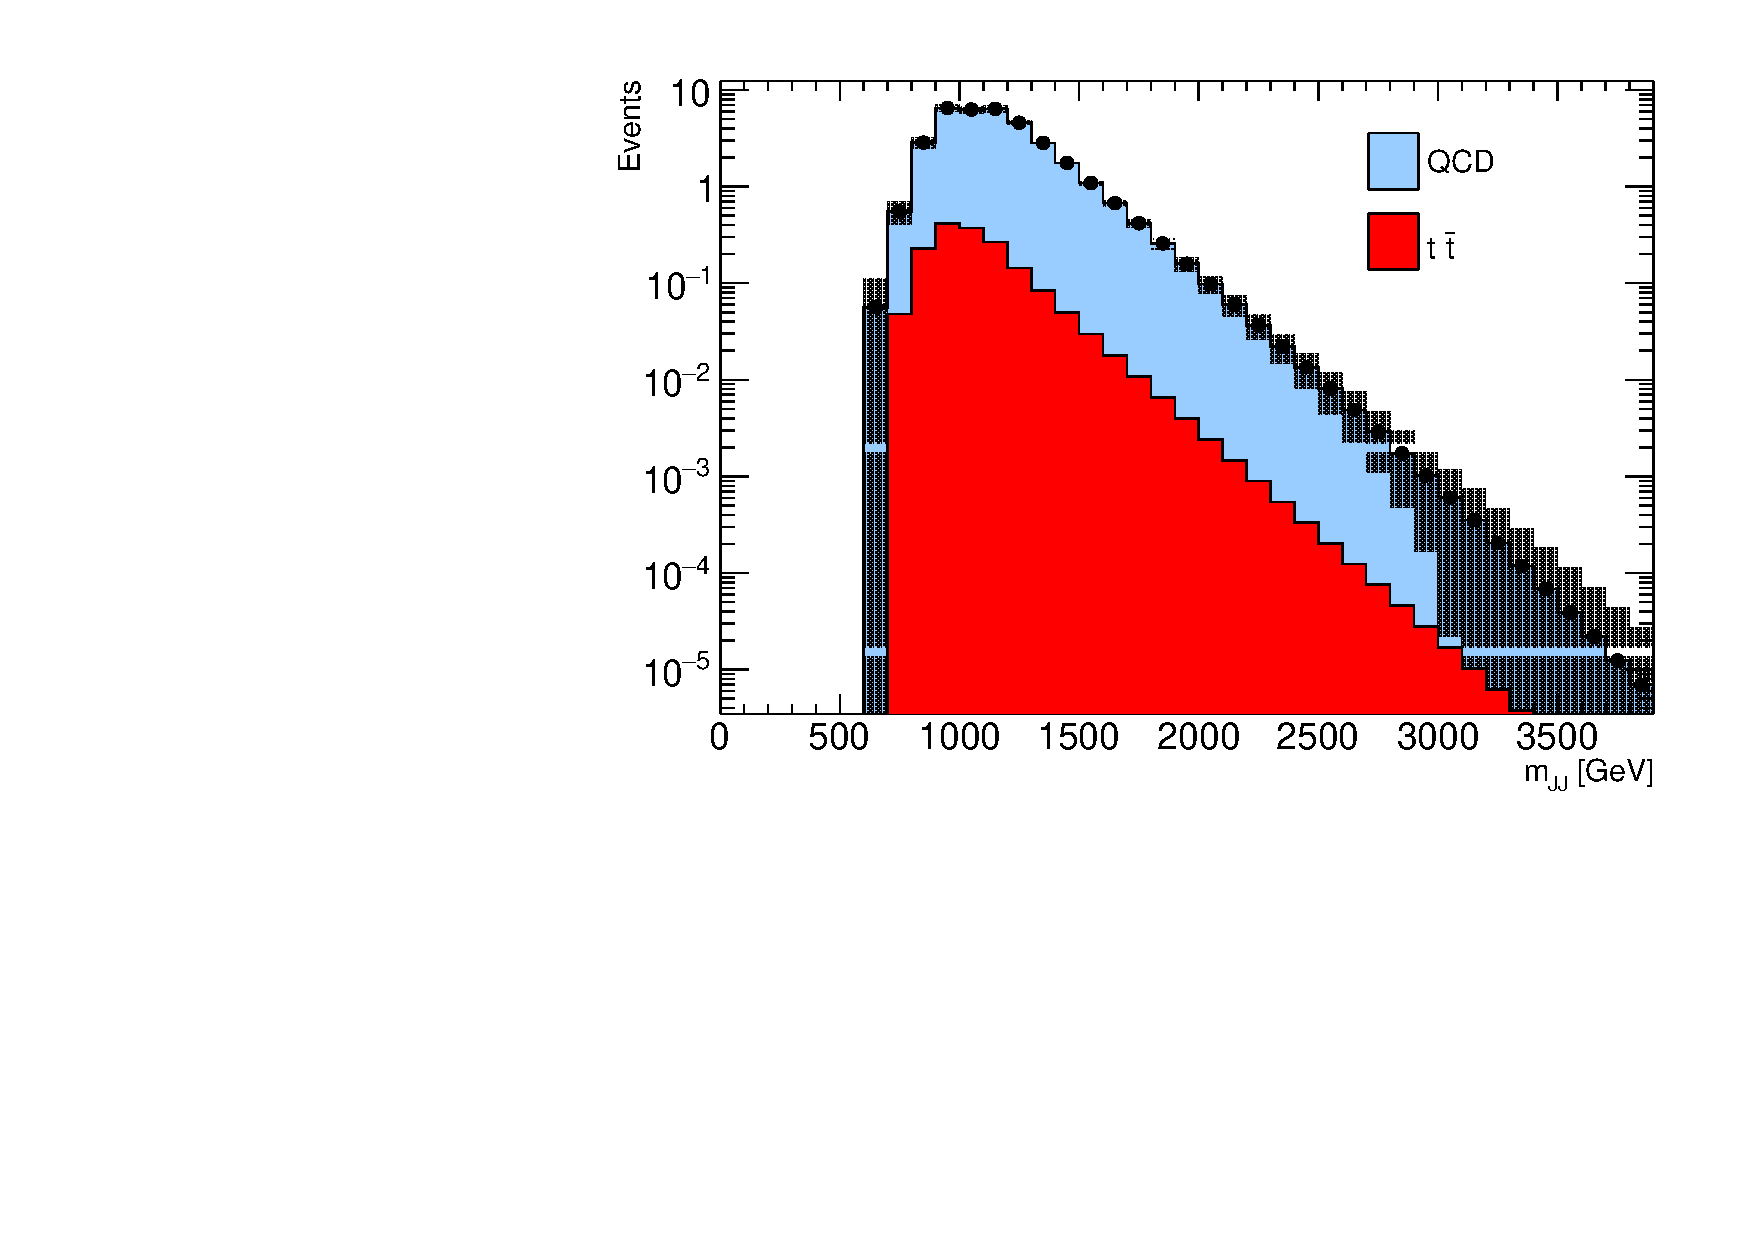
\includegraphics[width=0.45\textwidth,angle=-90]{figures/boosted/Smooth/FourTag_pole_smoothed.pdf}\\
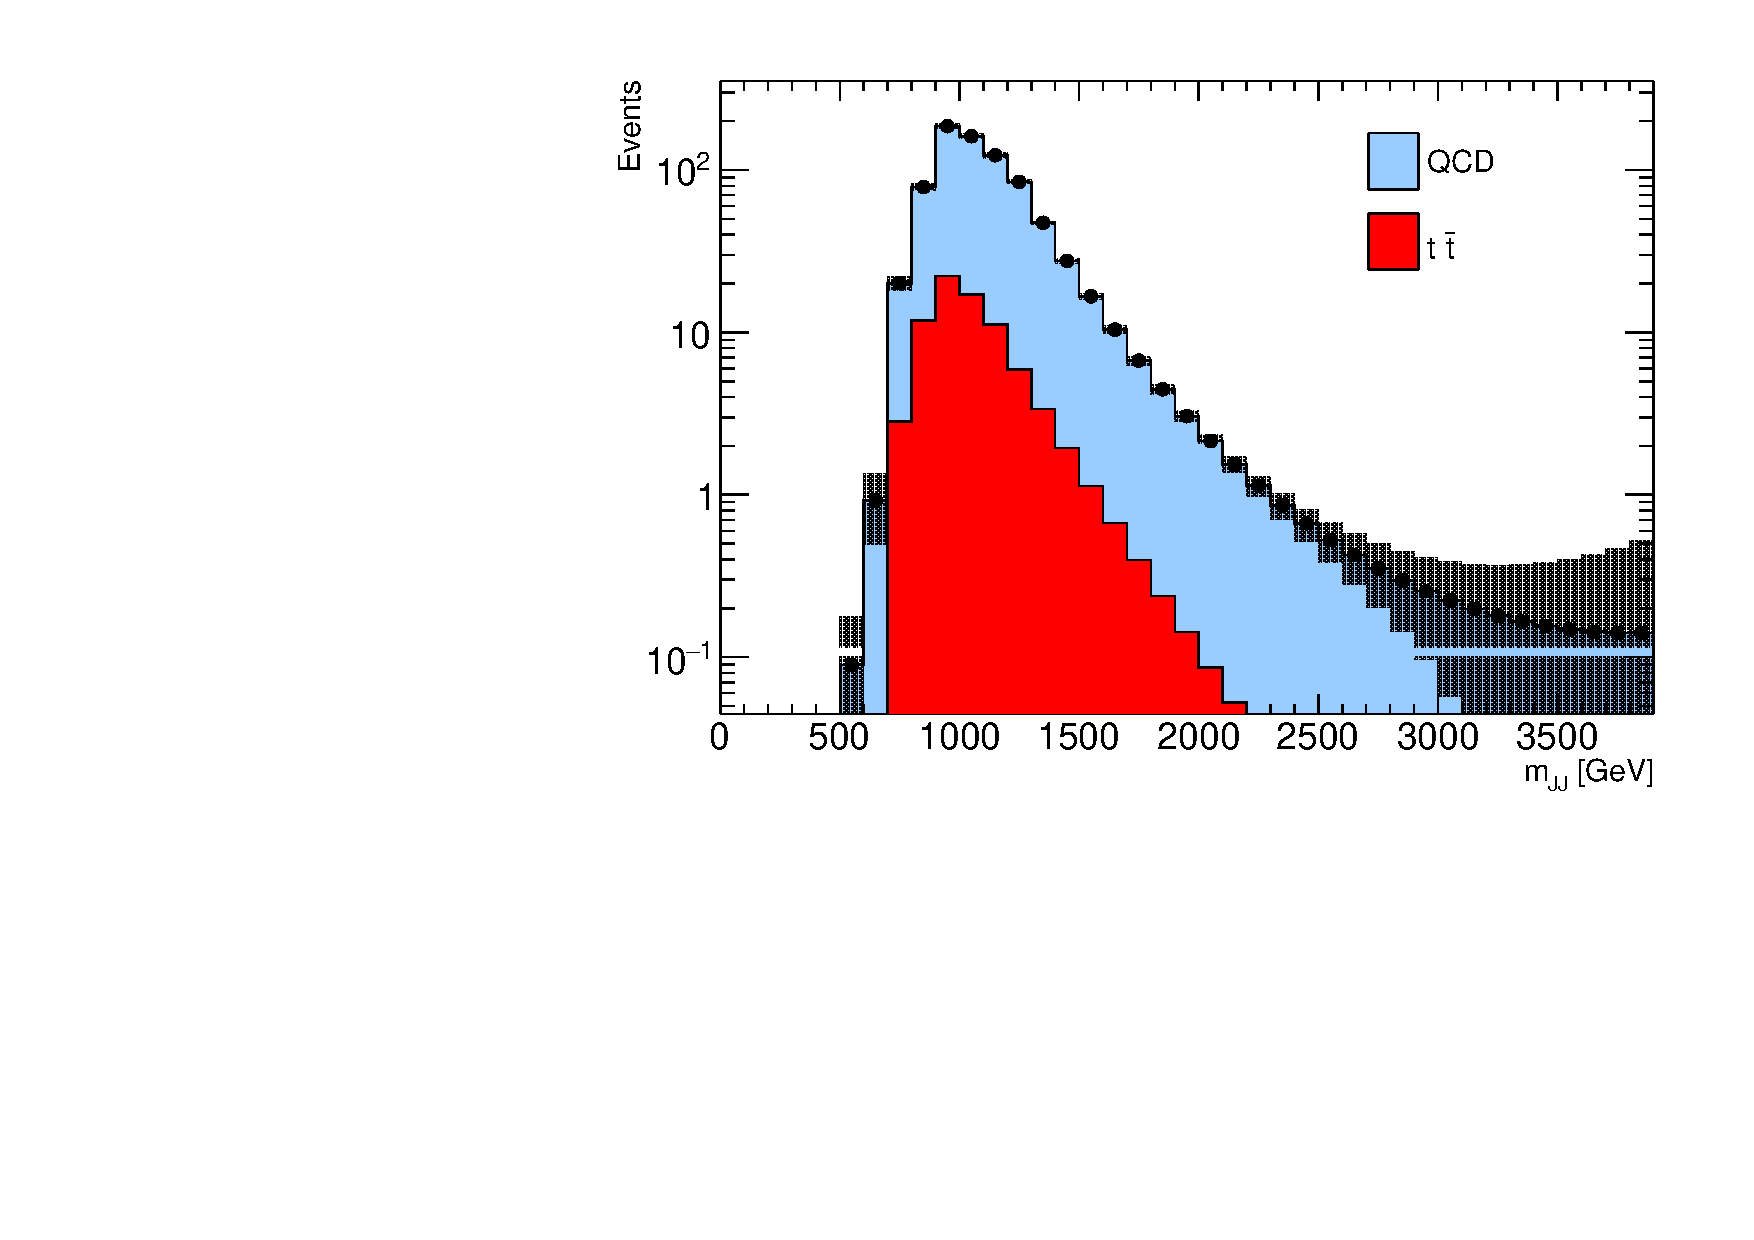
\includegraphics[width=0.45\textwidth,angle=-90]{figures/boosted/Smooth/ThreeTag_l_smoothed.pdf}
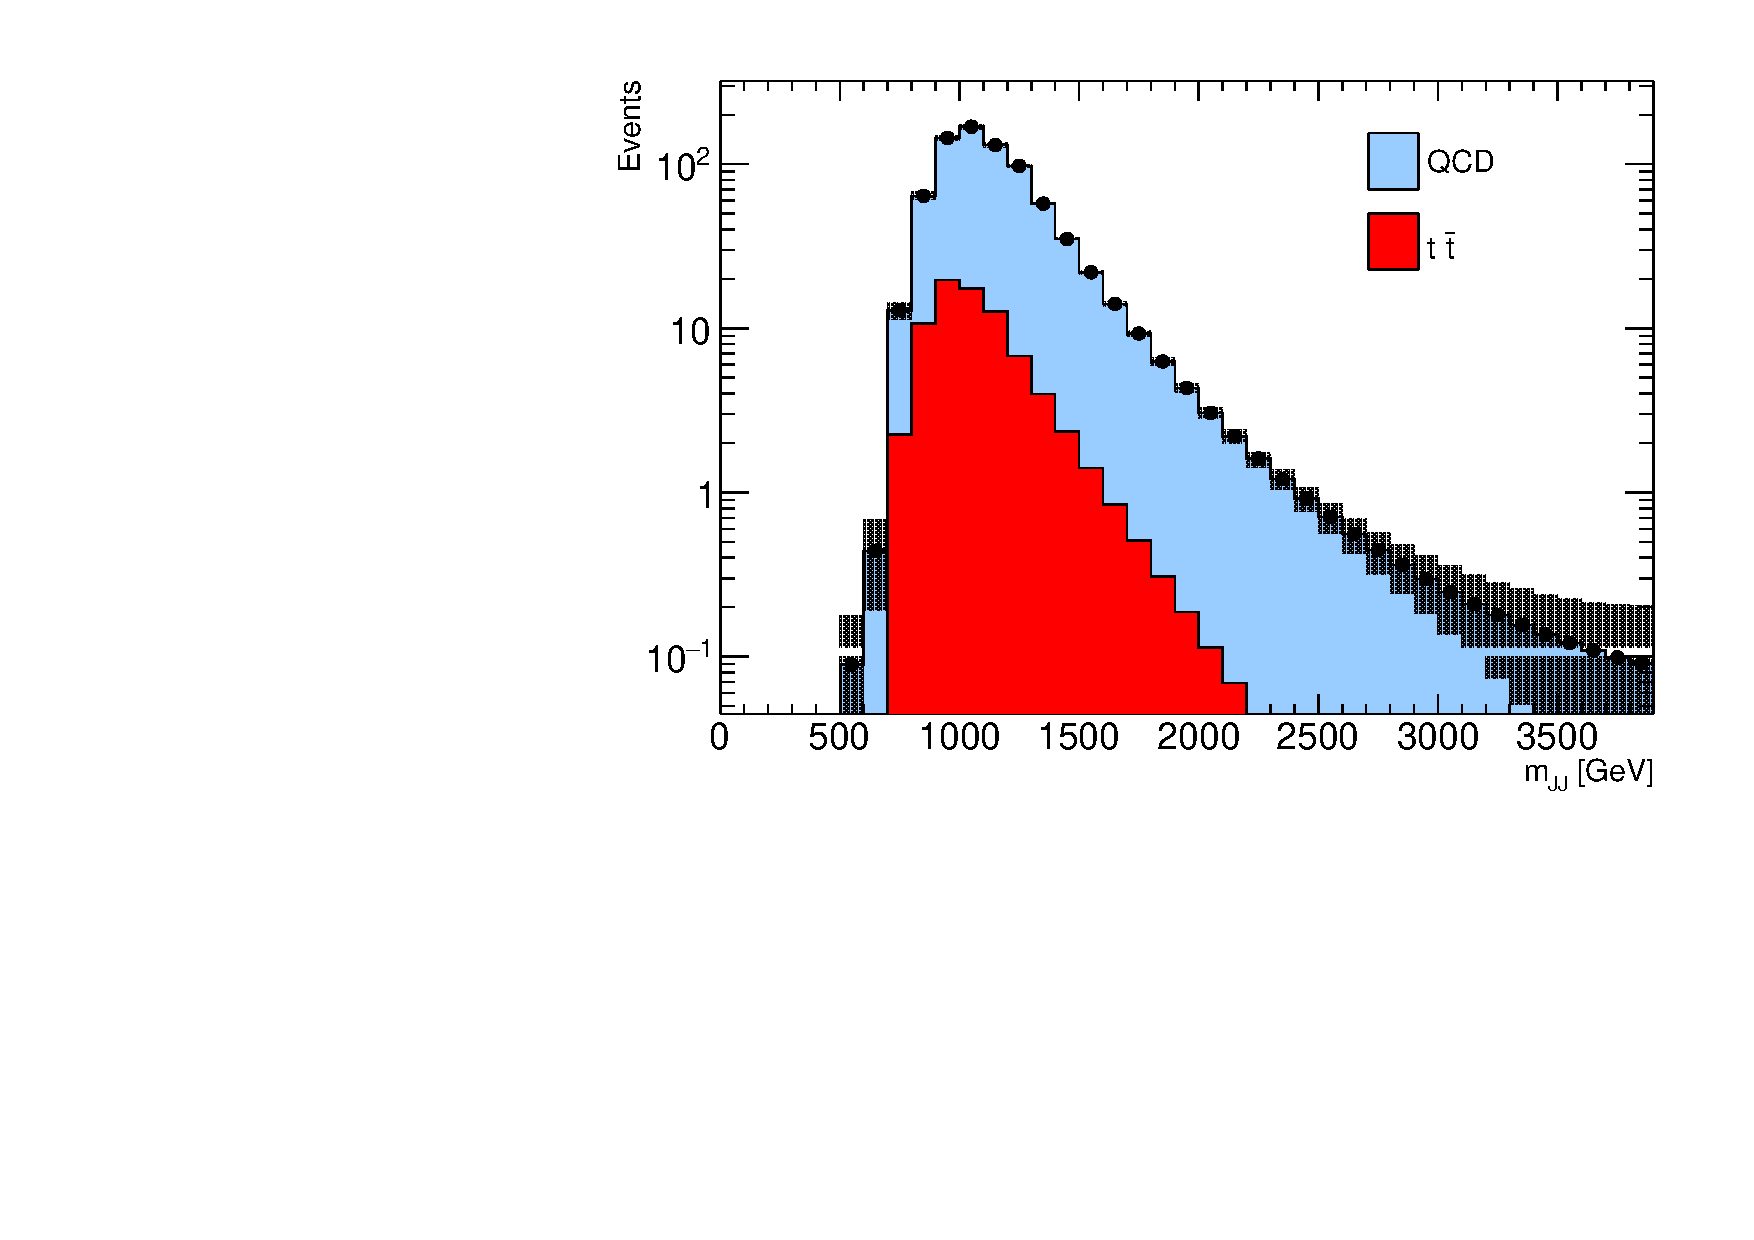
\includegraphics[width=0.45\textwidth,angle=-90]{figures/boosted/Smooth/ThreeTag_pole_smoothed.pdf}\\
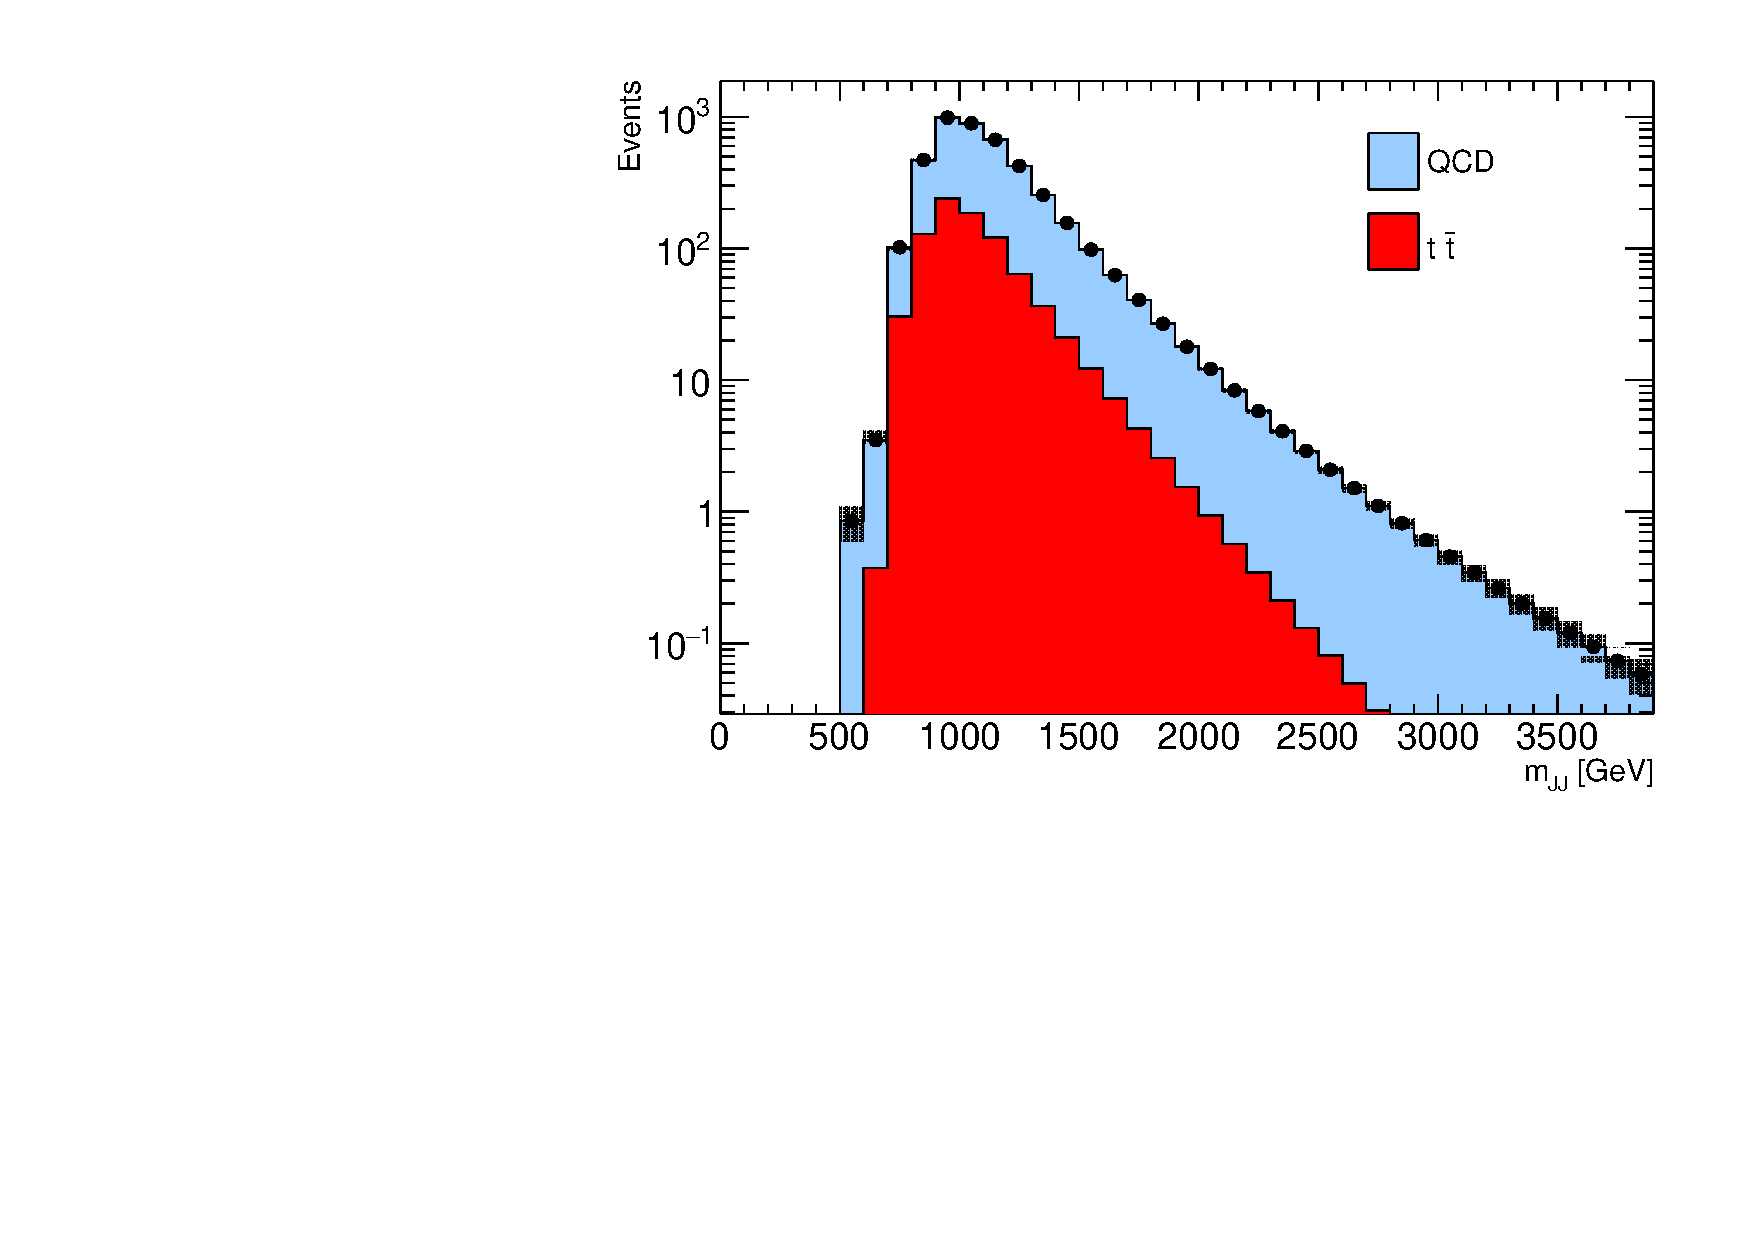
\includegraphics[width=0.45\textwidth,angle=-90]{figures/boosted/Smooth/TwoTag_split_l_smoothed.pdf}
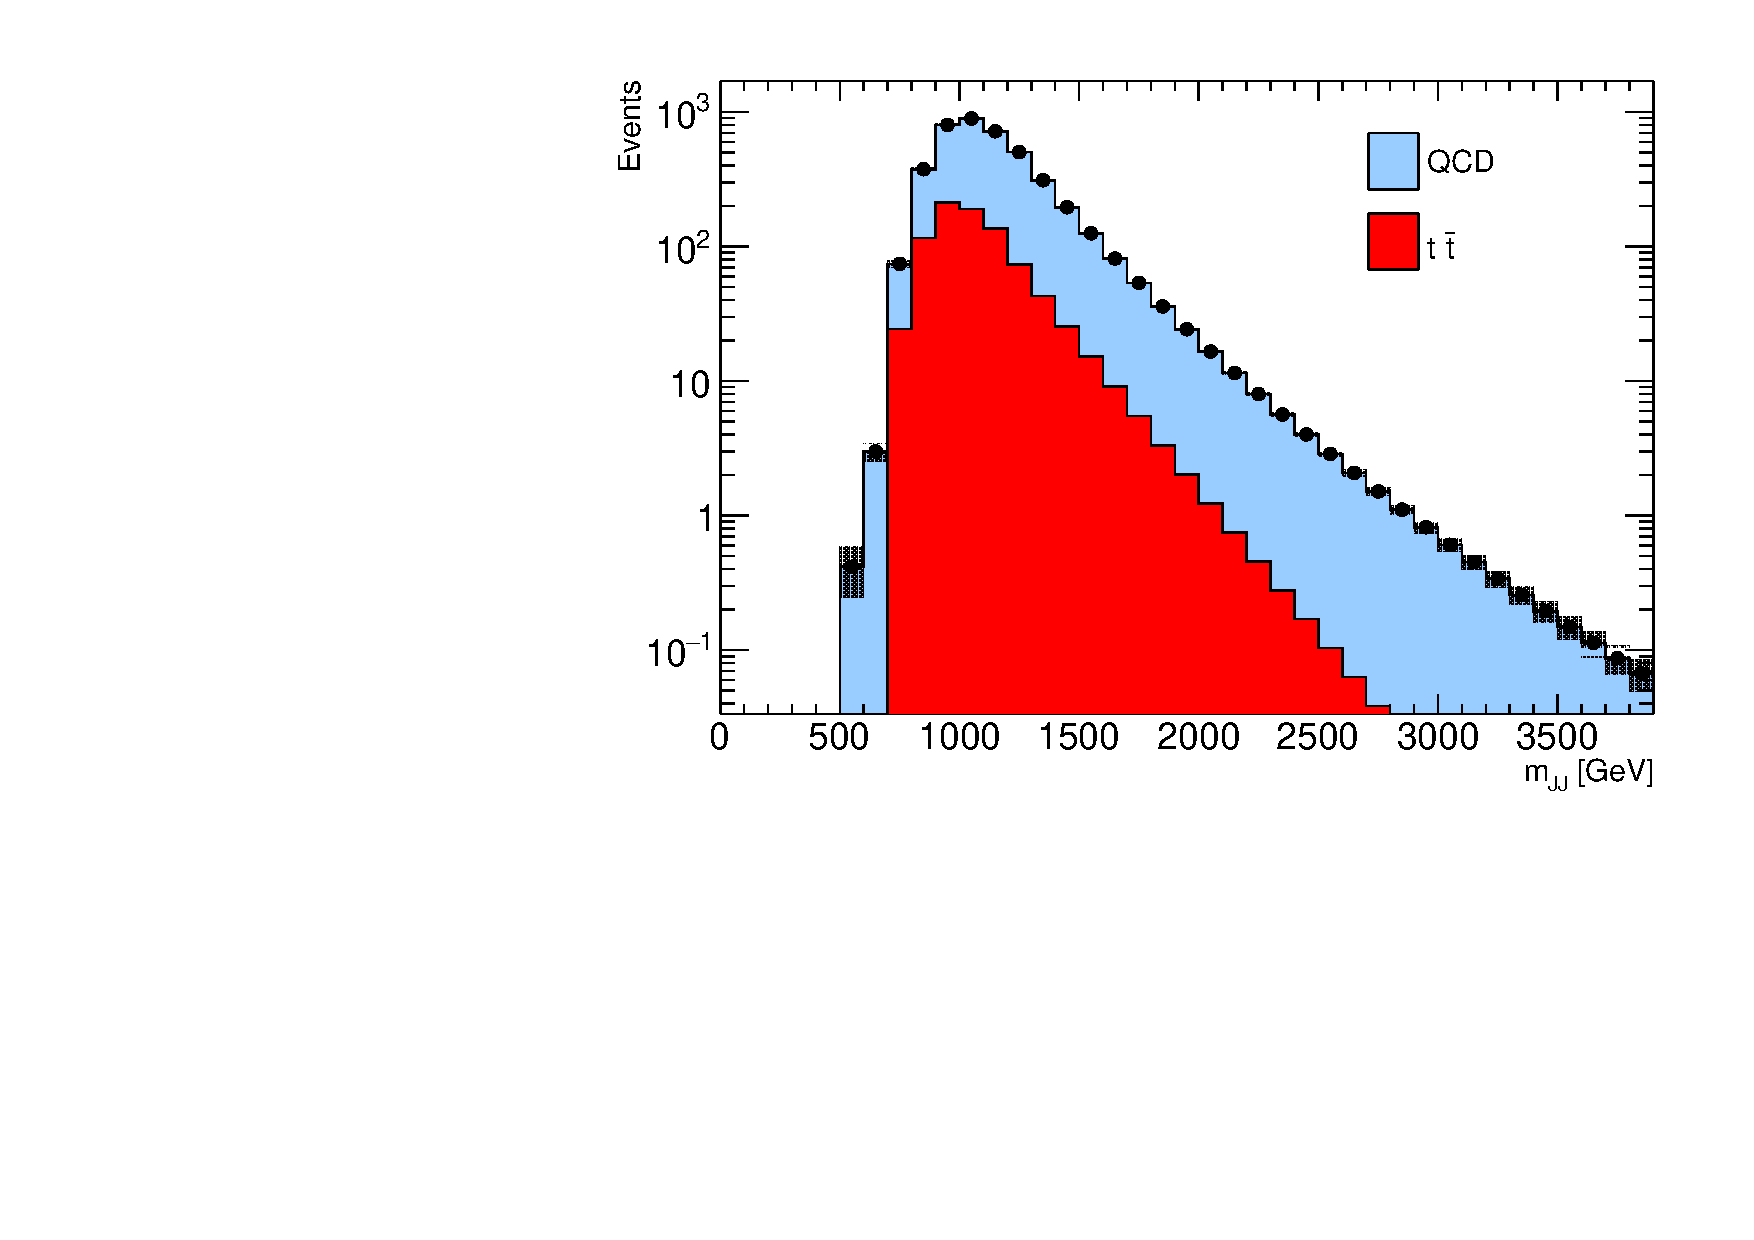
\includegraphics[width=0.45\textwidth,angle=-90]{figures/boosted/Smooth/TwoTag_split_pole_smoothed.pdf}\\
\caption{Smoothed MJJ (left) and scaled MJJ (right) background estimations the $4b$ (top), $3b$ (middle), and $2bs$ (bottom) signal regions. Smoothing statistical and systematic uncertainties from smoothing parameter variations are shown here. }
\label{fig:fig:signal-region-mjjscaled-smooth-bkg}
\end{center}
\end{figure}

\begin{figure}[htbp!]
\begin{center}
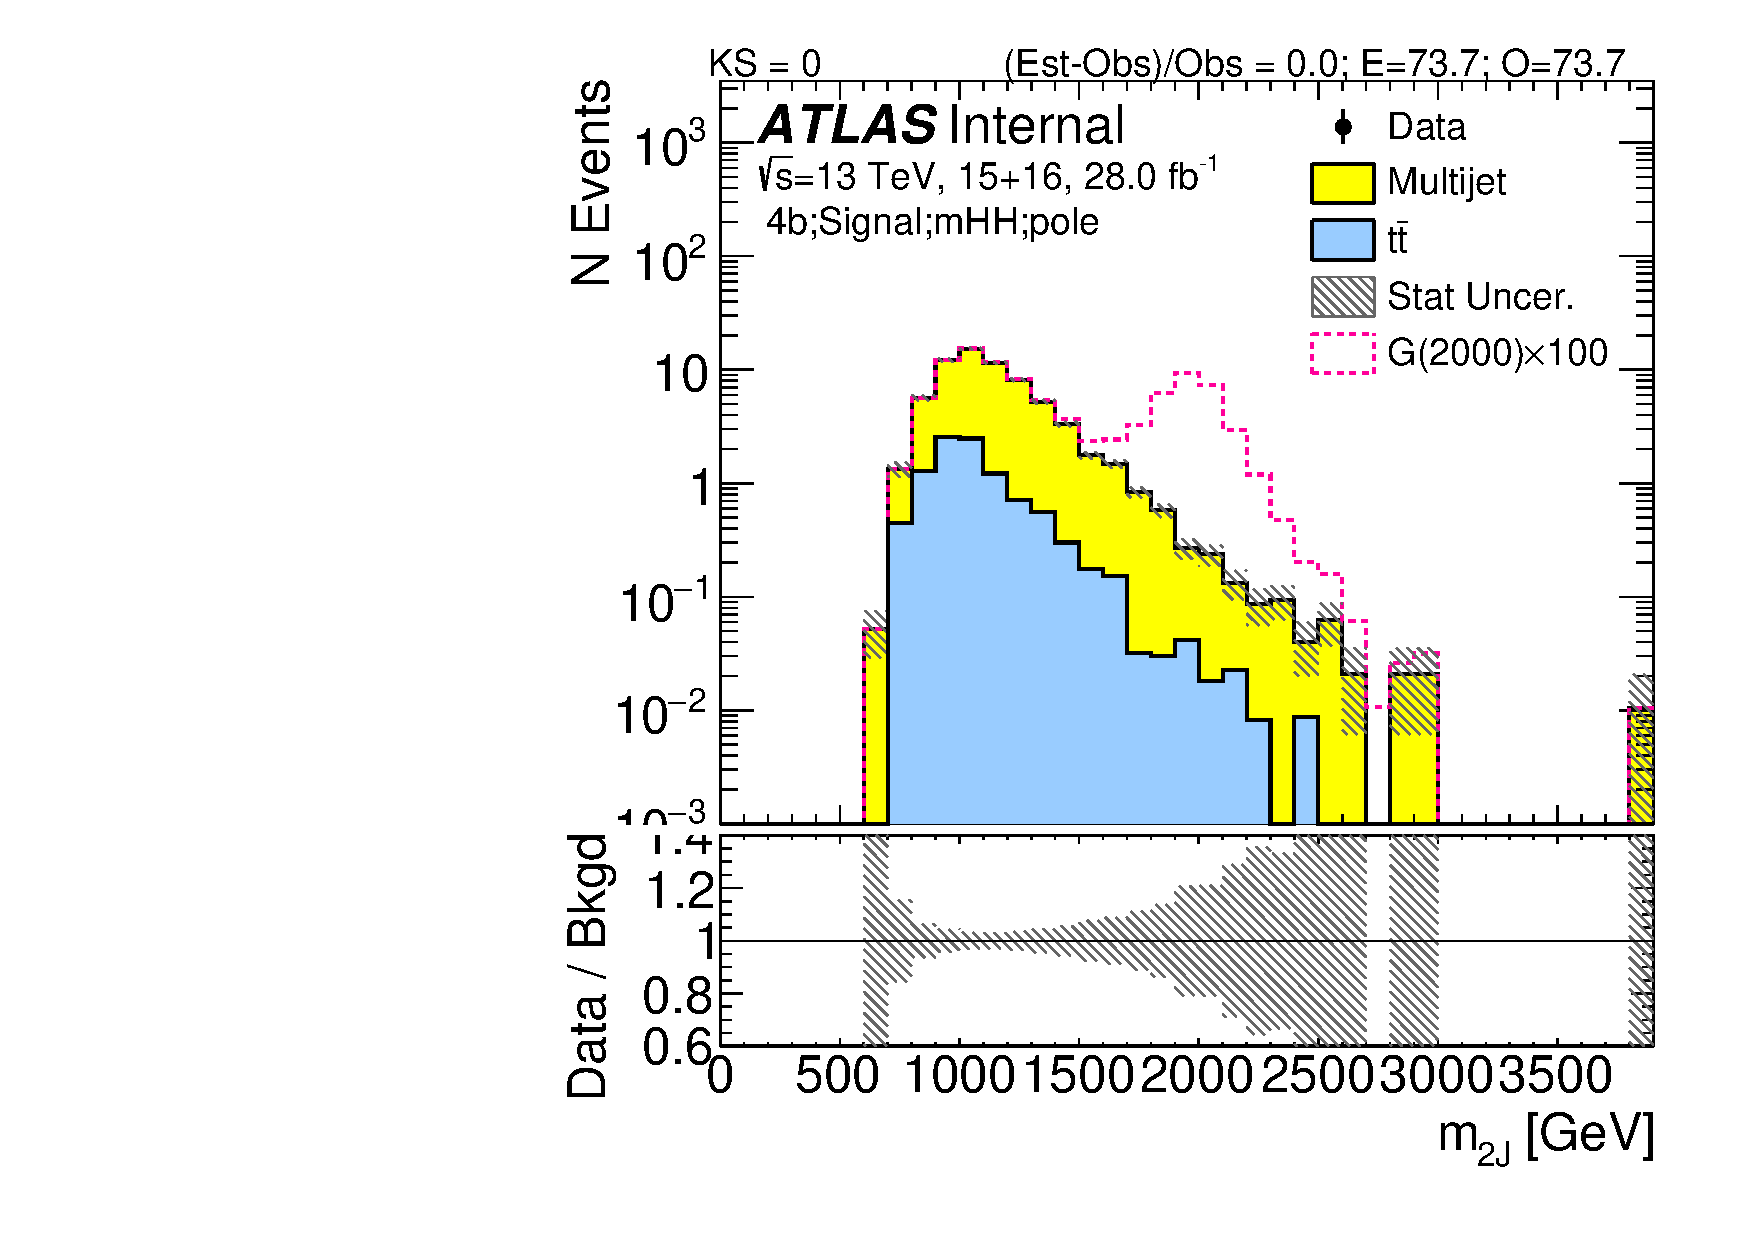
\includegraphics[width=0.45\textwidth,angle=-90]{figures/boosted/Signal/b77_FourTag_Signal_mHH_pole_1_blind.pdf}\\
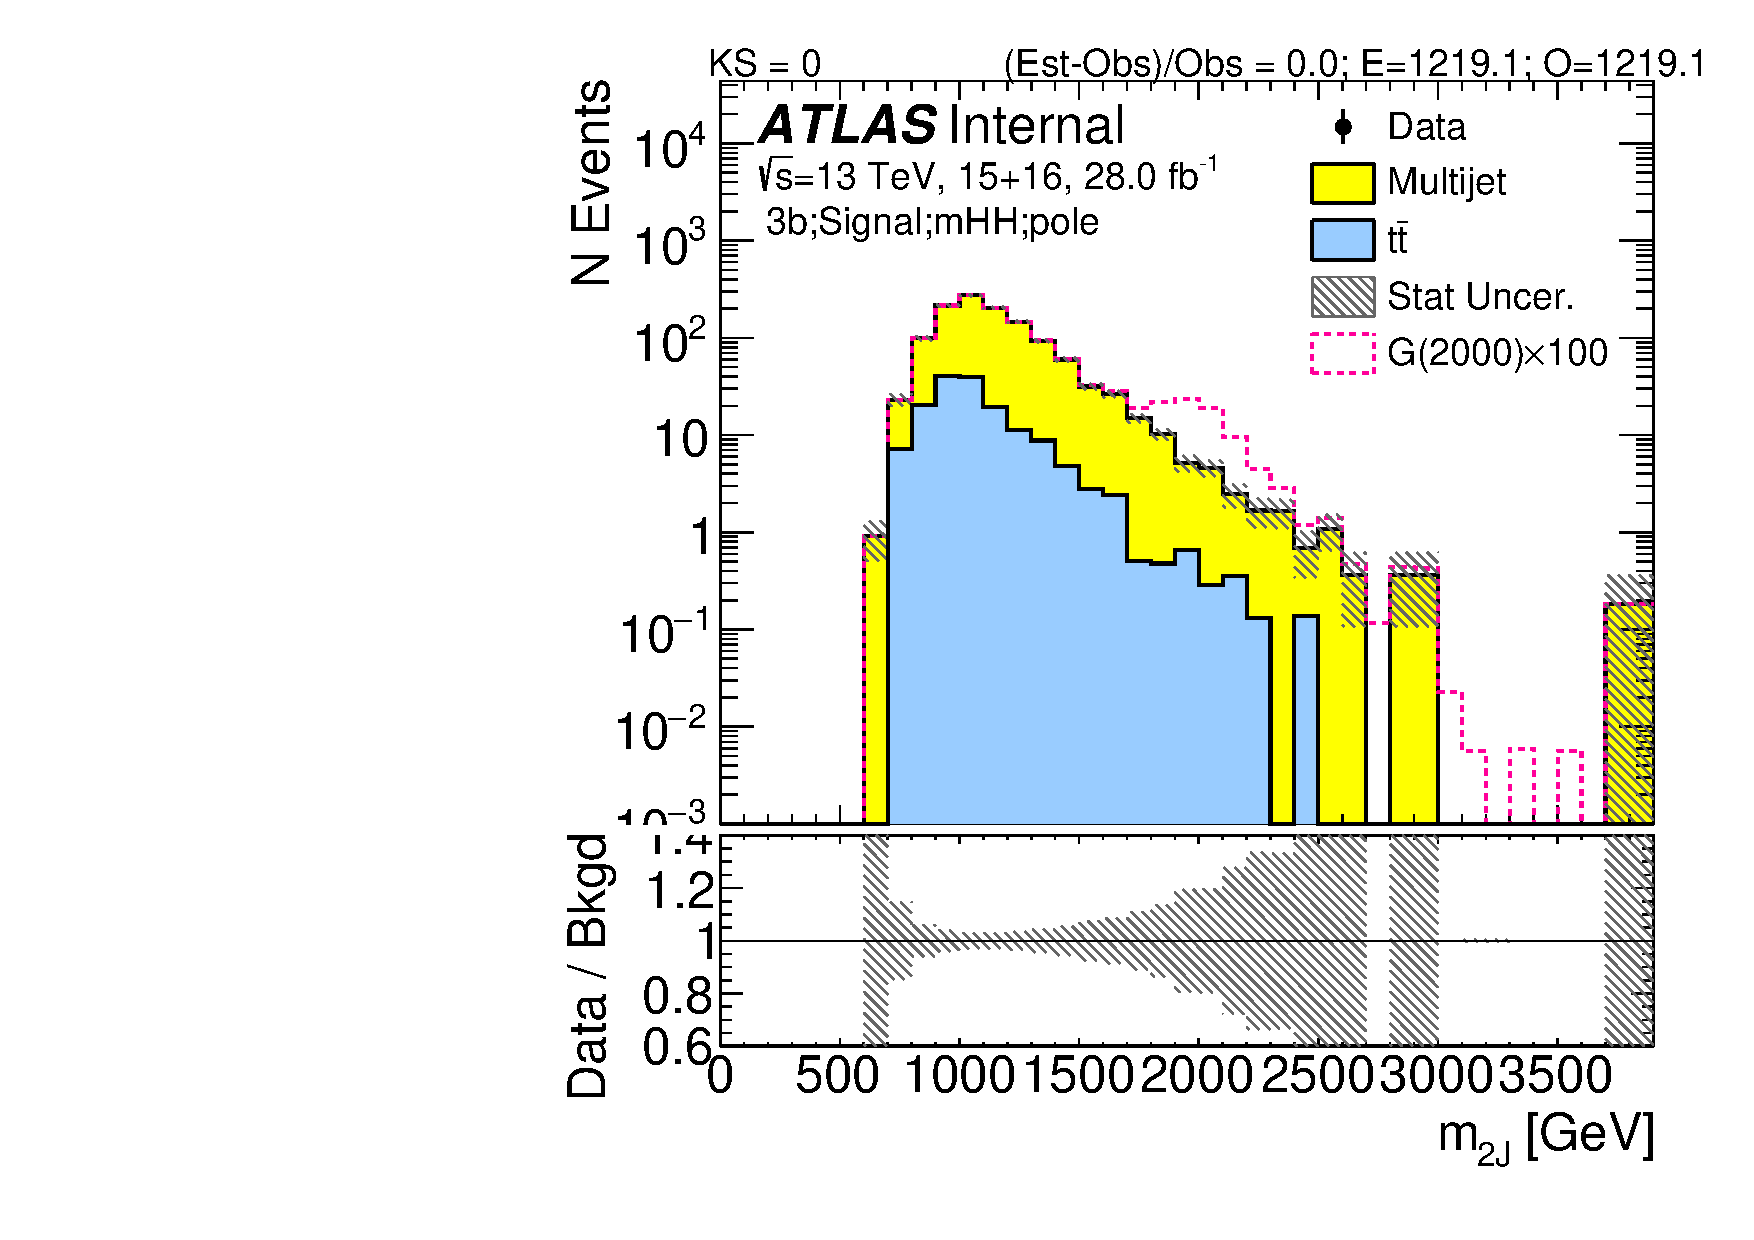
\includegraphics[width=0.45\textwidth,angle=-90]{figures/boosted/Signal/b77_ThreeTag_Signal_mHH_pole_1_blind.pdf}\\
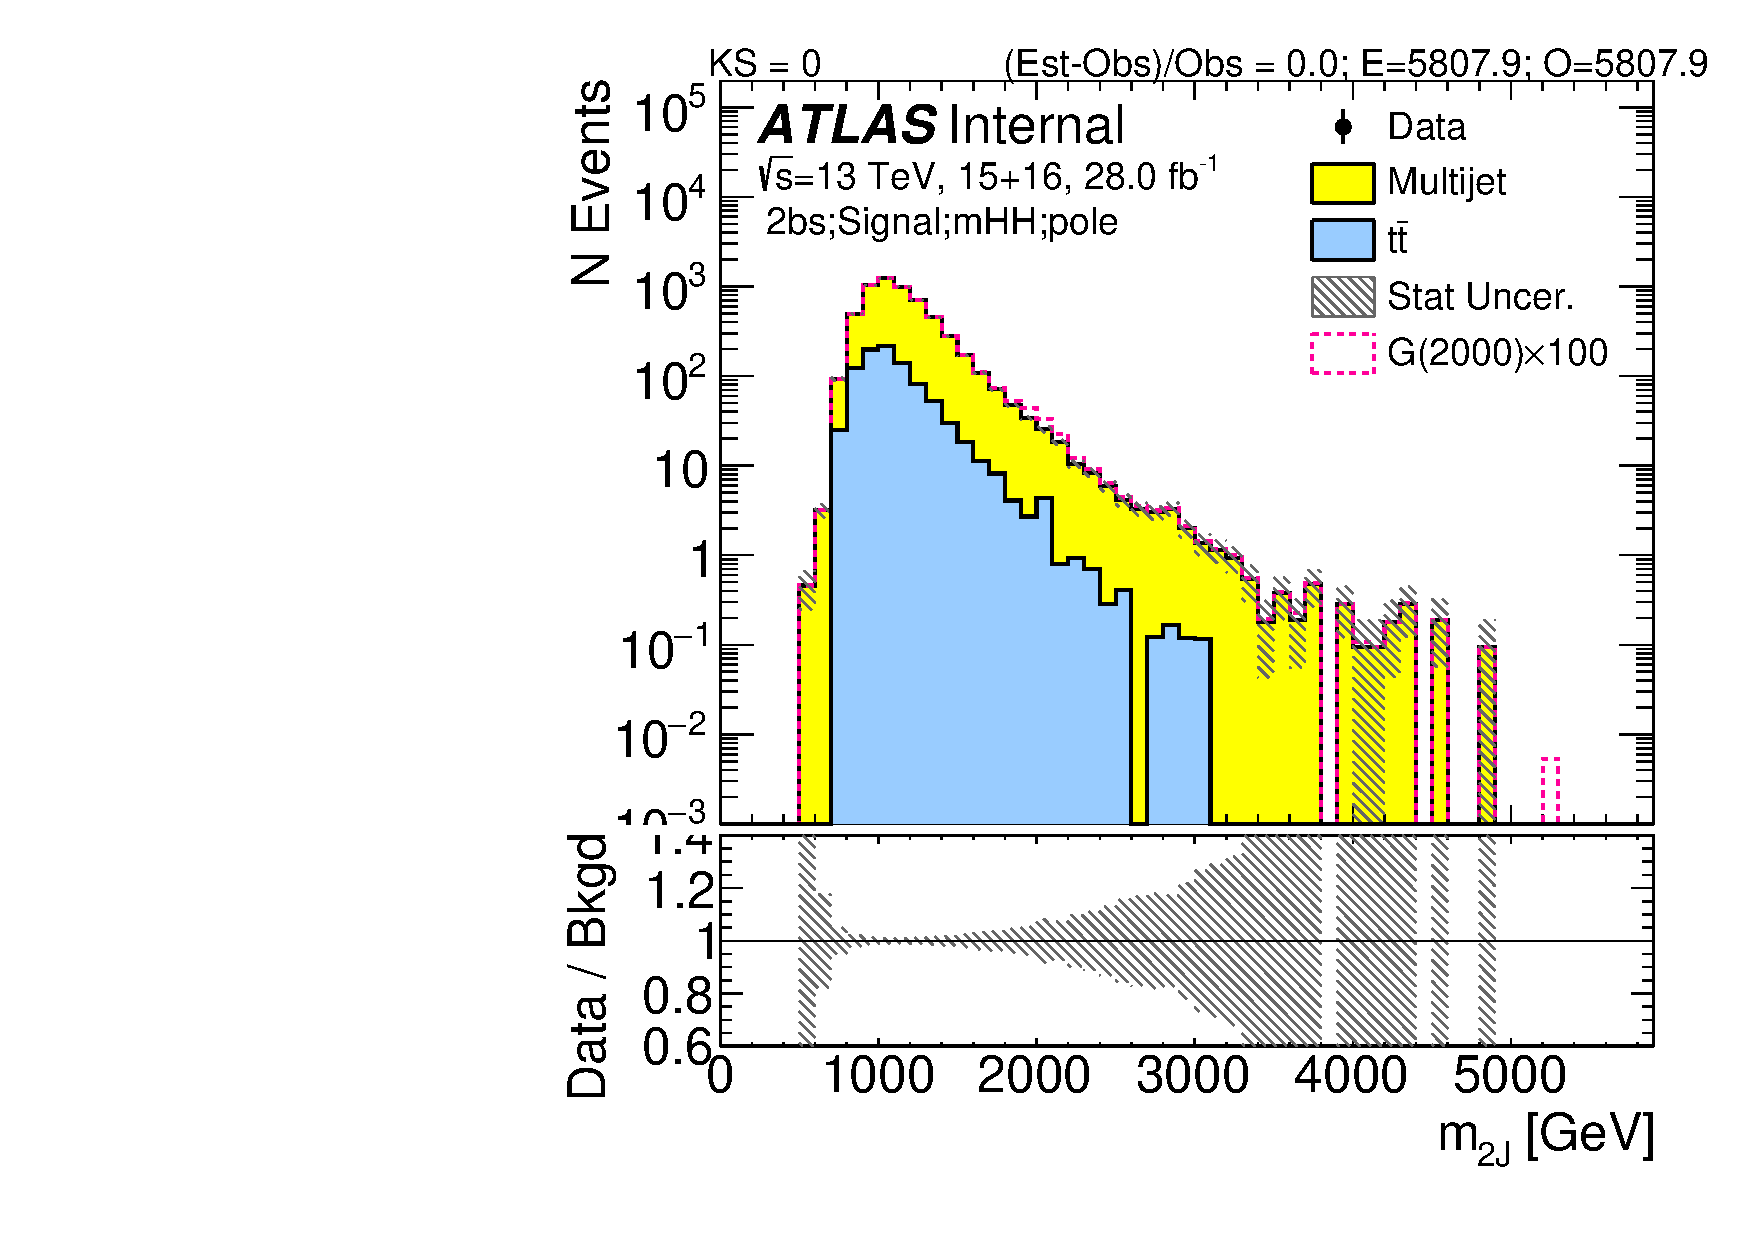
\includegraphics[width=0.45\textwidth,angle=-90]{figures/boosted/Signal/b77_TwoTag_split_Signal_mHH_pole_1_blind.pdf}
\end{center}
\caption{Background prediction for $4b$ (top), $3b$ (middle), and $2bs$ (bottom) signal region using scaled di-jet mass before smoothing. The uncertainty band includes only statistical uncertainties.}
\label{fig:signal-region-mjjscaled-nonsmooth-bkg-noSYS}
\end{figure}


\begin{figure}[htbp!]
\begin{center}
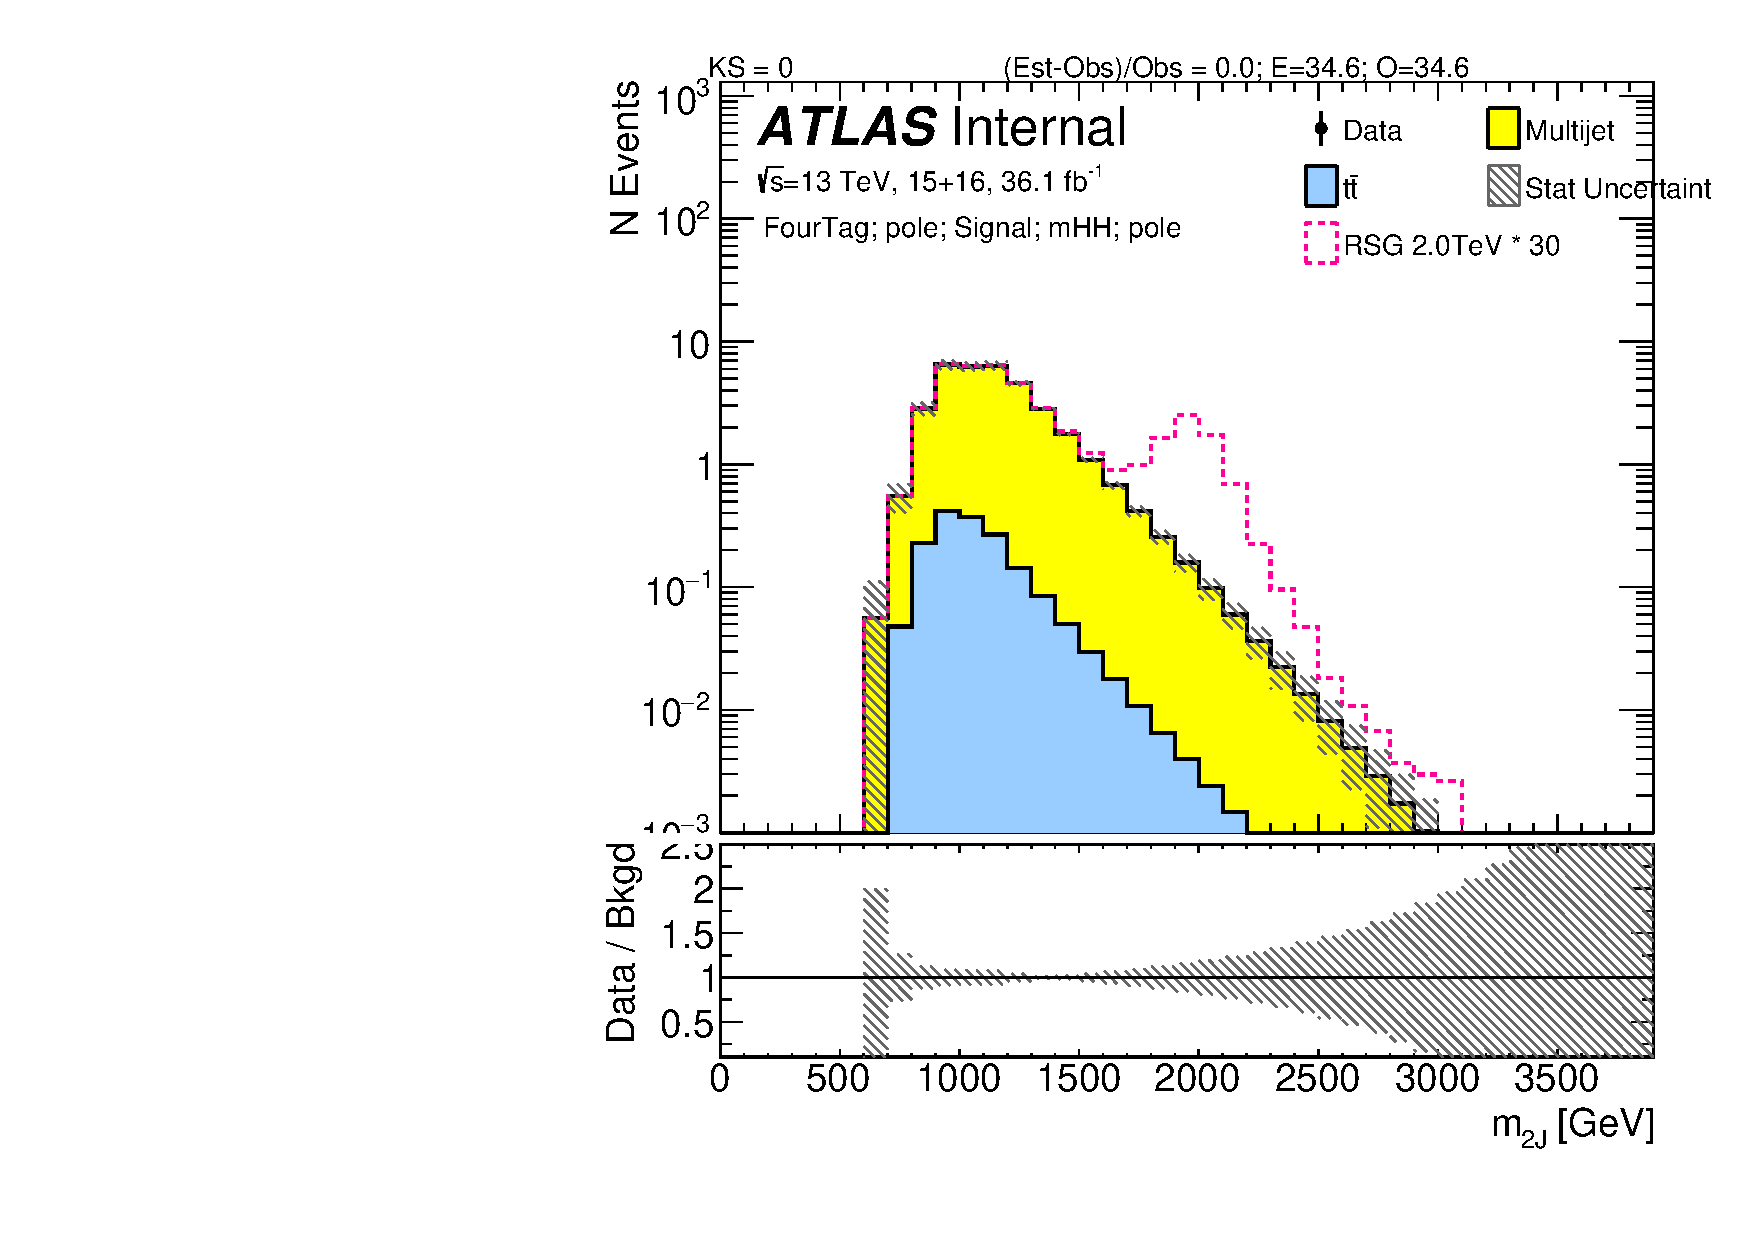
\includegraphics[width=0.45\textwidth,angle=-90]{figures/boosted/Smooth/Moriond_bkg_9_FourTag_pole_Signal_mHH_pole_1_blind.pdf}\\
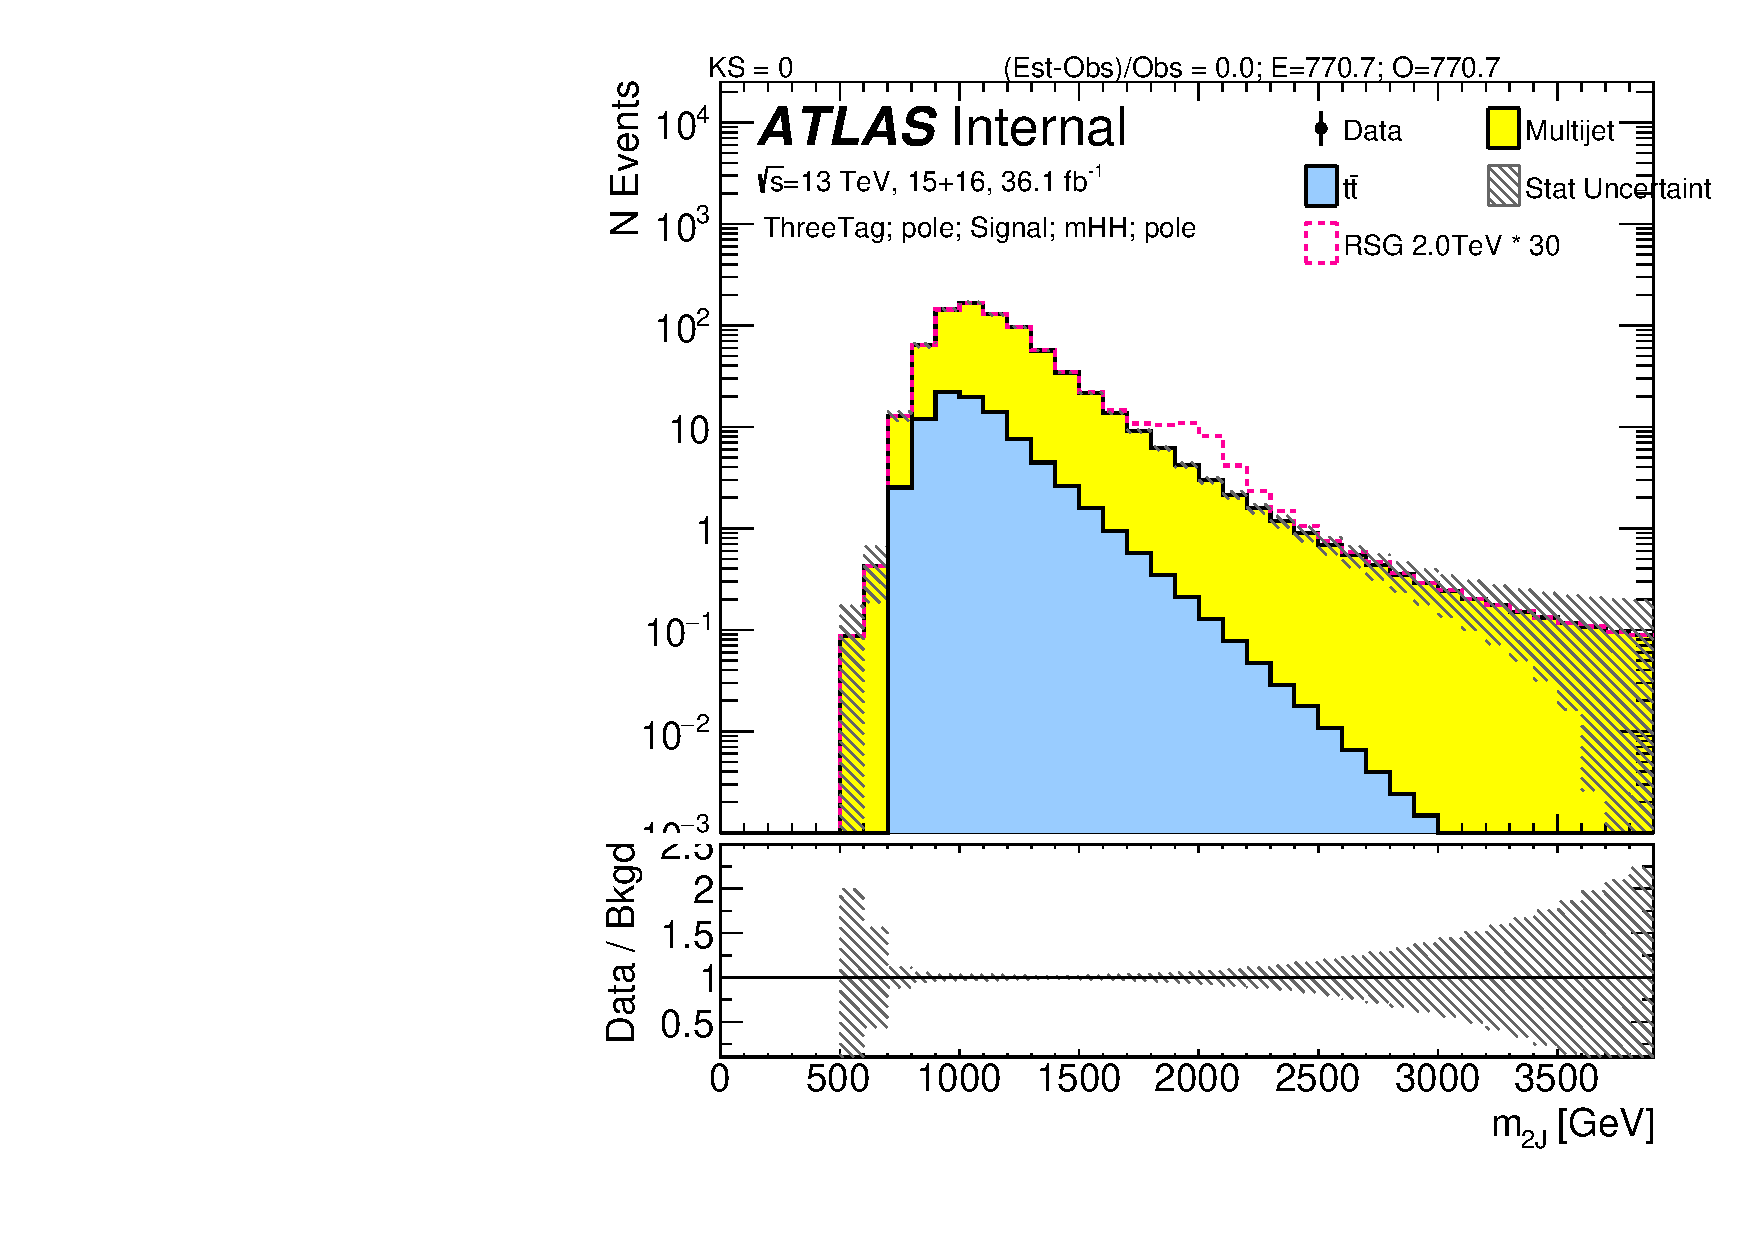
\includegraphics[width=0.45\textwidth,angle=-90]{figures/boosted/Smooth/Moriond_bkg_9_ThreeTag_pole_Signal_mHH_pole_1_blind.pdf}\\
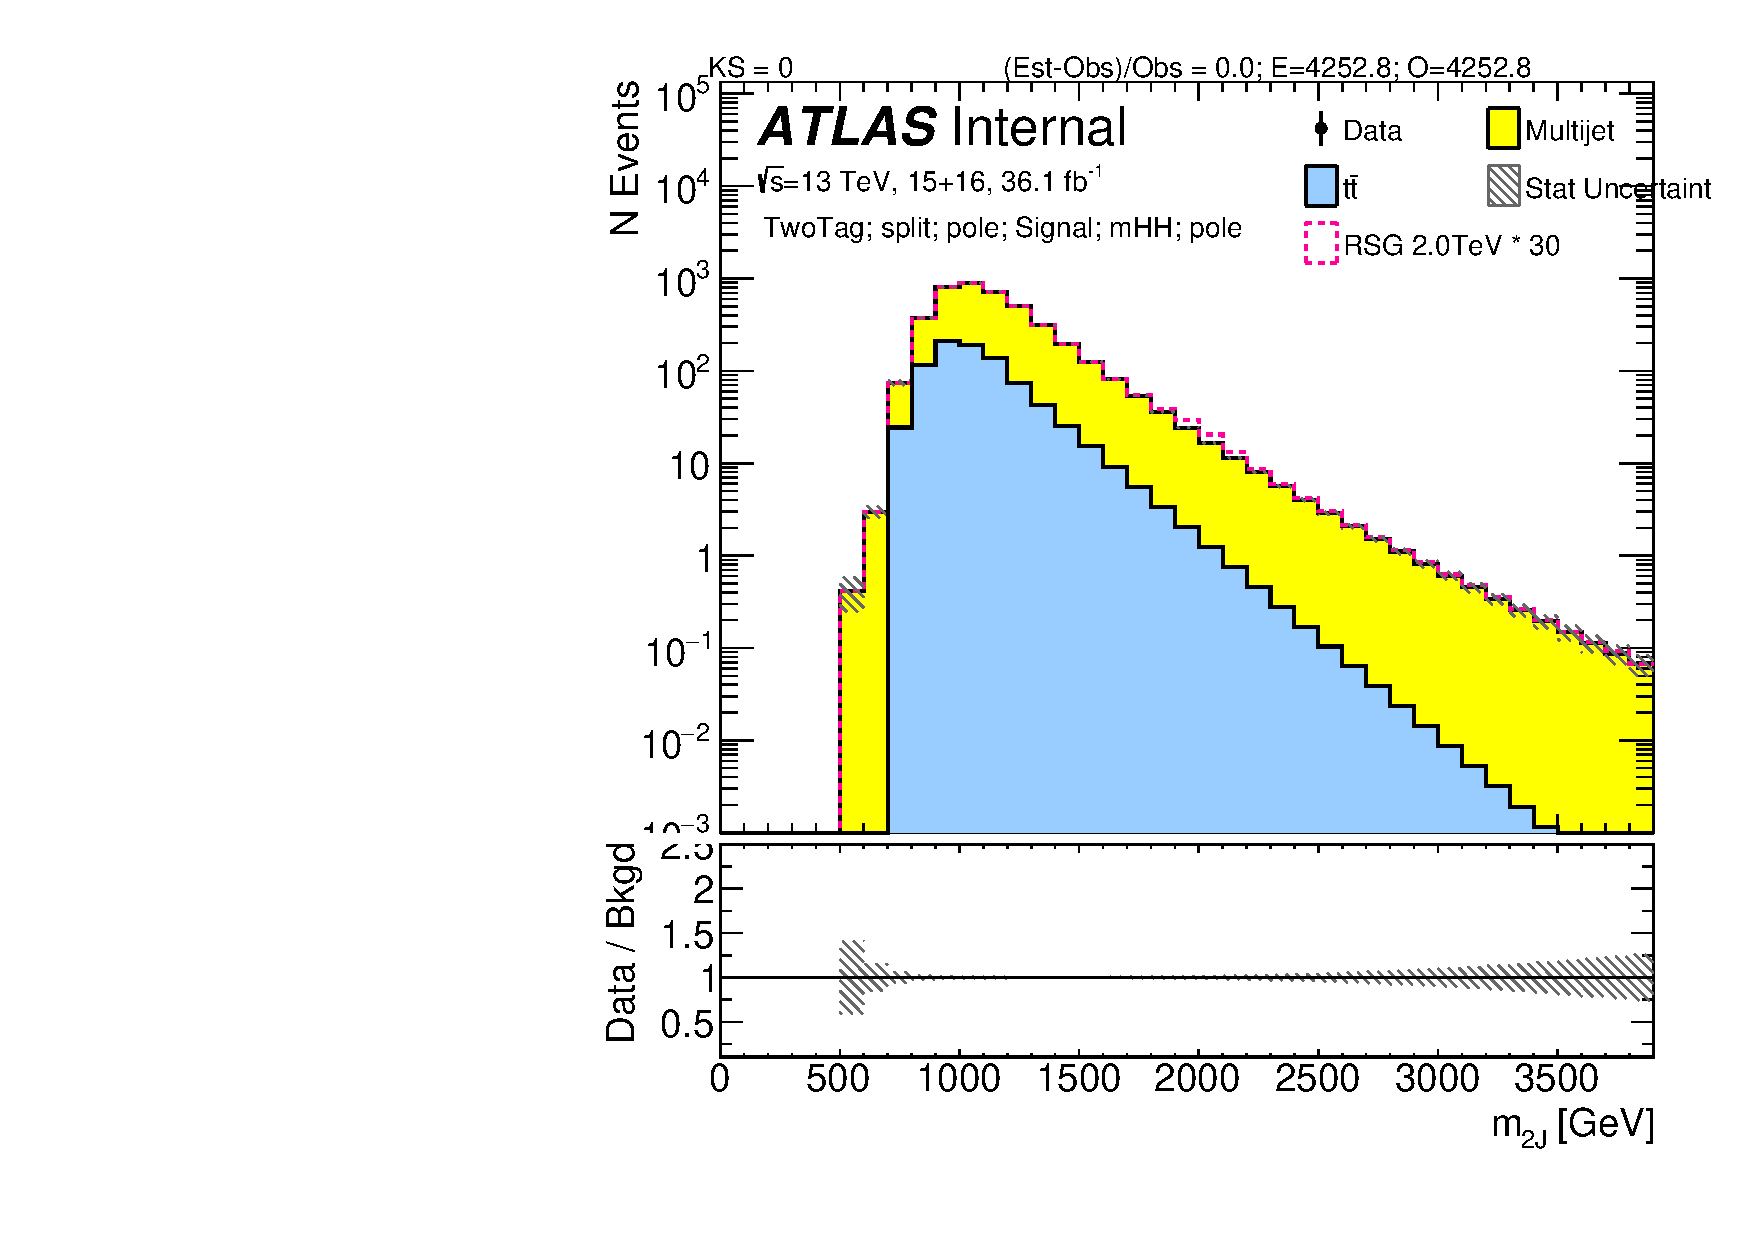
\includegraphics[width=0.45\textwidth,angle=-90]{figures/boosted/Smooth/Moriond_bkg_9_TwoTag_split_pole_Signal_mHH_pole_1_blind.pdf}
\end{center}
\caption{Background prediction for $4b$ (top), $3b$ (middle), and $2bs$ (bottom) signal region using scaled di-jet mass after smoothing. The uncertainty band includes only statistical uncertainties.}
\label{fig:signal-region-mjjscaled-smooth-bkg-noSYS}
\end{figure}
